\pagestyle{empty}
\graphicspath{{Visualizacion/}}
\part{La visualizaci�n}\label{Visualizacion}

\onecolumn

\sffamily

\vspace*{4cm}

En esta parte se describen los conceptos relativos a la visualizaci�n de la informaci�n geogr�fica. Puesto que, a diferencia de lo que sucede en la cartograf�a cl�sica, en un SIG los datos geogr�ficos con los que trabajamos no tienen de por s� una representaci�n fija asociada, est�s ideas son de especial importancia para poder realizar un uso correcto tanto del SIG como de los datos en cuesti�n

\begin{itemize}

\item El cap�tulo \ref{Introduccion_visualizacion} presenta las ideas fundamentales sobre el SIG como herramienta de visualizaci�n. Veremos hasta d�nde alcanzan las capacidades de representaci�n de los SIG y el significado que tienen dentro de este

\item El cap�tulo \ref{Conceptos_basicos_visualizacion} desarrolla las bases te�ricas de la representaci�n visual de la informaci�n, ya sea esta de tipo ge�gr�fico o no. En este cap�tulo no se hace apenas referencia alguna al campo de los SIG, trat�ndose de ideas generales aplicables en cualquier �mbito.

\item En el cap�tulo \ref{El_Mapa} veremos m�s acerca de los mapas, que constituyen los elementos b�sicos de visualizaci�n de la informaci�n geogr�fica. Nos centraremos especialmente en los tipos de mapas existentes y en las peculiaridades y utilidad de cada uno de ellos.

\item El cap�tulo \ref{Visualizacion_SIG} particulariza todo lo anterior para el caso de trabajar con un SIG. De car�cter eminentemente pr�ctico, desarrolla los elementos que encontramos	 en un SIG para crear representaciones visuales y, bas�ndose en lo visto en los otros cap�tulos de esta parte, profundiza en la mejor forma de hacerlo para los distintos tipos de datos geogr�ficos que podemos encontrar en un SIG.

\end{itemize}

\rmfamily
%\twocolumn
\chapter{Introducci�n. Los SIG como herramientas de visualizaci�n}\label{Introduccion_visualizacion}
\pagestyle{fancy}

\begin{keypoints}
�Qu� papel juega la visualizaci�n en un SIG? $\bullet$ �Qu� posibilidades encontramos en un SIG para crear representaciones gr�ficas con la informaci�n geogr�fica? $\bullet$ �Qu� otras aplicaciones pueden efectuar un trabajo similar a un SIG en lo que a la visualizaci�n respecta? $\bullet$ �Qu� relaci�n existe entre los SIG y estas aplicaciones?
\end{keypoints}

\bigskip

\begin{intro}
La representaci�n de la informaci�n geogr�fica es una parte fundamental en el trabajo con SIG, y habitualmente durante una sesi�n de trabajo aparece la necesidad de crear alg�n tipo de representaci�n visual. Antes de entrar en los siguiente cap�tulos de esta parte y detallar los conceptos de representaci�n que despu�s emplearemos para visualizar la informaci�n geogr�fica, veremos en este lo que esta representaci�n implica dentro de un SIG. Estudiaremos los SIG como herramientas que permiten visualizar la informaci�n geogr�fica, analizando sus puntos d�biles y sus aspectos m�s destacados, y veremos c�mo est�n concebidos de cara a satisfacer las diversas necesidades que aparecen en este terreno.

Puesto que vamos a tratar las capacidades de los SIG para la visualizaci�n, con especial atenci�n a las de los SIG de escritorio, los conceptos del cap�tulo \ref{SIGs_escritorio} dedicado a �stos deben conocerse con detalle. Tambi�n es interesante recordar las ideas sobre \emph{Web mapping} descritas en el cap�tulo \ref{Servidores_y_clientes_remotos}.\index{Web mapping}
\end{intro}


\section{Introducci�n}

Visualizar la informaci�n geogr�fica es una parte fundamental del trabajo con un SIG. Aunque no es un aspecto imprescindible, y es posible incluso encontrar SIG enfocados al an�lisis en los cuales no existe forma de visualizar la informaci�n con la que se trabaja, la gran mayor�a de soluciones, especialmente las de escritorio, incluyen las funcionalidades de visualizaci�n como elemento b�sico, y estas resultan imprescindibles para la inmensa mayor�a de usuarios.

Como ya vimos en el cap�tulo dedicado a las herramientas de escritorio, dos son las tareas que un SIG debe permitir en lo que a visualizaci�n respecta: crear representaciones dentro del entorno mismo del SIG y generar representaciones autocontenidas que puedan imprimirse y den lugar a un documento cartogr�fico en sentido cl�sico. La representaci�n en pantalla dentro del SIG puede guardar similitud con la idea cl�sica de mapa, o bien ser distinta, aprovechando elementos que no son habituales en esos mapas y que la tecnolog�a del SIG s� que permite.

En ambos casos, no obstante, lo m�s relevante de cara a los conocimientos que el usuario del SIG debe tener en cuanto a visualizaci�n es la capacidad de convertir los datos en elementos visuales, con independencia de que estos vayan a representarse y usarse en pantalla durante una sesi�n de trabajo, o bien vayan a imprimirse en papel para su uso posterior en ese soporte. Este es el objetivo de esta parte del libro: proporcionar las ideas fundamentales para que el usuario de SIG logre las mejores representaciones visuales durante su trabajo con el SIG. Para ello, lo primero es conocer qu� nos ofrece un SIG como herramienta de visualizaci�n y qu� podemos esperar de �l.


\section{Particularidades del SIG como herramienta de visualizaci�n}

Como herramienta de visualizaci�n, el SIG tiene sus particularidades, las cuales deben unirse a las propias de los modelos de almacenamiento que empleamos para recoger la informaci�n geogr�fica a visualizar. Esto hace que el trabajo de generar una representaci�n visual de una determinada informaci�n geogr�fica no sea igual en el caso de realizarse mediante un SIG que cuando se lleva a cabo en base a la labor cl�sica del cart�grafo. Trabajar en un SIG a�ade, entre otros elementos, el hecho de que la informaci�n se encuentra almacenada seg�n un modelo dado (r�ster o vectorial). Si esta distinci�n implica, como ya sabemos, notables diferencias a la hora de analizar esa informaci�n u optimizar el acceso a los datos que la contienen, no es menos cierto que tambi�n va a conllevar un enfoque distinto a la hora de visualizar unos u otros tipo de datos.

Para el cart�grafo en su concepto cl�sico, esta distinci�n no existe. Indirectamente, s� puede asumirse que existe algo similar, ya que el cart�grafo ha de conocer la naturaleza de las variables que representa, y sabemos que esta naturaleza se encuentra muy ligada al modelo a escoger para representarla (por ejemplo, sabemos que variables continuas como la elevaci�n se analizan mejor si se almacenan seg�n el modelo r�ster, aunque ello no implica que no puedan almacenarse de un modo distinto y ello no tenga inter�s). No obstante, no existe una divisi�n formal explicita tal como sucede en el caso del SIG.

Otra de las diferencias a la hora de representar la informaci�n geogr�fica en un SIG deriva del propio objetivo que dicha representaci�n tiene. La labor del cart�grafo tiene como fin primordial el crear un elemento visual que transmita la informaci�n geogr�fica. El cart�grafo, por lo general, no es un usuario de la cartograf�a, sino un productor de esta para su uso por terceros. El usuario de SIG, sin embargo, puede crear cartograf�a para otros pero, en la mayor�a de los casos, la crea para s� mismo para poder emplearla como una herramienta m�s a la hora de desarrollar su trabajo con el SIG. Por esta raz�n, la representaci�n visual que se produce con un SIG puede tener un car�cter general y estar pensada para ser empleada en �mbitos diversos, pero tambi�n puede tener una funcionalidad muy clara dentro de un campo de aplicaci�n dado, o incluso dentro exclusivamente de un proyecto concreto. Este hecho puede relajar las exigencias que se presentan al generar una representaci�n cartogr�fica en un SIG, pero al mismo tiempo tambi�n ofrece la posibilidad de enfocar el esfuerzo de visualizaci�n de forma m�s particular. Es decir, de considerar el contexto de ese �mbito de utilizaci�n para lograr una representaci�n m�s eficaz dentro de ese entorno particular.

Por �ltimo, cuando pensamos en un mapa tradicional es dif�cil advertir que se trata de un elemento visual creado a partir de otro no visual. Es decir, un mapa es un elemento gr�fico desarrollado a partir de unos ciertos datos. Los datos en s� no pueden <<verse>>, pero son los que posibilitan la creaci�n del mapa. Resulta m�s sencillo pensar que el cart�grafo simplemente plasma la realidad del terreno (que podemos ver con nuestros propios ojos sin m�s que ir a la zona representada por el mapa), que pensar que est� convirtiendo datos en elementos gr�ficos tales como l�neas o puntos. Sin embargo, y aunque no utilicemos un SIG, esos datos existen, ya que el cart�grafo pone sobre el papel las medidas (datos num�ricos) tomados por los t�cnicos en campo, ya sean estas provenientes de alg�n sensor o el resultado de un levantamiento topogr�fico, entre otros or�genes posibles. 

El beneficiario de esos datos es el usuario del mapa, que recibe la representaci�n visual de �stos, y es esta visualizaci�n la que le transmite, en la medida de lo posible y en funci�n de su propia calidad como elemento de comunicaci�n, la informaci�n geogr�fica subyacente. El usuario de un SIG, salvo que utilice una imagen (una fotograf�a a�rea, un mapa escaneado o un mapa ya preparado a trav�s de un servicio de mapas), no recibe elemento visual alguno, sino tan solo datos num�ricos que son, eso s�, muy susceptibles de ser visualizados.\index{Escaneo}

En relaci�n con esto, un SIG est� pensado para satisfacer dos necesidades fundamentales. Por una parte, la creaci�n de cartograf�a a partir de los datos, del mismo modo que el cart�grafo utiliza otro tipo de herramientas para elaborar mapas a partir de los datos topogr�ficos o tem�ticos de los que dispone. Por otra, y para el usuario cuyo fin �ltimo no es la elaboraci�n de cartograf�a, visualizar de la mejor forma posible los datos con los que trabaja, para que esta visualizaci�n aporte valor a�adido a los datos de cara al desarrollo de la labor de ese usuario. Ambos enfoques coexisten en un SIG y est�n orientados en cualquier caso a extraer de los datos la mayor informaci�n posible de forma visual.

En definitiva, debemos tener siempre presente que en un SIG la informaci�n geogr�fica no es un elemento visual, ya que llega a nosotros convertida en �ltima instancia en algo puramente num�rico, apto para ser procesado de un modo u otro por el ordenador en el que ejecutamos el SIG. Somos nosotros, a trav�s del SIG, quienes la dotamos de un aspecto visual. En otras palabras, en un mapa cl�sico la tarea del cart�grafo (que es quien prepara la informaci�n geogr�fica) es hacer que sea lo m�s f�cil posible de interpretar para el usuario de ese mapa. En el SIG existe tambi�n alguien que prepara los datos (por ejemplo, un t�cnico que comprueba la calidad de un MDE y lo almacena en un formato dado), pero su objetivo es facilitar su interpretaci�n y uso al ordenador (o, m�s concretamente, al SIG). La visualizaci�n, por lo general, y salvo que en esa preparaci�n se a�adan elementos adicionales que complementen al dato en s�, queda en manos del usuario del dato. Es por esta raz�n que una parte como esta resulta fundamental en un libro de SIG, ya que el usuario de SIG necesita conocer c�mo emplear el SIG para visualizar la informaci�n con la que trabaja.

\section{La visualizaci�n cient�fica y los SIG}

Aunque, como decimos, el SIG hace m�s obvio que un mapa es la expresi�n visual de una serie de datos, la visualizaci�n de datos no es algo exclusivo de los SIG como aplicaciones inform�ticas, y en absoluto se trata de algo nuevo relacionado con los ordenadores y sus capacidades de representaci�n. La creaci�n de gr�ficas y diagramas es una realidad desde mucho antes que aparecieran los ordenadores, y estas son una herramienta fundamental en el �mbito cient�fico. Visualizar series de datos sencillos mediante la representaci�n de �stos ayuda a comprender su naturaleza y constituye un �til de gran potencia a pesar de su aparente simplicidad.

Visualizando un dato cualquiera se obtiene una densidad de informaci�n mucho mayor que si ese mismo dato se representa num�rica o textualmente. Asimismo, se estima que aproximadamente el 50\% de las neuronas est�n dedicadas a la visualizaci�n. Como reza la sabiduria popular, <<una imagen vale m�s que mil palabras>>, y esta es una verdad que cobra pleno sentido dentro de campo de las ciencias.


Se puede pensar que una representaci�n simple tal como un diagrama de barras o uno de dispersi�n est� muy alejado del tipo de representaci�n compleja que un mapa supone, y que, por tanto, tambi�n es muy distinta de la representaci�n que tiene lugar en un SIG. Analiz�ndolo con un poco m�s de detalle vemos, sin embargo, que la diferencia no es tal y existen muchas similitudes y relaciones.

En primer lugar, estas representaciones pueden aplicarse a la componente tem�tica de los datos espaciales y permitir el an�lisis de esta. Prescindiendo de la componente espacial, la componente tem�tica es susceptible de ser analizada mediante cualquiera de las herramientas habituales de la estad�stica descriptiva, entre ellas las del an�lisis exploratorio de datos tales como las gr�ficas y diagramas antes mencionados.

En segundo lugar, existen en la actualidad otras herramientas de visualizaci�n de datos m�s avanzadas, producto del avance tecnol�gico de los �ltimos tiempos, el mismo que ha propiciado el salto de la cartograf�a cl�sica a la cartograf�a digital y al campo de los SIG. Si el volumen de informaci�n y sus caracter�sticas ha variado sensiblemente en lo que al �mbito geogr�fico respecta, otras �reas no han sido ajenas a transformaciones similares, lo cual ha tenido como consecuencia el desarrollo de nuevas ideas para poder visualizar esa informaci�n y poder aprovechar sobre ella las capacidades de percepci�n y an�lisis visual de que disponemos. El desarrollo en este sentido es tal que constituye en la actualidad una rama de la ciencia propia: la \emph{visualizaci�n cient�fica}.\index{Visualizaci�n cient�fica}

Los conceptos de la visualizaci�n cient�fica pueden ser aprovechados por los SIG, que aproximan de ese modo sus funcionalidades a las de las aplicaciones de visualizaci�n gen�rica de datos. En algunos casos, las diferencias son meramente formales y debidas a los enfoques tradicionales que se vienen empleando en estos campos, pero la integraci�n entre ambos es posible al menos en lo que a sus conceptos y fundamentos respecta.

Consideremos por ejemplo, las representaciones de la figura \ref{Fig:VisualizacionCientifica}. La de la izquierda se ha producido a partir de datos obtenidos en un t�nel de viento y muestra las presiones ejercidas por el aire sobre un ciclista, as� como las lineas de flujo que se forman. La de la derecha representa la actividad cerebral en un rat�n tras un est�mulo, y se ha creado en base a los datos proporcionados por un tom�grafo. Salvando las diferencias en cuanto al campo de la ciencia del que provienen, ambas representaciones guardan muchas semejanzas con, por ejemplo, las obtenidas a partir de un MDE, en las que habitualmente se emplea una paleta de colores similar para visualizar los valores de las distintas celdas. Puedes ir al cap�tulo \ref{Creacion_capas_raster} para encontrar un buen n�mero de ellas y comprobar por ti mismo esa similitud.	\index{Tom�grafo}

\begin{figure}
\centering
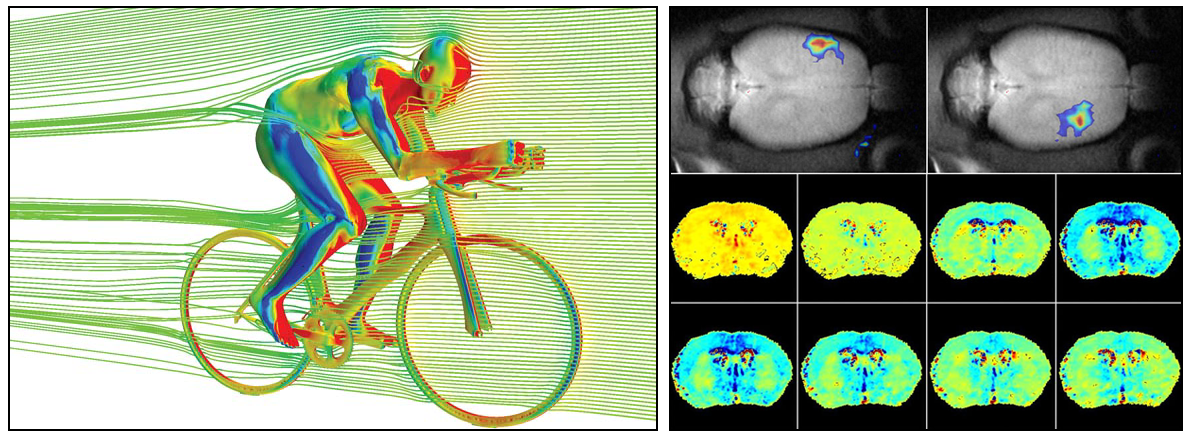
\includegraphics[width=\mycolumnwidth]{Introduccion_visualizacion/SciVis.png}
\caption{\small Dos ejemplos de visualizaci�n cient�fica.}
\label{Fig:VisualizacionCientifica} 
\end{figure}


Aunque puedan parecer algo muy alejado de lo que entendemos por SIG y del trabajo que desarrollamos con uno de ellos, lo cierto es que representaciones as� podr�an perfectamente formar parte de un proyecto SIG, al menos en teor�a. Si pensamos en la primera de ellas, la del ciclista, no es raro en la actualidad que un SIG 3D permita cargar modelos tridimensionales tales como edificios o �rboles, por poner dos ejemplos (veremos esto con detalle algo m�s adelante en esta misma parte del libro). De este modo, no es tan descabellado pensar en disponer en un SIG de los datos de la forma de ese ciclista, datos que, por otra parte, son de tipo espacial y encajan perfectamente en el tipo de datos que un SIG maneja. De hecho, el modelo que ha servido para calcular esos datos de presi�n podr�a aplicarse mediante las capacidades de modelizaci�n de un SIG, y podr�a estudiarse un supuesto en el que se conocieran los datos de viento de una determinada zona. Es decir, situar al ciclista en una calle dada y con unas condiciones concretas y efectuar el c�lculo que nos llevar�a a unos datos similares a los representados en la imagen. Siendo posible realizar ese c�lculo en un SIG, visualizar esos datos resultantes a trav�s de una representaci�n como la mostrada es, sin embargo, algo que no resulta a�n posible en un SIG, y es necesario el concurso de una aplicaci�n especializada de visualizaci�n cient�fica.

As� pues, las im�genes de la figura \ref{Fig:VisualizacionCientifica} no han sido creadas con un SIG, sino con sendas aplicaciones de visualizaci�n cient�fica de ese tipo. Estas aplicaciones presentan funcionalidades distintas a las que tiene un SIG, siendo habitualmente m�s avanzadas y con un mayor grado de interactividad. Asimismo, est�n pensadas para la representaci�n de datos multidimensionales, algo que no sucede con los SIG \cite{McCormick1987ACM}. La diferencia principal estriba en que, mientras que la visualizaci�n en el SIG complementa al an�lisis y a otras operaciones sobre los datos, en la visualizaci�n cient�fica esta \emph{es} el an�lisis, y el objetivo �nico de la visualizaci�n es facilitar el an�lisis visual de los datos. Este es el motivo por el que aparecen funciones avanzadas de tipo interactivo que permiten al usuario <<jugar>> con los datos, alterando su representaci�n para hacer m�s explicita la informaci�n que contienen.

Si estas funcionalidades avanzadas no aparecen en los SIG en la actualidad, esto no obedece a una imposibilidad t�cnica o a que carezca de sentido implementarlas, sino m�s bien al enfoque predominante en el dise�o de los SIG, que en lo que a visualizaci�n respecta se asemeja mucho a�n a la cartograf�a cl�sica. Aunque los SIG 3D van ganando terreno, la idea cl�sica de visualizaci�n en un SIG hereda directamente del mapa tradicional, y se constituye en muchos casos como una mera herramienta para crear este, sin considerar que puede ser posible la creaci�n de otro tipo de representaciones.

Las limitaciones en cuanto a visualizaci�n tambi�n se deben en parte a las limitaciones en los datos, ya que un SIG no es de momento la herramienta ideal para el manejo de datos multidimensionales, a pesar de que estos abundan en el �mbito geogr�fico. Hemos estudiado mucho acerca de los datos espaciales en este libro, y la mayor parte de cuanto hemos visto se basa en el uso de geometr�as planas o, en todo caso, tridimensionales, siendo extra�o el trabajo con otros datos, al menos en los SIG de uso gen�rico. Existen, por ejemplo, modelos para mallas de datos multidimensionales, pero las capas r�ster tal y como las hemos estudiado son puramente bidimensionales. Mientras haya carencias en los modelos de datos y en la concepci�n del dato geogr�fico, es l�gico entender que las capacidades de visualizaci�n de los SIG tambi�n presenten deficiencias a la hora de trabajar ciertos tipos de datos

El uso combinado de aplicaciones para visualizaci�n cient�fica y SIG es la soluci�n actual a determinados problemas de visualizaci�n que exceden las capacidades habituales de estos �ltimos. En este sentido, se han producido acercamientos entre ambos tipos de aplicaciones para tratar de conseguir que esta combinaci�n no se lleve a cabo tan solo mediante una mera compartici�n de datos (uso de formatos comunes que permiten <<pasar>> los datos de una aplicaci�n a otra), sino que exista una verdadera integraci�n que reduzca la redundancia de funcionalidades y maximice las posibilidades. Por el momento, la plena integraci�n dista mucho de ser una realidad, por lo que debe recurrirse a la utilizaci�n conjunta de una u otra manera. En \cite{Rhyne1997CG} puede encontrarse este tema desarrollado con m�s profundidad.

Aunque en los SIG faltan muchos de los elementos y de las capacidades de las aplicaciones de visualizaci�n cient�fica, algunas ideas de esta s� que aparecen en ellos, y en su conjunto ampl�an la potencialidad del mapa como met�fora de una realidad que se representa. La m�s b�sica de todas ellas es la interactividad que permiten las herramientas de navegaci�n. Aunque lejanas de lo que podemos encontrar en aplicaciones de visualizaci�n cient�fica especializadas, ofrecen un respuesta por parte del mapa a las acciones de quien lo utiliza. Frente al car�cter pasivo del mapa impreso, las representaciones dentro de un SIG son activas. 

Otros elementos menos frecuentes son la incorporaci�n de animaciones y la visualizaci�n tridimensional. Sin ser equiparable a las capacidades de representaci�n multidimensional de un programa de visualizaci�n cient�fica, esta �ltima supone, no obstante, un salto cualitativo enorme frente al car�cter bidimensional del mapa impreso. En el cap�tulo \ref{Visualizacion_SIG} veremos m�s acerca de las representaciones tridimensionales y las animaciones.

Este nuevo enfoque que se produce en el �mbito cartogr�fico al incorporar parte de las ideas de la visualizaci�n cient�fica se conoce como \emph{geovisualizaci�n}, y conforma una rama de esta �ltima dedicada al caso particular de visualizar la informaci�n geogr�fica. Una forma muy gr�fica de ver la diferencia entre el documento cartogr�fico cl�sico y la geovisualizaci�n que se produce dentro de un SIG es mediante el denominado \emph{Cubo cartogr�fico} \cite{MacEachren1994Pergamon} (Figura \ref{Fig:CuboCartografico}).\index{Cubo cartogr�fico}\index{Geovisualizaci�n}

\begin{figure}
\centering
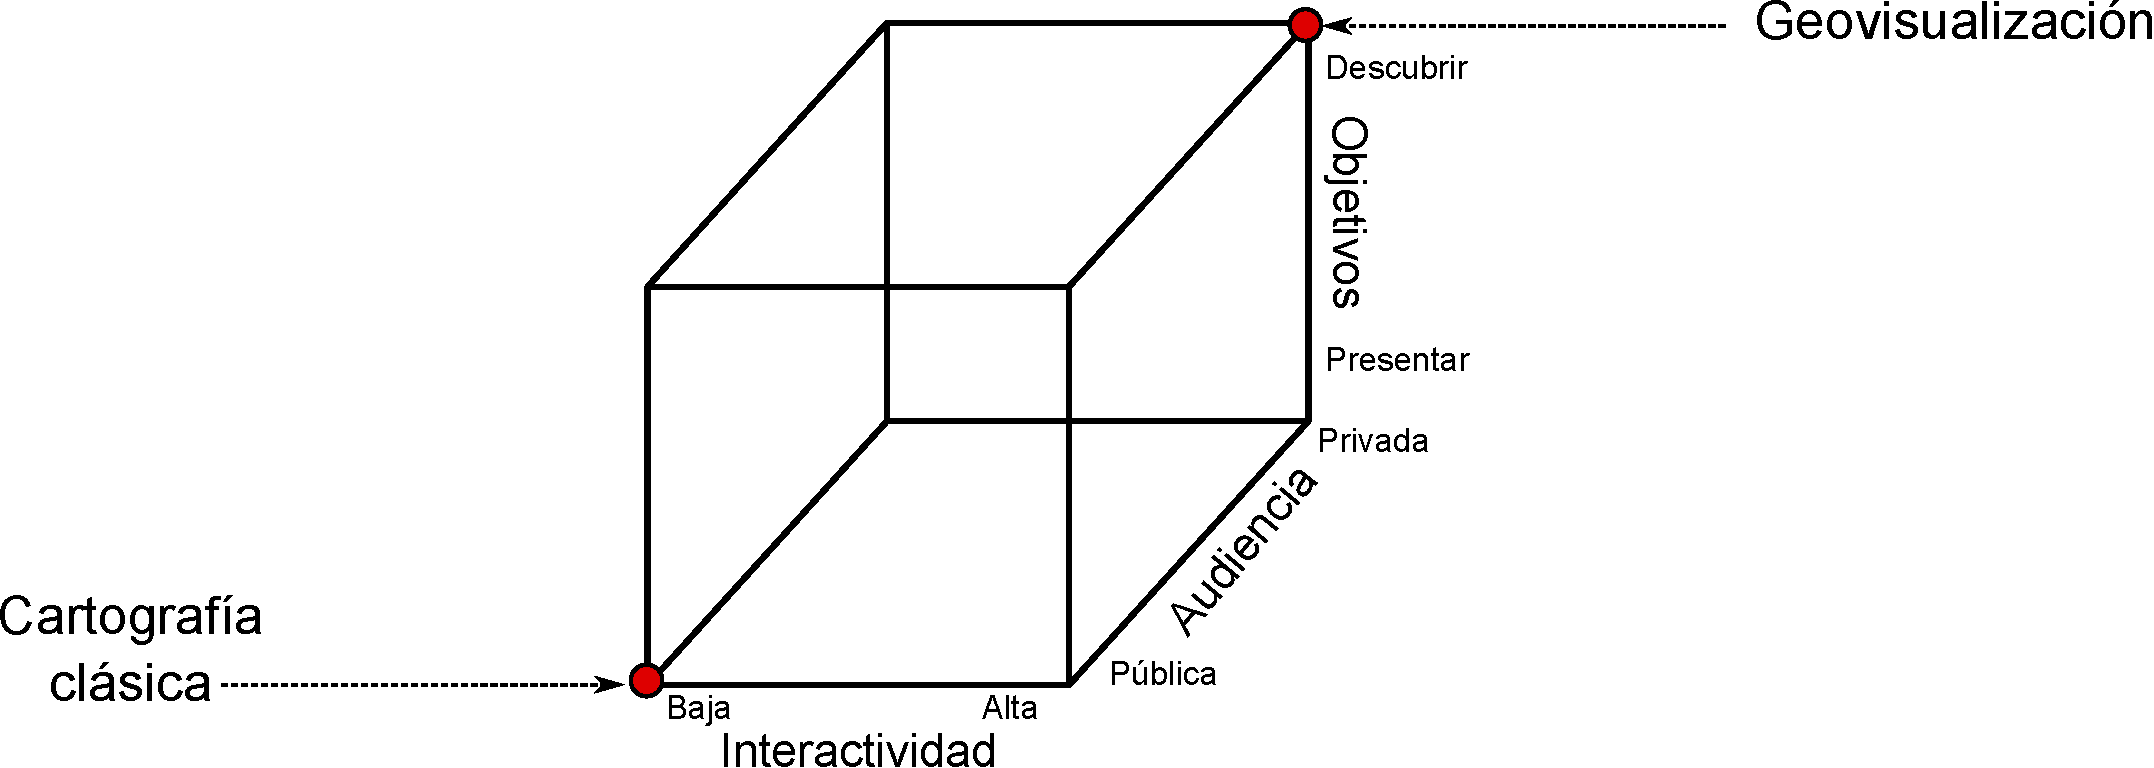
\includegraphics[width=0.85\mycolumnwidth]{Introduccion_visualizacion/CuboCartografico.pdf}
\caption{\small El \emph{cubo cartogr�fico}.}
\label{Fig:CuboCartografico} 
\end{figure}

El cubo cartogr�fico contiene tres ejes, en los cuales se representan el grado de interactividad, el objetivo principal de la representaci�n y la audiencia a la que esta se dirige. La cartograf�a cl�sica y la geovisualizaci�n se sit�an en v�rtices opuestos, ya que presentan caracter�sticas distintas en estos tres conceptos. El mapa cl�sico esta pensado para presentar una informaci�n de la que ya se dispone, pero no es una herramienta para descubrir nueva informaci�n. La geovisualizaci�n, por el contrario, con la posibilidad que ofrece al usuario de <<explorar>> los datos, puede servir para extraer informaci�n que no se conoc�a de antemano a la hora de crear la representaci�n. La interactividad es alta en la geovisualizaci�n y baja en el mapa cl�sico, como ya hemos visto. Por �ltimo, la audiencia en la geovisualizaci�n es privada, entendi�ndose con esto no que existan restricciones para su acceso, sino que en su mayor�a son representaciones fugaces que cambian seg�n el usuario interact�a con el \emph{software}, y por tanto lo normal es que solo sea ese usuario quien las disfrute, no teniendo un car�cter persistente como el mapa impreso.


\section{Los SIG frente a las aplicaciones de dise�o}

Pese a que, como acabamos de ver, la visualizaci�n en un SIG va mucho m�s all� del mapa tradicional, resulta indudable que la creaci�n de este es una tarea fundamental y que los SIG han de responder a esa necesidad como herramientas primordiales para el cart�grafo y el dise�ador. No obstante, como ya se mencion� en \ref{GeneracionCartografia}, las necesidades del cart�grafo van a menudo m�s all� de los que un SIG puede ofrecer, siendo necesario recurrir a programas de dise�o del mismo modo que sucede con las aplicaciones de visualizaci�n cient�fica. Esto es as�, principalmente, debido a que la labor del cart�grafo contiene un elemento art�stico (que es, a su vez, puramente visual) que los SIG no est�n preparados para manejar. El SIG es una herramienta demasiado <<estricta>> en este sentido, ya que realiza una representaci�n de los datos donde prima la exactitud y la correcci�n, sin dejar lugar para licencias que, si bien mejorar�n la calidad del mapa como medio de transmisi�n de informaci�n, suponen un elemento fuera de la ortodoxia del SIG.

As�, un cart�grafo puede necesitar representar un punto o una l�nea desplazada de su localizaci�n real o deformar alg�n elemento, y esto es algo que, en general, un SIG no permite. En realidad, no es algo imposible de hacer en un SIG, sino, por el contrario, algo sencillo. Bastar�a modificar los datos para adaptarlos a la visualizaci�n que queremos obtener. De este modo, no obstante, estamos alterando el dato y creando uno nuevo incorrecto, lo cual afectar� a cualquier otro uso posterior que se haga de est� m�s all� de su visualizaci�n. Es decir, el SIG no permite mantener la correcci�n de los datos y al mismo a�adir esas <<incorrecciones>> que forman parte de las herramientas del cart�grafo a la hora de crear cartograf�a.

La soluci�n es, como hemos dicho, hacer uso de aplicaciones de dise�o que no tienen en consideraci�n el significado de los elementos gr�ficos y no plantean restricciones como las anteriores. Esto puede llevarse a cabo operando con el SIG para crear una primera representaci�n que luego se edita en un programa de dise�o gr�fico para retocar aquellos elementos que puedan mejorarse mediante el buen hacer del cart�grafo experimentado. En particular, el uso de \emph{software} de ilustraci�n vectorial es la opci�n m�s adecuada para la elaboraci�n de mapas. Este planteamiento supone, sin embargo, una integraci�n muy d�bil y que presenta numerosos inconvenientes, entre los cuales cabe citar los siguientes:

\begin{itemize}
	\item Incapacidad de la aplicaci�n de dise�o para analizar los datos. La representaci�n puede hacerse de forma completamente manual, creando cada uno de sus elementos y definiendo sus caracter�sticas sin la ayuda de ninguna rutina, pero tambi�n puede llevarse a cabo haciendo uso de alguna funcionalidad suplementaria. Por ejemplo, para establecer los colores de los distintos pol�gonos de una capa puede usarse el valor de uno sus atributos y establecer una rampa de colores en funci�n de este. El SIG puede hacer esto autom�ticamente, pero una aplicaci�n de dise�o, puesto que no puede interpretar esos atributos y carece de esa funcionalidad, requerir� que el cart�grafo lleve a cabo esa asignaci�n de colores de modo manual.
	\item Dificultad de actualizaci�n. Al no estar la representaci�n sincronizada con la base de datos, las modificaciones en esta no le afectan, y es necesario rehacer los mapas cada vez que los datos cambien, ya que esa actualizaci�n no se produce de forma autom�tica.
	\item Nula o muy limitada capacidad de automatizaci�n de tareas. Un SIG puede automatizar tareas tales como la subdivisi�n de un mapa en submapas menores (v�ase la imagen \ref{Fig:Serie_mapas}) o la producci�n de mapas sobre un conjunto de capas. Por ejemplo, podemos <<mostrarle>> al SIG c�mo queremos el dise�o del mapa de una variable dada y que �l se encargue de generar los mapas de ese modo para otra serie de variables recogidas en otras tantas capas en nuestra base de datos. Puesto que la aplicaci�n de dise�o gr�fico no puede por s� misma acceder a esa base de datos, esta automatizaci�n no es posible en caso de crear cartograf�a con ella.  
	\item Mayor posibilidad de introducir errores cartogr�ficos. La permisividad de una aplicaci�n de dise�o gr�fico es un arma de doble filo. Por una lado, permite al cart�grafo tomarse ciertas licencias cuando ello resulta necesario, pero tambi�n cuando no es correcto hacerlo. La aplicaci�n no entiende, por ejemplo, que la orientaci�n del mapa no debe variar si no lo hace tambi�n la rosa de los vientos o que el \emph{canev�s} (la rejilla que acompa�a al mapa) debe estar correctamente situado, y permite que se introduzcan errores que en un SIG se encuentran completamente controlados.\index{Canev�s}
\end{itemize}
	
	
Al contrario de lo que suced�a con las herramientas de visualizaci�n cient�fica, los SIG s� que van progresivamente incorporando la ideas de estas aplicaciones de dise�o gr�fico, permitiendo cada vez m�s la labor art�stica del cart�grafo y adapt�ndose a sus necesidades igual que se adaptan a las de otros usuarios con requerimientos distintos de visualizaci�n. A�n as�, este tipo de capacidades deben considerarse como algo avanzado que pocos SIG incorporan, ya que la mayor�a de ellos se centran en la visualizaci�n dentro de su propio entorno y solo permiten la elaboraci�n de cartograf�a rudimentaria o, al menos, lejos de los est�ndares de la producci�n cartogr�fica cl�sica.


\section{Resumen}

La visualizaci�n es parte vital de los SIG y por ello estos disponen de abundantes funcionalidades para la representar la informaci�n geogr�fica. Existen, no obstante, importantes diferencias entre la creaci�n de una representaci�n dentro de un SIG y la labor tradicional del cart�grafo. Desde el punto de vista conceptual, una diferencia fundamental es el hecho de que el usuario de la informaci�n geogr�fica en un SIG no la recibe en un formato visual, sino como meros datos num�ricos, siendo �l quien ha de procurarse esa representaci�n visual.

La visualizaci�n de datos es en la actualidad un apartado de gran importancia no solo en el campo del SIG, sino en todo el �mbito cient�fico en general. Las aplicaciones existentes para la visualizaci�n de datos de diversa �ndole superan en muchas ocasiones a los SIG en cuanto a sus capacidades, especialmente en el manejo de datos multidimensionales y la interactividad entre el usuario y la representaci�n. El uso conjunto de estas aplicaciones y los SIG amplia las posibilidades de estos, que por el momento no incluyen dichas capacidades avanzadas entre sus funcionalidades.

Otras aplicaciones que complementan a los SIG en lo que a la producci�n de cartograf�a respecta son las empleadas en el dise�o gr�fico. Las funcionalidades de estas, no obstante, s� que est�n siendo incorporadas progresivamente por los SIG, de tal modo que �stos cada vez van siendo herramientas m�s completas que ofrecen todo lo necesario para la creaci�n profesional de c	artograf�a.
\chapter{Conceptos b�sicos de visualizaci�n y representaci�n}\label{Conceptos_basicos_visualizacion}

\begin{keypoints}
�Qu� debemos conocer para representar la informaci�n geogr�fica de la mejor manera posible? $\bullet$ �Qu� es el lenguaje visual? $\bullet$ �Qu� son las variables visuales? $\bullet$ �Qu� variables visuales existen? $\bullet$ �C�mo afectan a los distintos elementos gr�ficos con que componemos un mapa? $\bullet$ �Qu� propiedades tienen?
\end{keypoints}

\bigskip

\begin{intro}
Puesto que tratamos la visualizaci�n de la informaci�n geogr�fica, resulta necesario conocer algunas de las ideas fundamentales acerca del lenguaje visual para usar este adecuadamente. Con estas, sabremos c�mo hacer mejores representaciones visuales para transmitir una informaci�n dada, aprovechando las propiedades de los elementos del lenguaje de un modo �ptimo. Los conceptos que se detallan en este cap�tulo pueden aplicarse a cualquier tipo de representaci�n visual, por lo que podremos posteriormente trasladarlos al contexto de la cartograf�a.
\end{intro}

\section{Introducci�n}

Cuando visualizamos cualquier tipo de informaci�n geogr�fica, ya sea a trav�s de un mapa cl�sico o de alg�n elemento gr�fico en la pantalla de un ordenador, estamos utilizando un lenguaje visual para transmitirla. Del mismo modo que al hablar empleamos un lenguaje oral y al escribir un lenguaje escrito, siempre que plasmemos la informaci�n geogr�fica en una serie de elementos visuales estaremos empleando este lenguaje visual.

Existen muchas similitudes entre el lenguaje visual y el lenguaje que utilizamos cada d�a para comunicarnos, comunes todas ellas a cualquier forma de lenguaje. Por una parte, disponemos de una serie de elementos b�sicos que podemos usar, que son como las palabras con las que formamos frases y expresamos ideas. Estas se combinan de acuerdo con unas normas y siguiendo esquemas definidos que conocen tanto el creador del mensaje como el receptor, y sin los cuales no seria posible establecer la comunicaci�n. Por otra, el conocimiento y manejo adecuado de todos estos elementos define nuestra capacidad de emplear el lenguaje y expresar correctamente aquello que queremos transmitir.

Al igual que en el lenguaje hablado, y por su car�cter simb�lico, el lenguaje visual implica la existencia de unas limitaciones. Es decir, no podemos expresar todo aquello que tratamos de representar, y un mapa nunca puede contener y transmitir fielmente toda la realidad de una zona o de un fen�meno espacial dado. Sin embargo, un correcto uso del lenguaje permite comunicar gran cantidad de informaci�n y hacer de este una herramienta de gran utilidad, m�s all� de sus limitaciones, o incluso aprovechando estas para su propio beneficio.

El estudio de los signos de un lenguaje constituye lo que se conoce como \emph{semiolog�a}. En el caso de los elementos del lenguaje visual, encontramos una \emph{semiolog�a gr�fica}, tal y como la defini� el cart�grafo franc�s Jacques Bertin, pionero en este campo \cite{Bertin1987Pompidou}. Esta semiolog�a trata los signos del lenguaje visual y la gram�tica de estos, definiendo una ling��stica visual que nos ayuda a comprender c�mo una representaci�n gr�fica dada cumple su prop�sito de transmitir la informaci�n en base a la cual se crea.\index{Bertin, Jacques}\index{Semiolog�a gr�fica}

Detallando las ideas de Bertin, en este cap�tulo veremos algunos aspectos fundamentales acerca del lenguaje visual que nos permitir�n conocer sus propiedades y la forma en que sus elementos pueden emplearse de forma efectiva para la comunicaci�n. Aplicando estos al caso particular de representar y visualizar informaci�n cartogr�fica, expandiremos este en el pr�ximo cap�tulo para obtener un lenguaje cartogr�fico, fundamental para la creaci�n de mapas.


\section{Las variables visuales}

Cada lenguaje tiene sus propiedades particulares y permite expresar unas u otras ideas de distintas maneras. Por ejemplo, podemos plasmar la m�sica en una partitura, utilizando un lenguaje de signos musicales. Este lenguaje musical\footnote{Enti�ndase que hablamos aqu� de ese lenguaje de signos sobre un papel y no del lenguaje musical relativo a una forma de expresi�n a trav�s del ritmo, el tono, etc.} permite recoger y transmitir una canci�n a trav�s de una partitura, expresando mediante un conjunto de s�mbolos las distintas notas que la componen, su duraci�n o los elementos expresivos que deben incorporarse en la interpretaci�n de esta. Un m�sico que conozca este lenguaje puede interpretar una pieza gracias a que la m�sica le llega a trav�s de esos s�mbolos, siendo la partitura el medio de comunicaci�n entre el interprete y el compositor o quien haya transcrito dicha pieza. 

Aunque dos personas conozcan a la perfecci�n el lenguaje musical, no podr�n, sin embargo, transmitirse mediante sus s�mbolos y sus reglas algo como una formula matem�tica o un poema. El lenguaje matem�tico o el lenguaje oral son los adecuados para transmitir este tipo de mensajes, pero no el lenguaje musical, que tiene limitaciones en ese sentido.

Puesto que nuestro objetivo a lo largo de los cap�tulos de esta parte del libro es ser capaces de crear mapas y otros elementos visuales que transmitan la informaci�n geogr�fica, debemos estudiar qu� clase de informaci�n vamos a transmitir y, sobre todo, qu� nos permite transmitir el lenguaje visual. Del mismo modo que sabemos que los s�mbolos de nuestro lenguaje musical (pentagrama, figuras, etc.) no son capaces de transmitir una formula matem�tica, debemos ver si los elementos del lenguaje visual van a ser capaces de, por ejemplo, transmitir el patr�n de distribuci�n de un fen�meno en el espacio, las diferencias entre dos zonas distintas o la relaci�n entre los valores de una variable en dos puntos. Adem�s, debemos ver c�mo emplearlos para que esa informaci�n se transmita de la mejor manera posible, ya que existen diversas propiedades de los elementos visuales que podemos emplear, siendo m�s adecuadas unas u otras seg�n sea la circunstancia.

Estas propiedades conforman lo que se conoce como \emph{variables visuales}, y se aplican a los elementos b�sicos de la representaci�n, que son aquellos objetos geom�tricos de que se compone esta. Las variables visuales permiten diferenciar unos de otros y asignarles unas ciertas caracter�sticas, susceptibles a su vez de ser interpretadas junto al propio significado que el objeto pueda tener. Dados dos elementos, estos pueden diferenciarse por las siguientes variables \ref{Fig:VariablesVisuales}.

\begin{itemize}
	\item Posici�n
	\item Tama�o
	\item Forma
	\item Textura
	\item Color
	\item Orientaci�n
\end{itemize}

\begin{figure}[!hbt]
\centering
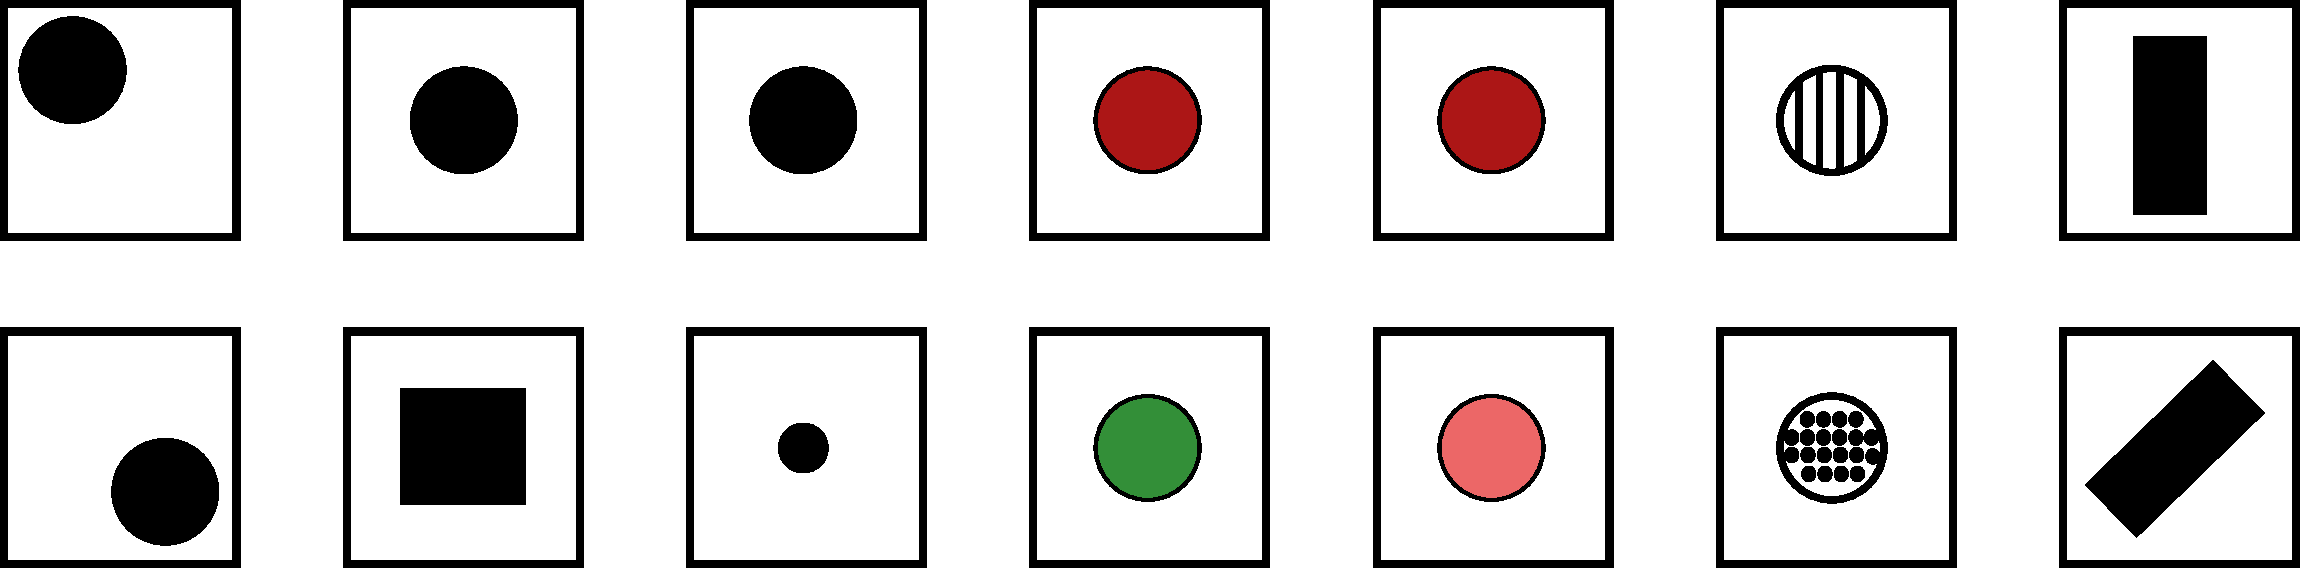
\includegraphics[width=\mycolumnwidth]{Conceptos_basicos/VariablesVisuales.pdf}
\caption{\small Ejemplo de uso de las distintas variables visuales. De izquierda a derecha: posici�n, forma, tama�o, tono, valor, textura, y orientaci�n}
\label{Fig:VariablesVisuales} 
\end{figure}


Todas ellas constituyen las variables visuales, que estudiaremos seguidamente en detalle. El color, como explicaremos, se divide en dos variables visuales independientes: valor y tono.\index{Variables visuales|(}

Las variables visuales se aplican de forma distinta en funci�n del tipo de elemento que queramos simbolizar, por lo que detallaremos su uso para las tres clases de s�mbolos que podemos incorporar en un mapa: puntuales, lineales y de superficie.

\subsection{Posici�n}

La posici�n constituye un caso particular de variable visual a la hora de emplearla en la creaci�n de cartograf�a, ya que viene fuertemente condicionada por el hecho de que todo aquello que representamos tiene una posici�n en el espacio y, por tanto, ha de tener una posici�n concreta en el mapa. Mientras que en cualquier otro tipo de gr�fico la posici�n puede modificarse a voluntad para transmitir alg�n tipo de informaci�n, tal y como haremos con las restantes variables visuales, en el caso de un mapa la posici�n ya est� asociada a una informaci�n que ha de transmitir: la informaci�n sobre la posici�n real en el espacio geogr�fico de aquel objeto que se simboliza.

Aunque el cart�grafo puede en determinadas ocasiones variar la posici�n de algunos elementos (por ejemplo, para mejorar la legibilidad del mapa), siempre est� supeditado a la correcci�n cartogr�fica, y no posee libertad para alterar esta de cualquier modo. Por ello, el uso de la posici�n como variable visual est� muy restringido en el caso de un mapa, y no se emplea. Su escasa aplicaci�n en ese sentido queda patente en el hecho de que en algunos textos no se menciona junto a las restantes variables visuales, detall�ndose por separado como un elemento distinto.


\subsection{Forma}

La forma viene definida por el per�metro exterior del objeto. Esto no implica que �nicamente se pueda aplicar la forma a s�mbolos de superficie, ni tampoco que se debe tratar de un per�metro cerrado como el de una forma poligonal.

La forma se aplica fundamentalmente a los s�mbolos puntuales, situando un s�mbolo de una forma dada sobre las coordenadas exactas del punto a representar. Su aplicaci�n a s�mbolos lineales es dif�cil y no se da, mientras que en el caso de aplicarse sobre s�mbolos de superficie requiere la alteraci�n de los pol�gonos representados (por ejemplo, que tracen los l�mites de pa�ses), dando lugar a una representaci�n imprecisa, al menos en lo que al contorno del pol�gono respecta. Esto se produce �nicamente en el caso de los denominados \emph{cartogramas}, un tipo particular de mapas que veremos en el pr�ximo cap�tulo.

\subsection{Tama�o}

El tama�o se refiere a la dimensi�n del s�mbolo. Para el caso de s�mbolos puntuales, puede aplicarse sin m�s que hacer m�s grande o peque�o el s�mbolo en s�. En el caso de l�neas, el grosor de estas constituye la forma de aplicar la variable tama�o. Al igual que suced�a con la forma, en las superficies va a implicar la modificaci�n de estas, por lo que se emplea �nicamente en los cartogramas. Otra forma de aplicar el tama�o a los s�mbolos superficiales es hacerlo sobre la textura con la que estos se rellenan, usando un �nico patr�n con diferentes tama�os en sus tramas (Figura \ref{Fig:TamanoTexturas}).\index{Cartograma}


\begin{figure}[!hbt]
\centering
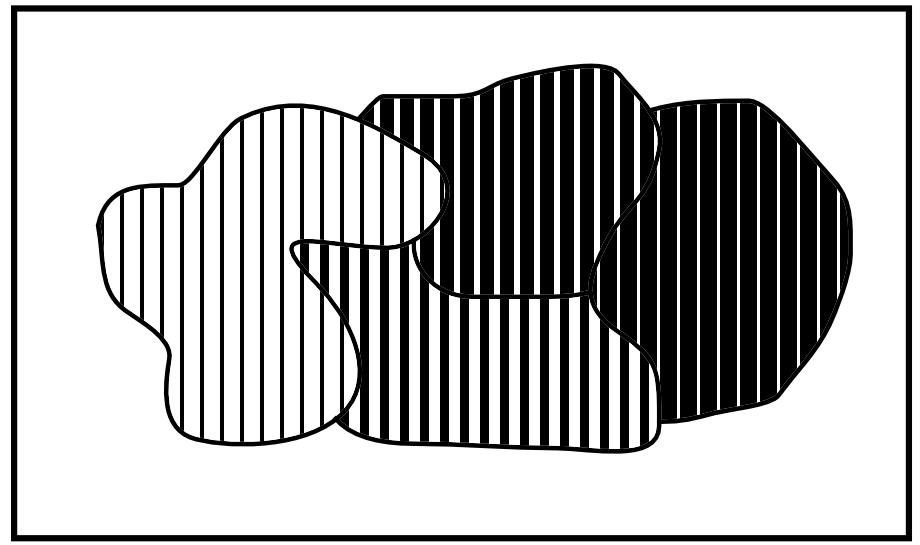
\includegraphics[width=.4\mycolumnwidth]{Conceptos_basicos/Texturas.png}
\caption{\small Uso del tama�o en s�mbolos de superficie mediante texturas.}
\label{Fig:TamanoTexturas} 
\end{figure}


El tama�o condiciona la percepci�n de otras variables visuales, especialmente cuando se trata de tama�os peque�os. Un punto muy peque�o o una l�nea demasiado fina no van a permitir la aplicaci�n de, por ejemplo, el tono o el valor, o al menos no del mismo modo que con un tama�o mayor, ya que la percepci�n de estas variables ser� m�s dif�cil.


\subsection{Color}

La variable color es la m�s importante de todas las variables visuales, y la que a su vez requiere un grado mayor de detalle en su exposici�n, debido a la que complejidad que presenta y a las posibilidades que ofrece\footnote{Si estas leyendo una copia impresa de este libro, es posible adquirir esta tanto en versi�n a color como en versi�n en blanco y negro. En caso de usar esta �ltima, no vas a poder apreciar correctamente algunas de las im�genes de este cap�tulo, por lo que te recomiendo acudir a la versi�n digital del libro (recuerda, este es un libro libre y puedes obtener esa versi�n de forma gratuita en el p�gina Web del libro), al menos para este cap�tulo, o, mejor a�n, para toda esta parte dedicada a la visualizaci�n. Otros cap�tulos en otras partes del libro tambi�n presentan figuras en color, pero pueden ser interpretadas igualmente en blanco y negro. En las de este, no obstante, el uso del color es m�s relevante y ser� mejor utilizar una versi�n con figuras a todo color, ya sea impresa o digital.}.

Existen muchas formas de representar y crear un color, a trav�s de los denominados \emph{espacios de color}. De cara a su uso como variable visual en el contexto de este cap�tulo, resulta de especial inter�s el uso del espacio de color HSV, en el cual un color se define mediante un espacio de coordenadas cil�ndrico, seg�n lo mostrado en la figura \ref{Fig:HSV}. \index{Espacio de color} \index{Espacio de color HSV}

\begin{figure}[!hbt]
\centering
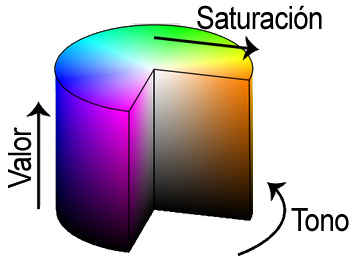
\includegraphics[width=.4\mycolumnwidth]{Conceptos_basicos/HSV.png}
\caption{\small Espacio de color HSV explicando el significado de las componentes tono, valor y saturaci�n (adaptado de Wikipedia).}
\label{Fig:HSV} 
\end{figure}

Tres son las componentes de un color, las cuales establecen sus coordenadas en el cilindro: tono, valor y saturaci�n.

El tono es lo que en el lenguaje com�n denominar�amos color, es decir el nombre del color, por ejemplo verde, rojo o amarillo. Est� relacionado con la longitud de onda de la luz, y distintas longitudes de onda producen un efecto perceptivo distinto, haciendo que distingamos as� los diferentes colores. En el cilindro del espacio de color, el tono viene marcado por el �ngulo del vector definido por la posici�n del color y el eje central, sobre el plano perpendicular a dicho eje.

El tono puede verse alterado por los tonos del entorno, especialmente en s�mbolos de peque�o tama�o. Aunque es una variable para la que la percepci�n humana tiene gran sensibilidad, en los s�mbolos peque�os puede ser dif�cil de identificar y pueden producirse una falsa percepci�n si comparten espacio con otras m�s grandes de un tono distinto. Por ejemplo, al trazar una linea con un grosor fino que atraviesa una serie de pol�gonos de distintos colores, el tono de esta se percibir� como distinto en cada uno de esos pol�gonos por el efecto que sus colores causan como colores de fondo.

Por su parte, el valor indica la claridad del color. Un tono azul puede ser m�s claro o m�s oscuro sin dejar de ser azul. Esa variaci�n que se produce es una variaci�n del valor del color. En el caso de usar una tinta de un color dado, la mezcla de esta con una pintura blanca produce una disminuci�n del valor, aclar�ndose progresivamente seg�n a�adimos m�s de esta �ltima en la mezcla. A la hora de imprimir se hace uso de tramas m�s o menos densas para modificar el valor, sin modificar as� la tinta. Seg�n el espacio en blanco que se deja entre los puntos de tinta impresos, se consigue la apariencia de un color de mayor o menor valor. El valor se define en el cilindro de coordenadas como la altura del color sobre el eje central.

La capacidad de diferenciar dos s�mbolos con valor distinto var�a en funci�n del tipo de s�mbolo. As�, es mayor en el caso de s�mbolos de superficie, mientras que en el caso de s�mbolos puntuales y lineales est� relacionada con el tama�o. Si el punto es muy peque�o o la l�nea muy delgada, es m�s dif�cil apreciar el valor y, por tanto, comparar este con otro o extraer la informaci�n que mediante esa variable visual se intenta transmitir.

La saturaci�n, por �ltimo, expresa la pureza relativa del color. Depende del n�mero de distintas longitudes de onda que aparecen en un color dado. A medida que disminuye la saturaci�n, el color va pareciendo m�s gris�ceo, y el n�mero de longitudes de onda es mayor. En el cilindro del espacio de color queda definido por la distancia del color al eje central.

En lo que al color como variable visual respecta, cada una de estas componentes de un color son a su vez variables visuales, y como tales pueden emplearse para simbolizar los distintos elementos de un mapa. En la pr�ctica, el tono y el valor son utilizadas muy frecuentemente, pero la saturaci�n tiene una utilidad muy limitada, por lo que es muy infrecuente su uso. En lo sucesivo, por tanto, trataremos el color no como una �nica variable visual sino como dos distintas: valor y tono.

Si tienes un programa de dibujo o de edici�n de im�genes, puedes experimentar construyendo colores seg�n sus componentes, usando el habitual selector de colores. Si no, prueba en la siguiente direcci�n Web, donde encontrar�s un selector de colores \emph{on--line}: \url{http://www.dgx.cz/tools/colormixer/stripe.php?hsv=space\%20color}.

La figura \ref{Fig:SelectorColores} muestra el aspecto de un selector de colores, en el que puede verse c�mo estos pueden definirse mediante sus componentes tono (H), saturaci�n (S) y luminosidad (L). Aunque no es exactamente el mismo concepto, la luminosidad cumple el papel del valor en este contexto, y este modelo (HSL en lugar de HSV) es el que encontramos con car�cter habitual en las herramientas de este tipo para definir un color.

\begin{figure}[!hbt]
\centering
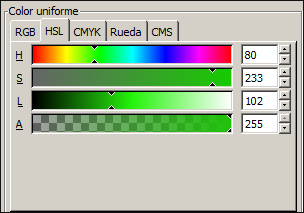
\includegraphics[width=.4\mycolumnwidth]{Conceptos_basicos/SelectorColores.png}
\caption{\small Selector de colores mediante sus componentes tono (H), saturaci�n (S) y luminosidad (L). La componente de la parte inferior es la denominada \emph{alpha}, que indica la transparencia del color.}
\label{Fig:SelectorColores} 
\end{figure}


\subsection{Textura}

La textura hace referencia al relleno de un s�mbolo mediante alg�n patr�n. Empleando patrones distintos se produce una diferenciaci�n en los s�mbolos correspondientes. 

En el caso de los s�mbolos puntuales, la textura requiere que estos tengan un tama�o suficiente para que pueda apreciarse el patr�n que constituye cada una de las texturas. Este tama�o m�nimo requerido es mayor que en el caso de emplear el tono o el valor.

En el caso de l�neas, entendemos como textura el uso de guiones y espacios en blanco que dan lugar a un patr�n de discontinuidad, como se muestra en la figura \ref{Fig:Texturas}.  No obstante, esta discontinuidad es una desventaja a la hora de representar un elemento lineal, ya que implica que una parte de �l no va a representarse. Dependiendo del significado de aquello que representemos, el uso de texturas en elementos lineales puede no ser lo m�s recomendable a la hora de crear un mapa. Puede emplearse otro tipo de texturas para formar l�neas, <<rellenando>> estas si tienen un grosor considerable, pero su uso no se recomienda.

Las texturas se aprovechan plenamente sobre los s�mbolos de superficie, ya que la mayor dimensi�n de estos permite una percepci�n completa y una interpretaci�n mucho m�s sencilla, al igual que ocurr�a en el caso del valor.

\begin{figure}[!hbt]
\centering
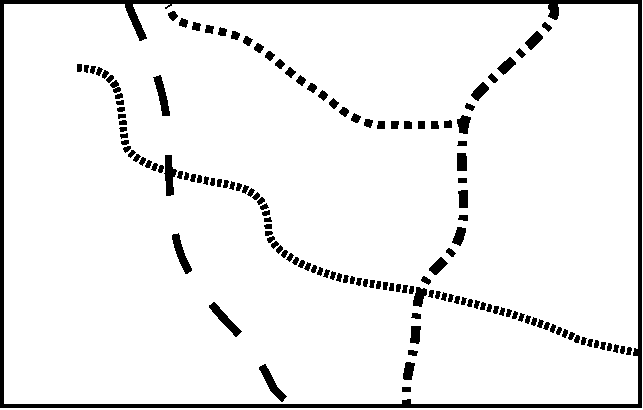
\includegraphics[width=.5\mycolumnwidth]{Conceptos_basicos/Texturas.pdf}
\caption{\small Aplicaci�n de la variable visual textura a los s�mbolos lineales.}
\label{Fig:Texturas} 
\end{figure}


\subsection{Orientaci�n}

La �ltima variable visual es la orientaci�n. Se aplica sobre los s�mbolos puntuales, siempre que estos no presenten simetr�as que impidan percibir correctamente la orientaci�n. Por ejemplo, para el caso del c�rculo, resulta obvio que no tiene sentido aplicar la orientaci�n como variable visual. Los s�mbolos compuestos por formas geom�tricas son adecuados para emplear la orientaci�n, mientras que los s�mbolos pict�ricos no responden de igual forma y producen en la representaci�n sensaci�n de desequilibrio. Se recomienda, por tanto, emplear esta variable �nicamente con los primeros.

Puede aplicarse tambi�n sobre los s�mbolos de superficie a trav�s de la textura, variando la orientaci�n de esta. Sobre las l�neas, no obstante, su aplicaci�n no es posible. Puede emplearse en caso de l�neas con textura, pero esto requiere un ancho excesivo para una correcta percepci�n.

\section{Las propiedades de las variables visuales}

Las variables que acabamos de ver son ahora nuestras herramientas que emplearemos para simbolizar la informaci�n geogr�fica y sabemos ya c�mo aplicarlas. Lo que no hemos visto a�n es qu� capacidades tienen y qu� podemos simbolizar mediante ellas, y este es realmente el aspecto clave sobre el que deberemos decidir posteriormente cuando nos dispongamos a crear un mapa, para as� seleccionar la variable visual m�s adecuada en funci�n de aquello que queramos representar.

Se distinguen 4 propiedades b�sicas que una variable visual puede presentar:

\begin{itemize}
	\item Asociativa. Una variable visual presenta la propiedad asociativa si al ser aplicada no aumenta ni disminuye la visibilidad de un elemento. Es decir, cuando en funci�n de esa variable visual no puede asign�rsele m�s o menos importancia a este.
	\item Selectiva. La propiedad selectiva la presentan aquellas variables visuales que, al ser aplicadas, generan distintas categor�as de s�mbolos.
	\item Ordenada. Cuando una variable visual puede emplearse para representar un orden, se dice que presenta la propiedad ordenada.
	\item Cuantitativa. Cuando, adem�s del orden, una variable puede mostrar cantidades o proporciones, entonces se dice que posee la propiedad cuantitativa.
\end{itemize}

\index{Variables visuales!propiedades}

El orden en que se han presentado estas propiedades no es casual, ya que est�n ordenadas dando lugar a lo que Bertin denomina \emph{niveles de organizaci�n}. La propiedad asociativa se sit�a en el nivel m�s bajo, mientras que la cuantitativa ocupa el m�s alto. El nivel de organizaci�n de las variables visuales tiene importancia a la hora de combinar varias de ellas en un s�mbolo, como veremos m�s adelante. Asimismo, y como detallaremos en el cap�tulo siguiente, el nivel de organizaci�n define qu� tipo de informaci�n podemos transmitir con una variable visual.\index{Niveles de organizaci�n}

Para ver m�s exactamente el significado de estas propiedades, estudiemos con detalle la figura \ref{Fig:PropiedadesVariablesVisuales}, que muestra diferentes representaciones de un conjunto de s�mbolos (en este caso, s�mbolos puntuales) en los que en cada caso se ha utilizado �nicamente una variable visual.

\begin{figure}[!hbt]
\centering
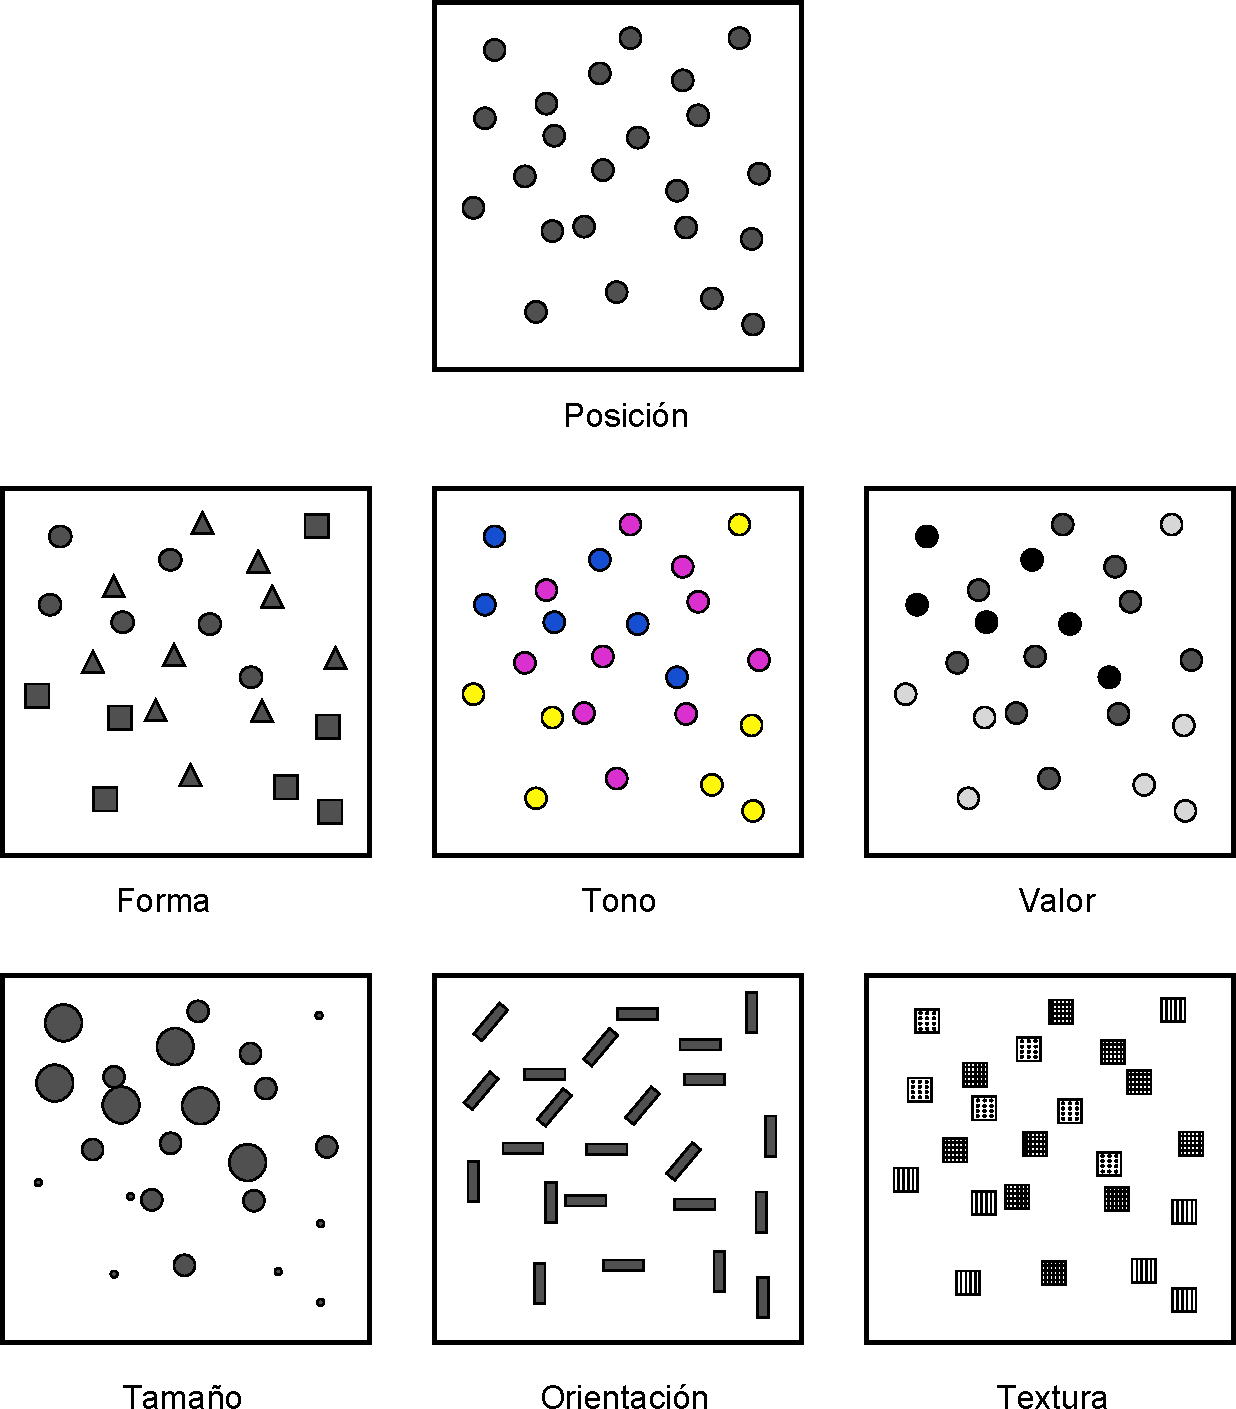
\includegraphics[width=\mycolumnwidth]{Conceptos_basicos/PropiedadesVariablesVisuales.pdf}
\caption{\small Representaci�n de un conjunto de s�mbolos aplicando de forma individual las distintas variables visuales.}
\label{Fig:PropiedadesVariablesVisuales} 
\end{figure}

Comenzando con la propiedad asociativa, vemos que a excepci�n del tama�o y el tono, las dem�s variables visuales no hacen que los elementos presenten una preponderancia en la imagen. No existen una orientaci�n que podamos definir como m�s importante, ni tampoco un color. Lo mismo sucede con la textura, la forma y la posici�n. Podemos emplear una u otra forma, o una u otra textura, y con ello no conseguiremos llamar m�s la atenci�n sobre un elemento en cuesti�n. 

Con el tama�o, sin embargo, resulta claro que mayor tama�o implica un papel destacado dentro de la informaci�n que transmite el mapa. De igual modo, un mayor valor (un color m�s oscuro) da sensaci�n de mayor definici�n, y centra la atenci�n de observador sobre el elemento de un modo muy superior a como lo hace un valor bajo.

Respecto a la propiedad selectiva, diremos que una variable visual la presenta si de un vistazo podemos r�pidamente seleccionar los elementos que pertenecen a un determinado grupo, identificados estos mediante dicha variable visual. El caso m�s claro de propiedad selectiva lo presenta el tono. Podemos r�pidamente quedarnos solo con los elementos amarillos o con los rojos. Aunque no de un modo tan claro, todas las restantes variables presentan igualmente esta propiedad, a excepci�n de la forma. La forma no permite que los elementos se agrupen de modo espont�neo en familias, y su validez en este sentido est� muy ligada a la complejidad de dicha forma.

La propiedad ordenada la presentan aquellas variables que permiten establecer un orden. Tan solo posici�n, textura, tama�o y valor la presentan, mientras que las dem�s carecen de ella. Por ejemplo, en la imagen correspondiente a la variable visual tono no podemos decir cu�les de los elementos situar�amos al principio y cu�les al final de una escala dada definida por esos tonos. Con el valor, sin embargo, s� que podemos, ya que esta escala ir�a de los tonos m�s claros a los m�s oscuros, y visualmente podemos sin dificultad distinguir los distintos niveles y ordenarlos.

Por �ltimo, la propiedad cuantitativa la presentan aquellas variables visuales que permiten estimar proporciones o cantidades de forma visual. Esta propiedad es exclusiva del tama�o y de la posici�n, mientras que las dem�s no la presentan. Podemos visualmente estimar una distancia en comparaci�n con otra y decir que es, por ejemplo, el doble de esta. Tambi�n podemos ver que los c�rculos grandes en la figura correspondiente son aproximadamente el doble que los peque�os. 

El valor, que ya sabemos que presenta la propiedad ordenada, podr�a pensarse que tambi�n presenta la propiedad cuantitativa, pero no sucede as�. Es dif�cil e impreciso afirmar que un color es el doble de oscuro que otro, y lo m�s que podemos hacer es situarlo entre dos valores distintos (de ah� que posea la propiedad ordenada), pero no deducir una cifra que exprese una cantidad o proporci�n. Las restantes variables visuales resulta claro que no poseen esta propiedad.

En el cuadro \ref{Tabla:PropiedadesVariablesVisuales} se muestra un resumen de todo lo anterior.

\begin{table}[!hbt]
\small
\centering  \label{Tabla:PropiedadesVariablesVisuales}
\begin{tabular}{p{3.6cm}ccccccc}  
 & \rotatebox{60}{\textbf{Posici�n}} & \rotatebox{60}{\textbf{Tama�o}} & \rotatebox{60}{\textbf{Forma}} & \rotatebox{60}{\textbf{Valor}} & \rotatebox{60}{\textbf{Tono}} & \rotatebox{60}{\textbf{Textura}} & \rotatebox{60}{\textbf{Orientaci�n}} \\ \midrule   
\textbf{Asociativa}& $\diamondsuit$ & - & $\diamondsuit$ & - & $\diamondsuit$ & $\diamondsuit$ & $\diamondsuit$ \\
\textbf{Selectiva}& $\diamondsuit$ & $\diamondsuit$ & - & $\diamondsuit$ & $\diamondsuit$ & $\diamondsuit$ & $\diamondsuit$ \\
\textbf{Ordenada}&$\diamondsuit$ & $\diamondsuit$ & - & $\diamondsuit$ & - & - & - \\
\textbf{Cuantitativa}& $\diamondsuit$ & $\diamondsuit$ & - & - & - & - & -  \\
\bottomrule \end{tabular}
\caption{\small Cuadro resumen con las propiedades de las variables visuales.}
\end{table}


Aunque las ideas de Bertin conforman una s�lida base te�rica de reconocido valor, lo cierto es que debe permitirse cierta laxitud en la aplicaci�n de estas, y no considerar que existe una dicotom�a estricta en el caso de las propiedades antes presentadas. Hay muchos factores y circunstancias que pueden alterar la forma en que estas propiedades se presentan, y alterar la intensidad con que aparecen en unas u otras variables visuales. Por ejemplo, aunque el tono no presenta, seg�n la propuesta original de Bertin, la propiedad ordenada, s� que puede emplearse para representar un orden en determinadas circunstancias. Si estamos simbolizando unos valores de temperatura, podemos establecer una transici�n de colores entre el rojo y el azul, que ser�n f�cilmente identificados y ordenados por el observador del mapa, ya que el primero de estos colores se asocia habitualmente al calor y el segundo al fr�o. En este contexto particular, el tono s� presenta la propiedad ordenada. En los cap�tulos \ref{Algebra_de_mapas} o \ref{Creacion_capas_raster} ver�s muchos ejemplos de representaciones en que se usan gradaciones de tono para simbolizar variables de tipo cuantitativo, ya sean razones o proporciones. Estas guardan, no obstante, cierta l�gica, de tal modo que puede entenderse adecuadamente su significado. Como veremos en el pr�ximo cap�tulo, esto tambi�n tiene relaci�n con el tipo de mapa, de tal modo que ciertos tipos de mapas permiten por sus propias caracter�sticas el uso del tono para este tipo de variables.

Junto a lo anterior, algunos autores (v�ase \cite{MacEachren2004Guilidford}) expanden el n�mero de variables visuales y se han desarrollado revisiones a las propiedades enunciadas por Bertin basadas en estudios pr�cticos, que demuestran c�mo pueden existir variaciones sobre la relaci�n entre estas y las distintas variables visuales (por ejemplo, \cite{TreiSman1988PR}).

\section{Uso combinado de las variables visuales}

Para explicar cada una de las variables visuales, hemos visto diversos ejemplos en los que utiliz�bamos cada una de ellas por separado y de forma �nica. Sin embargo, las variables visuales pueden combinarse y, si se hace de la manera correcta, esto reforzar� la capacidad que estas tienen para transmitir una informaci�n dada. La imagen \ref{Fig:CombinacionVariablesVisuales} muestra algunos ejemplos de combinaci�n de variables visuales que nos servir�n para detallar la forma adecuada de usas varias de ellas simult�neamente.

\begin{figure}[!hbt]
\centering
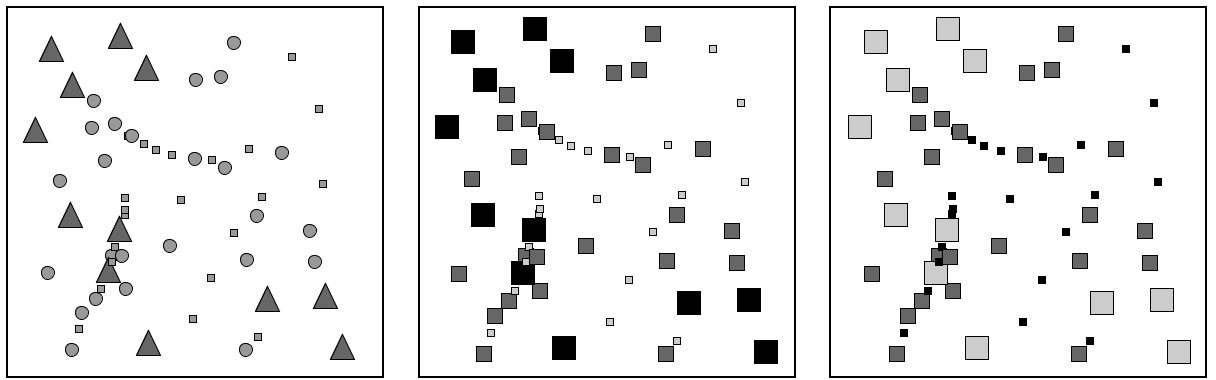
\includegraphics[width=\mycolumnwidth]{Conceptos_basicos/CombinacionVariablesVisuales.png}
\caption{\small Combinaci�n de variables visuales.}
\label{Fig:CombinacionVariablesVisuales} 
\end{figure}

\index{Variables visuales!uso combinado}

El primero de los ejemplos propuestos muestra el uso combinado de las variables tama�o y forma para s�mbolos puntuales. Estos s�mbolos representan la profundidad del suelo medida en determinados emplazamientos, estando relacionado un mayor tama�o del s�mbolo  con una profundidad mayor. Asimismo, se ha asociado un s�mbolo triangular a los valores m�s bajos, un s�mbolo circular a los intermedios y uno cuadrado a los m�s altos. Aunque se emplean dos variables visuales distintas, el resultado no es, sin embargo, mejor que en caso de emplear uno solo de ellos (en este caso, deber�a emplearse el tama�o, ya que la forma no presenta la propiedad cuantitativa necesaria para representar cantidades). Lejos de producirse una sinergia entre el efecto de ambas variables, el resultado es similar al uso exclusivo del tama�o en cuanto a su capacidad de transmitir la informaci�n, o incluso peor, ya que la forma puede dificultar la estimaci�n visual del tama�o, al ser m�s complicado comparar la dimensi�n de objetos de distinta forma.

Pese a que no es clara la ventaja de aplicar conjuntamente las variables forma y tama�o, esta puede emplearse para representar cantidades, por lo que podemos decir que mantiene la propiedad cuantitativa que posee el tama�o. En general, al combinar dos variables visuales el resultado presentara las propiedades de aquella que tenga un mayor nivel organizativo. Puesto que la propiedad cuantitativa representa el nivel organizativo superior, en este caso se mantiene en la combinaci�n.

A�n as�, hay mejores formas de combinar las variables visuales para que esta combinaci�n enfatice en mayor grado la informaci�n que se pretende transmitir, como por ejemplo la mostrada en el segundo ejemplo. Este ejemplo combina el tama�o y el valor, variables ambas que no poseen la propiedad asociativa. Es decir, poseen su complementaria, que podr�amos denominar \emph{disociativa}, y que, recordemos, es la propiedad que, al aplicarse sobre un s�mbolo, hace que este gane importancia visual. El resultado presenta un car�cter todav�a m�s disociativo, en cuanto que los s�mbolos que representan una cantidad elevada, al ser no solo grandes, sino estar pintados en color oscuro, llaman a�n m�s nuestra atenci�n que si emple�ramos una �nica de las variables visuales utilizadas.

Como regla en este sentido, podemos decir que, cuando se combinan variables visuales que poseen una determinada propiedad, en el resultado esta propiedad queda reforzada con respecto a las variables individuales.

El tercer ejemplo nos muestra que combinar variables visuales con una misma propiedad no garantiza necesariamente que se vaya a producir una sinergia entre ellas, sino que, por el contrario, pueden anularse. Las variables empleadas en este caso son las mismas, valor y tama�o, pero se ha asociado el color claro a los valores mayores y el oscuro a los menores, de tal modo que los s�mbolos de mayor tama�o son m�s claros que los peque�os. Esto aten�a el efecto disociativo del tama�o, de forma que la representaci�n es m�s dif�cil de interpretar y su informaci�n no se transmite de modo tan inmediato y directo.

En resumen, podemos sintetizar lo anterior diciendo que, a la hora de combinar variables visuales, deben tenerse en cuenta las propiedades de estas del mismo modo que cuando se emplean de forma individual. Las propiedades a reforzar ser�n aquellas que convengan m�s al tipo de informaci�n representado, y deben presentarlas todas las variables a combinar para que el efecto conjunto sea m�s acusado.


\section{La percepci�n visual}

La percepci�n engloba toda la serie de procesos que convierten un fen�meno f�sico en una informaci�n acerca de nuestro entorno, a trav�s de la estimulaci�n de unos �rganos perceptivos. La percepci�n tiene una fase f�sica, una fisiol�gica (la estimulaci�n en s�) y una psicol�gica (la interpretaci�n del est�mulo). En el caso de la percepci�n visual, este fen�meno f�sico es de tipo energ�tico (la luz), y los �rganos correspondientes son los ojos. \index{Percepci�n visual}

El estudio de la percepci�n es un fen�meno complejo que no entraremos a detallar, pero en el que resulta de inter�s profundizar para conocer algo m�s acerca de c�mo la informaci�n que plasmamos en un mapa (que es un elemento visual) acaba convertida en una informaci�n en la mente del observador de ese mapa. Entender este proceso, al menos someramente, nos permitir� mejorar la eficacia de la percepci�n, de forma que tengamos una mayor garant�a de que la informaci�n que transmitimos sea recibida e interpretada correctamente.

Dos son los aspectos que detallaremos en esta secci�n: las constancias perceptivas y las ayudas a la percepci�n. En otras palabras, hasta qu� punto podemos modificar los elementos visuales o su entorno sin que dejen de transmitir su informaci�n y sean confundidos sus caracter�sticas, y c�mo podemos facilitar que se perciban exactamente como pretendemos.

\subsection{Las constancias y contrastes perceptivos}

Entendemos por constancias perceptivas a las propiedades de los objetos cuya percepci�n no var�a aunque se produzcan modificaciones. Podemos ver algunos ejemplos para algunas de las variables visuales que conocemos.

\index{Constancia perceptiva}\index{Contraste perceptivo}

Dado un objeto redondo tal como una rueda, si lo miramos en una direcci�n perpendicular aparecer� efectivamente como una forma circular perfecta. Sin embargo, si la miramos desde otro �ngulo, veremos una forma el�ptica, pero ello no nos lleva a pensar que la rueda en s� no sea ya redonda. Nuestra percepci�n de esa rueda es la misma, y podemos apreciar de igual modo su tama�o o su forma. Alterar el �ngulo de visi�n no altera el objeto y la percepci�n que tenemos de �l.

Del mismo modo, un elemento pintado de un color claro se identifica como tal aunque la luz sea tenue, y un elemento oscuro lo seguimos percibiendo como oscuro aunque estemos en unas condiciones de iluminaci�n fuerte. Nuestro cerebro es capaz de interpretar simult�neamente el objeto y el contexto, y de este modo extraer las caracter�sticas de ese objeto, que no var�an.

Estos dos ejemplos muestran la constancia perceptiva de la forma y el valor, y podemos buscar otros similares para otras variables visuales.

No todas las variables visuales tienen una constancia perceptiva como la anterior. Todos conocemos m�ltiples ejemplos de ilusiones �pticas en las que algo no parece lo que realmente es, y esa percepci�n err�nea viene normalmente motivada por las condiciones en las que percibimos el objeto, por ejemplo debido al entorno particular en el que este se encuentra junto a otros objetos. La figura \ref{Fig:Zollner} muestra un ejemplo cl�sico de ilusi�n �ptica, conocida como \emph{ilusi�n de Zollner}. Las lineas largas diagonales son paralelas, pero no aparentan serlo, debido al efecto causado por las l�neas m�s cortas. En este caso, no existe una constancia perceptiva de la variable visual orientaci�n.

\index{Ilusi�n de Zollner}

Cuando la percepci�n de un elemento cambia aunque el estimulo no lo haga, en lugar de una constancia perceptiva hablamos de un \emph{contraste perceptivo}. Los contrastes perceptivos son importantes, ya que pueden inducir una interpretaci�n err�nea de la informaci�n que pretendemos transmitir, al producirse una percepci�n equivocada.


\begin{figure}[!hbt]
\centering

\includegraphics[width=.5\mycolumnwidth]{Conceptos_basicos/Zollner_illusion.png}
\caption{\small Ilusi�n de Zollner que demuestra el contraste perceptivo de la orientaci�n.}
\label{Fig:Zollner} 
\end{figure}

Las siguientes son algunas de las ideas m�s importantes a tener en cuenta a este respecto a la hora de crear un mapa:

\begin{itemize}
	\item El tama�o es la variable visual que m�s afectada se ve, y el tama�o aparente de un objeto puede variar notablemente si se encuentra rodeado de otros de un tama�o distinto. La figura \ref{Fig:ContrasteTamano} muestra un ejemplo de esto. A la hora de emplear simbolog�a de elementos puntuales en un mapa (por ejemplo, en un mapa de s�mbolos graduados, como veremos en el apartado \ref{MapasSimbolosGraduados}), esto debe tenerse en cuenta, ya que pueden presentarse situaciones como la de la figura.	
	\item El valor se ve igualmente alterado al situar alrededor elementos de distinto valor. Si el n�mero de distintos valores es peque�o, es m�s dif�cil que aparezca este contraste perceptivo. A medida que se aumenta el n�mero de estos, es m�s probable que aparezca en mayor o menor medida.
	\item El tono se ve alterado por la presencia de otros tonos distintos. En un mapa, veremos este efecto al enfrentar el color de un elemento sobre el color del fondo. Por ejemplo, si una l�nea que representa a una carretera y cruza una serie de pol�gonos de distinto tono, puede parecer que el tono de la l�nea varia aunque en realidad sea constante.
	\item Tonos complementarios puestos juntos pueden crear sensaci�n de vibraci�n en la frontera que los separa.
\end{itemize}

\begin{figure}[!hbt]
\centering
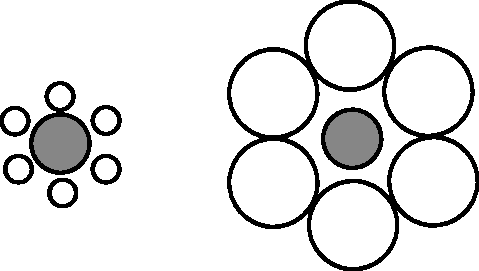
\includegraphics[width=.6\mycolumnwidth]{Conceptos_basicos/ContrasteTamano.pdf}
\caption{\small Contraste perceptivo del tama�o. Ambos circulos grises tienen el mismo tama�o, pero el de la izquierda aparenta ser mayor.}
\label{Fig:ContrasteTamano} 
\end{figure}

\subsection{Ayudas a la percepci�n}\label{AyudasPercepcion}

Con lo que hemos visto anteriormente, queda claro que podemos alterar la forma en que se perciben las variables visuales que caracterizan a un elemento visual. Podemos usar este hecho para nuestro beneficio, de tal modo que el dise�o de un mapa incorpore elementos que hagan m�s patente la informaci�n que este contiene, facilitando la correcta percepci�n del mapa en su conjunto.

Un factor clave en este sentido es la adecuado separaci�n entre el fondo y la figura. Aquello que queremos que resulte visible con car�cter principal (en el caso de un mapa, sus distintos elementos) debe separarse de aquello que constituye el fondo de la imagen, y debe atraer la atenci�n del observador de manera prioritaria. En caso de no ser as�, puede resultar dif�cil <<descubrir>> la informaci�n que el mapa transmite, al quedar esta al mismo nivel que la de otros elementos de menor importancia. El ejemplo cl�sico de la figura \ref{Fig:CupOrFaces} ilustra este hecho. Puesto que no existe una diferenciaci�n clara entre el fondo y la figura, no es obvio saber si la imagen pretende representar una copa o dos caras.

\begin{figure}[!hbt]
\centering

\includegraphics[width=.35\mycolumnwidth]{Conceptos_basicos/Cup_or_faces_paradox.pdf}
\caption{\small Sin un adecuado contraste entre fondo y figura la imagen presenta ambig�edad.}
\label{Fig:CupOrFaces} 
\end{figure}

En un mapa, y como veremos en el pr�ximo cap�tulo, encontramos dos tipos de cartograf�a: una con car�cter de base que define un contexto geogr�fico, y una tem�tica que constituye la informaci�n principal que se transmite con el mapa. Puesto que esta segunda es la fundamental y de mayor importancia, y la primera se incluye tan solo como apoyo de esta, es importante asegurarse de que esa cartograf�a base no interfiere y se mantiene en un segundo plano, constituy�ndose como fondo y dejando que sea la informaci�n tem�tica la que act�e como figura. Para ello podemos emplear las distintas variables visuales aplicadas a la cartograf�a base, de modo que su importancia relativa no sea mayor que la de los elementos principales de la parte tem�tica.

Otro aspecto a considerar es la adecuada jerarquizaci�n entre los elementos del mapa. La divisi�n entre fondo y figura ya constituye en s� una jerarquizaci�n, pero no es suficiente si conviven varios tipos de elementos en el mapa. Dentro de la parte tem�tica es necesario estructurar estos visualmente para que quede clara su importancia y se vea sin dificultad que existe una divisi�n entre ellos.\index{Jerarquizaci�n}\index{Fondo--figura}

Esta jerarqu�a debe aportar una <<profundidad>> a la informaci�n, de forma que existan niveles en esta y se perciba que algunos elementos est�n por encima de otros. Como veremos en el cap�tulo \ref{Visualizacion_SIG}, la forma de ordenar las distintas capas en un SIG ya establece un orden, aunque este no es en s� suficiente, y deben utilizarse las variables visuales para enfatizar o no unas o otras capas y la informaci�n que contienen.

Algunas t�cnicas b�sicas para esto son las que permiten que exista alg�n factor diferencial en la informaci�n m�s relevante. Si las propiedades de los elementos destacados difieren notablemente de las del fondo, esto centra la atenci�n sobre ellas y garantiza que no se confundan con este. Emplear unas caracter�sticas m�s homog�neas para el fondo permite que la diferenciaci�n de la figura sea m�s patente. En otras palabras, el contraste, aplicado este a todas las variables visuales, es una de las claves para lograr una adecuada transmisi�n de la informaci�n al emplear una representaci�n visual.

El contraste se aplica no solo a las variable visuales, sino en general a las caracter�sticas de la representaci�n. Por ejemplo, el nivel de detalle es una propiedad susceptible de ser utilizada para enfatizar algo. As�, y en el caso particular del documento cartogr�fico, el lector de un mapa espera que el detalle sea mayor en la cartograf�a tem�tica que en la de base, ya que esta �ltima es simplemente un elemento complementario de ayuda. Un mayor detalle sobre ciertos elementos llamar� m�s la atenci�n en contrate con un fondo menos detallado, y esto puede utilizarse para enfocar la atenci�n sobre lo m�s relevante. Ofrecer menos detalle en la cartograf�a de base no es un inconveniente si esto ayuda a un mejor entendimiento de los elementos principales del mapa.

Como ejemplo de lo anterior, la figura \ref{Fig:JerarquiaMapa} muestra un ejemplo de como una correcta jerarquizaci�n es fundamental para crear mapas de calidad.

\begin{figure}[!hbt]
\centering
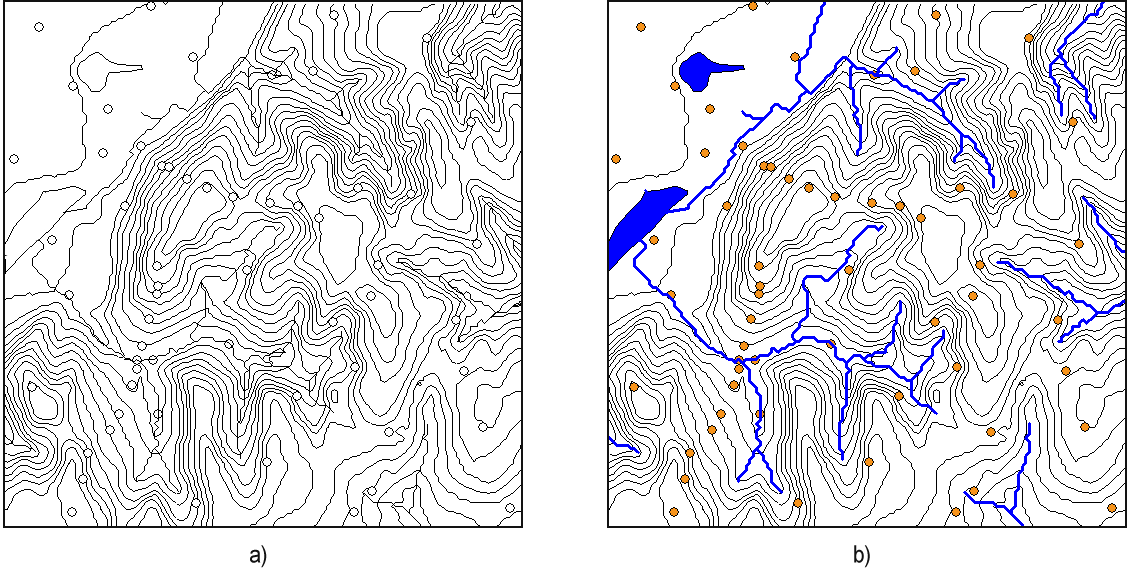
\includegraphics[width=.9\mycolumnwidth]{Conceptos_basicos/JerarquiaMapa.png}
\caption{\small Mapa con jerarqu�a incorrecta (a) y mapa adecuadamente jerarquizado (b).}
\label{Fig:JerarquiaMapa} 
\end{figure}

Por �ltimo, un aspecto clave para la claridad de un mapa es el relativo al poder separador. Este define la capacidad de un individuo para distinguir objetos muy peque�os y separar objetos cercanos. Adem�s de depender del propio individuo, est� condicionado por una serie de factores. 

Se admite en l�neas generales que el l�mite de separaci�n entre dos objetos para el ojo humano es de 0,2mm. Si existe una distancia menor entre ellos, en condiciones normales no ser� posible distinguir uno de otro. \index{Limite@L�mite de separaci�n}

Existe tambi�n un l�mite para poder reconocer objetos aislados, aunque este depende del tipo de objeto. Los siguientes son algunos de los aplicados usualmente:

\begin{itemize}
	\item 0,2mm de diametro para el caso de un punto.
	\item 0,5mm de grosor para el caso de una l�nea negra.
	\item 0,4mm de lado para el caso de un cuadrado negro.
	\item 0,6mm de lado para un cuadrado sin relleno.
\end{itemize}

Existe asimismo un umbral de diferenciaci�n, que define el tama�o m�nimo de dos objetos para que puedan ser percibidos como distintos. Este umbral tambi�n depende de las caracteristicas de los objetos, como por ejemplo la forma (si las formas son muy distintas ser� m�s f�cil distinguirlos que si son muy similares). 

El poder separador no depende �nicamente de variables de tipo espacial, sino que tambi�n est� en relaci�n con otras variables visuales. Por ejemplo, una l�nea negra sobre fondo blanco puede distinguirse aunque sea fina, pero en caso de ser amarilla sobre ese mismo fondo, ser� necesario un grosor mayor.

Como parece l�gico, estos conceptos deben usarse para no incorporar a un mapa elementos que est�n m�s all� del umbral de separaci�n del lector del mapa, ya que en este caso no podr� extraer la informaci�n que se ha incorporado en este al crearlo.

\index{Variables visuales|)}

\section{Resumen}

Para transmitir correctamente cualquier tipo de informaci�n mediante el lenguaje visual, es necesario conocer sus elementos y saber emplearlos de modo adecuado. La semiolog�a gr�fica se encarga del estudio de los s�mbolos del lenguaje visual, y en este cap�tulo hemos visto algunas de sus ideas principales.

De especial relevancia resultan las denominadas \emph{variables visuales}, las cuales empleamos para la caracterizaci�n de s�mbolos. Existen seis variables visuales: posici�n, forma, tama�o, color, textura y orientaci�n. El color a su vez se puede dividir en tres: tono, valor y saturaci�n. De estas tres, solo las dos primeras, tono y valor, tienen aplicaci�n pr�ctica en el �mbito cartogr�fico.

Las variables visuales presentan distintas propiedades, que definen a su vez los \emph{niveles de organizaci�n}. De menor a mayor organizaci�n, estas propiedades son las siguientes: asociativa, selectiva, ordenada, cuantitativa. Las propiedades de una variable visual condicionan el tipo de informaci�n que puede transmitirse haciendo uso de ella. Cuando se combinan varias variables visuales que poseen una misma propiedad, esta propiedad se presenta con mayor fuerza en el resultado.

Podemos ayudar a que la percepci�n de la informaci�n que transmitimos con un elemento visual sea mejor, atendiendo a aspectos como el contraste entre el fondo y la figura, as� como estableciendo una correcta jerarquizaci�n entre los distintos elementos. Igualmente, debemos prestar atenci�n a los contrastes perceptivos, para evitar que estos aparezcan y se produzca una percepci�n incorrecta.



\chapter{El mapa y la comunicaci�n cartogr�fica}\label{El_Mapa}

\begin{keypoints}
�C�mo se produce la comunicaci�n cartogr�fica? $\bullet$ �Qu� es el proceso cartogr�fico? $\bullet$ �Qu� es un mapa? $\bullet$ �De qu� bases se compone? $\bullet$ �Qu� elementos tiene un mapa? $\bullet$ �Qu� se ha de considerar a la hora de crearlo? $\bullet$ �Qu� tipos de mapas hay? $\bullet$ �Qu� caracteriza a cada tipo?\end{keypoints}

\bigskip

\begin{intro}
Dentro o fuera del SIG, el mapa es el medio por excelencia para transmitir la informaci�n geogr�fica de modo visual. Ser capaz de crear representaciones �ptimas durante el trabajo con un SIG implica ser capaz de entender c�mo crear un mapa y saber escoger qu� tipo de mapa es el m�s adecuado en funci�n de la informaci�n a mostrar. En este cap�tulo estudiaremos todo lo relativo a los mapas y sus conceptos fundamentales, as� c�mo las consideraciones necesarias a la hora de crearlos, con objeto de poder abordar en el siguiente el trabajo directo de visualizaci�n dentro de un SIG y analizar qu� aporta este al concepto cl�sico de mapa.

Para seguir este cap�tulo es necesario haber estudiado el cap�tulo anterior, ya que haremos uso de las ideas entonces presentadas acerca de las variables visuales. Algunos conceptos relativos al dise�o cartogr�fico han aparecido ya en cap�tulos previos, por lo que no se repetir�n en este. En particular, el cap�tulo \ref{Fundamentos_cartograficos} dedicado a los fundamentos cartogr�ficos y geogr�ficos contiene materia que debe conocerse antes de abordar la lectura del presente.
\end{intro}


\section{Introducci�n}

Los mapas han sido empleados desde la antig�edad para recoger la informaci�n geogr�fica y transmitirla. Como ya dijimos en el cap�tulo anterior, podemos entender un mapa como un medio de comunicaci�n visual que constituye un lenguaje con un objetivo particular: la descripci�n de relaciones espaciales. Una mapa es, pues, una abstracci�n simb�lica de alg�n fen�meno real, lo cual significa que presenta un cierto grado de simplificaci�n y generalizaci�n.

El dise�o, producci�n y uso de un mapa como forma de comunicaci�n conforma lo que se conoce como \emph{proceso cartogr�fico}. M�s concretamente, el proceso cartogr�fico conlleva cuatro etapas o subprocesos, a saber: \index{Proceso cartogr�fico}

\begin{itemize}
	\item Recoger los datos.
	\item Manipular y generalizar los datos para dise�ar y construir mapas.
	\item Visualizar el mapa.
	\item Interpretar la informaci�n.
\end{itemize}


La labor del cart�grafo se centra en el segundo de estos puntos, mientras que el usuario del mapa lleva a cabo los dos �ltimos. Ser� en esa construcci�n de los mapas en lo que nos fijemos a lo largo de este cap�tulo, para conocer los conceptos y reglas que rigen la comunicaci�n cartogr�fica a trav�s del uso de mapa. El lenguaje visual que estudi�bamos en el cap�tulo \ref{Conceptos_basicos_visualizacion} se convierte ahora en un lenguaje cartogr�fico al adaptarlo al caso particular de la creaci�n de mapas, y estas reglas (equivalentes a la gram�tica y la sintaxis de un lenguaje hablado) son imprescindibles para poder crear cartograf�a que facilite las citadas labores del usuario posterior de esta. Este conjunto de ideas relativas a la producci�n de mapas dan forma a lo que conocemos como \emph{dise�o cartogr�fico}.\index{Dise�o!cartogr�fico}

El dise�o cartogr�fico implica la toma de decisiones por parte del cart�grafo. Algunas de estas decisiones pueden ser la cantidad de simplificaci�n que debe realizarse o los s�mbolos que han de emplearse para plasmar la informaci�n a transmitir. Las ideas desarrolladas en los pr�ximos apartados conforman una base de conocimientos que facilita la toma de decisiones correctas en este sentido.

\section{El prop�sito del mapa}

Como elemento de comunicaci�n, un mapa tiene siempre un prop�sito. De la misma forma que al hablar pretendemos transmitir algo y para ello usamos el lenguaje como herramienta, en el caso de crear un mapa empleamos el lenguaje gr�fico para transmitir una determinada informaci�n geogr�fica. Tambi�n de igual modo que en el caso de la comunicaci�n verbal, y el de cualquier otra forma de comunicaci�n, existe un receptor de nuestro mensaje. Es decir, un usuario (o varios) de ese mapa, que ser�n quienes lo interpreten y aprovechen.

Esto que parece obvio es un hecho en realidad ignorado muchas veces a la hora de elaborar un mapa, y con ello se pierde gran parte de la capacidad del mapa como elemento de comunicaci�n. Aplicar los conceptos de visualizaci�n correctamente, as� como aquellos que veremos en este cap�tulo relativos a la simbolizaci�n, no garantiza que el mapa que generemos sea �til, del mismo modo que aplicar adecuadamente la gram�tica del chino para elaborar una frase no sirve de nada si nuestro interlocutor solo habla castellano, ya que no ser� capaz de interpretar nuestro mensaje por muy correcto que este sea. Resulta incluso mejor elaborar un mensaje con errores gramaticales en castellano, ya que al hacerlo as� estamos teniendo en cuenta las circunstancias en que se produce la comunicaci�n.

Al crear un mapa nunca debemos olvidar qui�n y para qu� va a usar ese mapa, y en funci�n de ello elegir los elementos correctos y la forma de presentar la informaci�n m�s acorde con esos destinatarios y sus objetivos particulares. S�lo entonces es cuando aplicaremos los conceptos del dise�o cartogr�fico para que el mensaje que elaboramos sea el mejor posible.

La figura \ref{Fig:PropositoMapa} muestra un ejemplo claro de lo anterior a trav�s de sendos mapas con predicciones meteorol�gicas, proporcionados por la Agencia Estatal de Meteorolog�a de Espa�a. El primero es un mapa de probabilidad de precipitaci�n, mostrada esta mediante isol�neas. El segundo es un cl�sico mapa del tiempo (conocido como \emph{mapa significativo}) en el que sobre el mismo territorio se sit�an s�mbolos indicando el tiempo previsto (soleado, chubascos, lluvias, tormentas, etc.). Ambos mapas son correctos desde el punto de vista de la labor cartogr�fica y se han creado a partir de una misma informaci�n, pero la forma de mostrar esta es bien distinta. Para un uso cient�fico, este �ltimo mapa resulta claramente insuficiente, mientras que el primero es adecuado. Sin embargo, si la audiencia es no especializada, tal como los lectores de un peri�dico que deseen saber si ma�ana podr�n o no salir al campo a disfrutar de un d�a soleado, el segundo mapa es mucho mejor, ya que el primero, aunque tambi�n proporciona esa informaci�n  e incluso lo hace con m�s detalle, puede resultar excesivamente complejo y dif�cil de entender si no se tienen ciertos conocimientos. Es decir, el usuario es en �ltima instancia, y por encima del propio dise�o cartogr�fico, quien hace que el mapa sea o no un elemento �til.\index{Mapa!significativo}

\begin{figure}[!hbt]
\centering
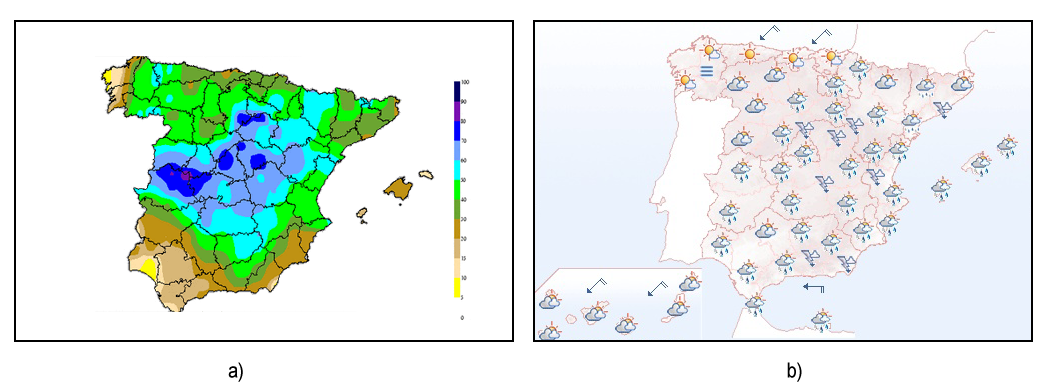
\includegraphics[width=\mycolumnwidth]{Mapas/PropositoMapa.png}
\caption{\small Dos formas distintas de mostrar una informaci�n a trav�s de un mapa. En funci�n del prop�sito de este y el publico al que va dirigido, cada una de ellas podr� ser adecuada o no. (Im�genes cortes�a de AEMET)}
\label{Fig:PropositoMapa} 
\end{figure}


Entre los elementos fundamentales que se han de elegir en funci�n del prop�sito del mapa se encuentran los correspondientes a la base matem�tica del mapa: escala y proyecci�n. La escala condicionar� el tipo de estudios que ser� posible llevar a cabo con el mapa, y establecer� el nivel de detalle que se desea comunicar a trav�s de este (siempre, obviamente, dentro de los limites de la escala a la que se hayan recogido los datos). Por su parte, la proyecci�n debe considerarse en funci�n de sus propiedades. Como ya vimos en el apartado \ref{TiposProyecciones}, toda proyecci�n implica alg�n tipo de distorsi�n. Existen as� proyecciones que mantienen las �reas, las distancias o los �ngulos. Seg�n qu� trabajo se espere con el mapa ser� m�s indicado hacer uso de una u otra de ellas, ya que no es lo mismo un mapa catastral que una carta de navegaci�n, y la elecci�n de una proyecci�n inadecuada puede convertir un mapa en una herramienta in�til para la tarea que se pretende realizar.

El otro aspecto importante a considerar es la forma en que transmitimos la informaci�n a trav�s del mapa, es decir, el tipo de mapa, como hemos visto en el ejemplo propuesto. Dentro de este cap�tulo estudiaremos los tipos de mapas m�s habituales y las caracter�sticas que los definen, as� como la forma de crearlos correctamente.

\section{Cartograf�a tem�tica y cartograf�a base}

Existen muchos tipos de mapas y muchas formas de clasificarlos. Una clasificaci�n especialmente relevante es la que divide a estos en dos grupos cartogr�ficos principales en funci�n del tipo de informaci�n que aporten: \emph{cartograf�a base}, tambi�n denominada \emph{fundamental} o \emph{topogr�fica}, y \emph{cartograf�a tem�tica}.\index{Cartografia!tem�tica y de base}

La cartograf�a base representa el tipo de mapa que originalmente era el objeto principal de la cartograf�a, cuando lo primordial era recoger con precisi�n \emph{qu�} hab�a sobre la Tierra, documentando a trav�s del documento cartogr�fico las caracter�sticas f�sicas de esta. Este tipo de cartograf�a requiere de medidas precisas y se basa fundamentalmente en el trabajo de la topograf�a para obtener la informaci�n necesaria que posteriormente se plasma sobre el mapa.

La cartograf�a base tiene car�cter general, y ello explica que inicialmente fuera el �nico tipo de mapa de inter�s para el cart�grafo, ya que exist�a una indudable necesidad de ese tipo de informaci�n de referencia acerca del entorno f�sico. Una vez que se ha desarrollado una colecci�n suficiente de mapas topogr�ficos y se conoce bien la Tierra a trav�s de ellos, los cart�grafos comienzan a recoger en otro tipo de mapas otras variables espaciales tambi�n susceptibles de ser representadas de ese modo. Esto tiene lugar alrededor del siglo XVIII, y aparece entonces la cartograf�a tem�tica.

La cartograf�a tem�tica se centra en la representaci�n de un tema concreto (una variable espacial dada), pudiendo esta ser de cualquier �ndole: f�sica, social, pol�tica, cultural, etc. Se excluyen de la lista de esos temas posibles a los puramente topogr�ficos, que constituyen el objeto de la cartograf�a base.

La cartograf�a tem�tica se apoya en la cartograf�a base, ya que esta se incluye tambi�n en los mapas tem�ticos para facilitar la comprensi�n del comportamiento espacial de la variable representada y ubicar esta en un contexto geogr�fico dentro del propio mapa. Un mapa tem�tico se compone, as� pues, de dos partes bien diferenciadas:

\begin{itemize}
\item Una capa espec�fica con la informaci�n tem�tica. Contiene la informaci�n principal del mapa, representando la variable espacial sobre la que se construye este.
\item Un mapa base. El mapa base provee una localizaci�n geogr�fica a la que se referencia la informaci�n tem�tica. Debe contener los elementos propios de la cartograf�a base, aunque siempre ha de tenerse en cuenta que estos han de coexistir con los correspondientes a la parte tem�tica. Por ello, frecuentemente es necesario incluir en este mapa base menos detalle que si se dise�ara para ser un mapa independiente, limit�ndose a los elementos necesarios que definan un contexto geogr�fico b�sico. La labor de este mapa base no es ser utilizado como tal como si se tratara de cartograf�a base aislada, sino ayudar a los elementos de la componente  tem�tica a transmitir mejor la informaci�n que contienen.

Aunque en ocasiones puede utilizarse un mapa topogr�fico est�ndar como mapa base, habitualmente este contiene demasiada informaci�n e interfiere con la capa tem�tica, siendo m�s adecuado crear el mapa base a partir de elementos individuales. Algunos de los m�s importantes son el \emph{canev�s} (rejilla de coordenadas, especialmente necesaria a escalas peque�as), la red fluvial, el relieve, la v�as de comunicaci�n, las poblaciones y los nombres geogr�ficos. Todos ellos son buenos elementos de referencia para permitir situar en base a ellos cualquier tipo de informaci�n tem�tica.
\end{itemize}\index{Canev�s}


La mayor�a de las ideas de este y el pr�ximo cap�tulo se aplican fundamentalmente a la cartograf�a tem�tica, siendo esta adem�s la que con mayor frecuencia se genera mediante el uso de un SIG. Una buena parte de lo visto en relaci�n con las variables visuales y sus propiedades tiene mayor relevancia a la hora de tratar con cartograf�a tem�tica, ya que esos conceptos se aplican a la representaci�n de variables y fen�menos de tipo cuantitativo, y es la cartograf�a tem�tica la que trabaja con ellos.

En la cartograf�a topogr�fica, los elementos geom�tricos que representamos son en s� la informaci�n que pretendemos comunicar con el mapa, mientras que en la cartograf�a tem�tica esa geometr�a es solo parte de la informaci�n, siendo la otra parte la que se transmite a trav�s del uso de variables visuales como, por ejemplo, el color. De otro modo, la cartograf�a topogr�fica representa <<cosas>> que encontramos en el terreno (un accidente geogr�fico, el curso de un r�o, el perfil de una costa), mientras que la cartograf�a tem�tica se centra m�s en la representaci�n de valores y atributos. La l�nea que representa una carretera en un mapa existe realmente en el terreno, mientras que la que representa una curva de nivel no existe f�sicamente. Podemos decir tambi�n que en lugar de en el \emph{qu�}, la cartograf�a tem�tica se centra en el \emph{c�mo}.

Seg�n el tipo de informaci�n que contenga, la cartograf�a tem�tica se divide en cuantitativa y cualitativa. Como veremos a continuaci�n, el tipo de informaci�n tiene gran repercusi�n a la hora de generar un mapa, ya que condiciona los elementos que podemos usar para simbolizar dicha informaci�n.

\section{Los tipos de informaci�n y su representaci�n}

Como vimos en el apartado \ref{ComponenteInformacionGeografica}, la componente tem�tica de la informaci�n geogr�fica puede ser de tipo num�rico o alfanum�rico, y la primera se divide en los tipos nominal, ordinal, intervalos y razones. Nominal y alfanum�rico representan informaci�n cualitativa, mientras que los restantes representan informaci�n cuantitativa. Esta divisi�n tiene una enorme importancia a la hora de visualizar la informaci�n tem�tica, ya que simbolizar esta es distinto en funci�n de sus propias caracter�sticas, y el uso de un esquema err�neo dar� como resultado un mapa en el que no se produce una adecuada transmisi�n de la informaci�n. Escoger la forma adecuada de efectuar esa simbolizaci�n garantizar� que los elementos visuales comunican de la mejor forma posible toda la informaci�n a la que hacen referencia. Esto puede verse claramente en el ejemplo mostrado en la figura \ref{Fig:LeerVer}.

\begin{figure}[!hbt]
\centering
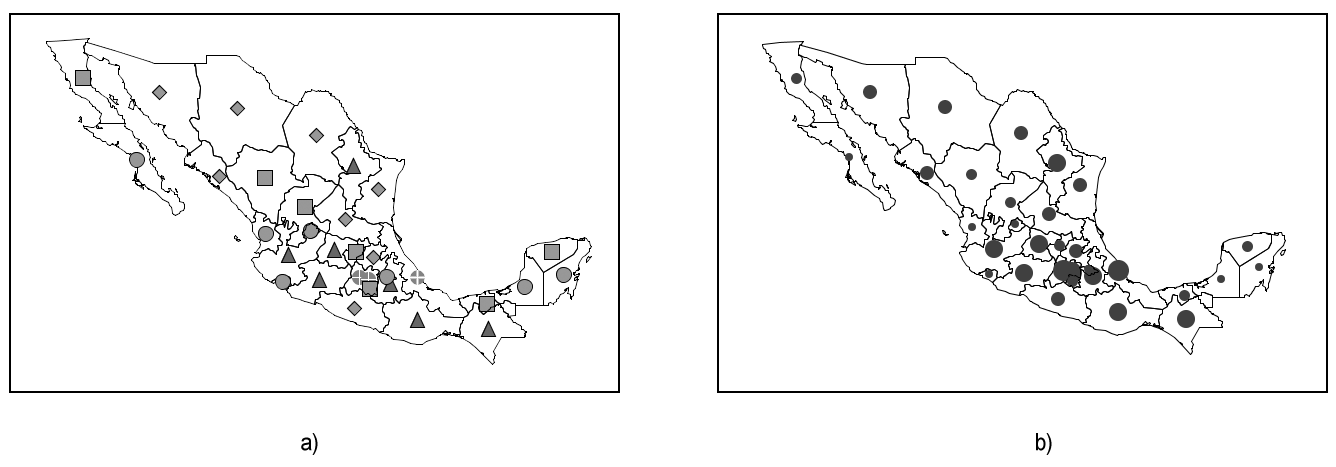
\includegraphics[width=0.95\mycolumnwidth]{Mapas/LeerVer.png}
\caption{\small Comparaci�n entre una representaci�n incorrecta de la informaci�n por no emplear un esquema adecuado al tipo de esta (a) y una representaci�n correcta utilizando un esquema coherente (b).}
\label{Fig:LeerVer} 
\end{figure}

Los mapas de la figura representan en ambos casos la poblaci�n de los distintos estados de M�xico, pero en cada uno de ellos se emplea una forma distinta de simbolizar los valores de poblaci�n. En el primero de ellos (caso a) se ha dividido la poblaci�n en cinco clases, cada una de las cuales se identifica mediante un s�mbolo. Los s�mbolos han sido escogidos de forma arbitraria, y no existe una relaci�n entre ellos. Por su parte, el ejemplo b) tambi�n emplea s�mbolos y presenta igualmente cinco clases, pero en este caso tienen todos las misma forma, y lo que var�a es el tama�o. Se puede establecer una relaci�n entre los s�mbolos, ya que estos pueden ordenarse en funci�n de su tama�o.

Siendo la poblaci�n una variable que tambi�n puede ordenarse, el caso b) es claramente m�s adecuado, ya que nos proporciona la informaci�n visual de forma m�s r�pida e inmediata. No solo responde a la pregunta \emph{�qu� poblaci�n tiene esta provincia?}, sino tambi�n a otras como \emph{�d�nde est� la provincia m�s poblada?} En el caso a) podemos conocer tambi�n la poblaci�n de una provincia y si esta es mayor que la de otra, pero necesitamos para ello acudir a la leyenda, ya que no resulta obvio que el s�mbolo cuadrado indique m�s poblaci�n que el s�mbolo c�rculo. Por su parte, el uso de un �nico s�mbolo y la variable visual tama�o es mucho m�s intuitivo, y nos transmite esa informaci�n sin necesidad de consultar la leyenda del mapa. Este hecho est� directamente relacionado con las propiedades de las variables visuales, que ya estudiamos en el cap�tulo \ref{Conceptos_basicos_visualizacion}.

Como argumenta \cite{Bertin1987Pompidou}, el primer mapa es una mapa que debemos \emph{leer}, mientras que el segundo es un mapa que podemos \emph{ver}. Puesto que un mapa es un elemento visual, es preferible que transmita de forma visual su informaci�n, y un mapa a \emph{leer} supone un desperdicio tanto de tiempo como de informaci�n misma.

As� pues, la selecci�n de una forma de simbolizaci�n adecuada en funci�n de la naturaleza de la informaci�n es clave para lograr un mapa efectivo. En particular, debe emplearse una variable visual que presente la propiedad (nivel de organizaci�n) adecuado. Las propiedades asociativa y selectiva solo son de inter�s para informaci�n cualitativa, mientras que, por ejemplo, el tama�o es la �nica variable visual con la propiedad cuantitativa, y por tanto la �nica adecuada para representar razones.

Las siguientes son algunas ideas b�sicas a este respecto referidas a los distintos tipos antes citados.

\index{Informaci�n!tipos}\index{Informaci�n!alfanum�rica}\index{Informaci�n!num�rica}
\begin{itemize}
	\item Nominal. La informaci�n de tipo nominal se representa adecuadamente utilizando la variable visual forma. Lo que representamos responde principalmente a la pregunta \emph{qu�} en lugar de a la pregunta \emph{cu�nto}, y est� m�s relacionado en cierto modo con la cartograf�a base que con la cartograf�a tem�tica. El uso de s�mbolos, es decir, de la variable visual forma, para elementos puntuales o lineales es una soluci�n muy eficaz y habitual en este caso. Para el caso de representar �reas puede emplearse la variable visual color y emplear distintos tonos, o bien la textura (Figura \ref{Fig:RepresentacionInfoNominal}). Como dijimos en su momento, los tonos no presentan un orden (aunque citamos que pueden hacerlo si existe alguna l�gica en la sucesi�n de estos), pero este no es necesario para este tipo de variables. La �nica propiedad que es de inter�s en este caso es la selectiva.
	
	La informaci�n alfanum�rica se trata a efectos de representaci�n del mismo modo que la de tipo nominal.
	
\begin{figure}[!hbt]
\centering
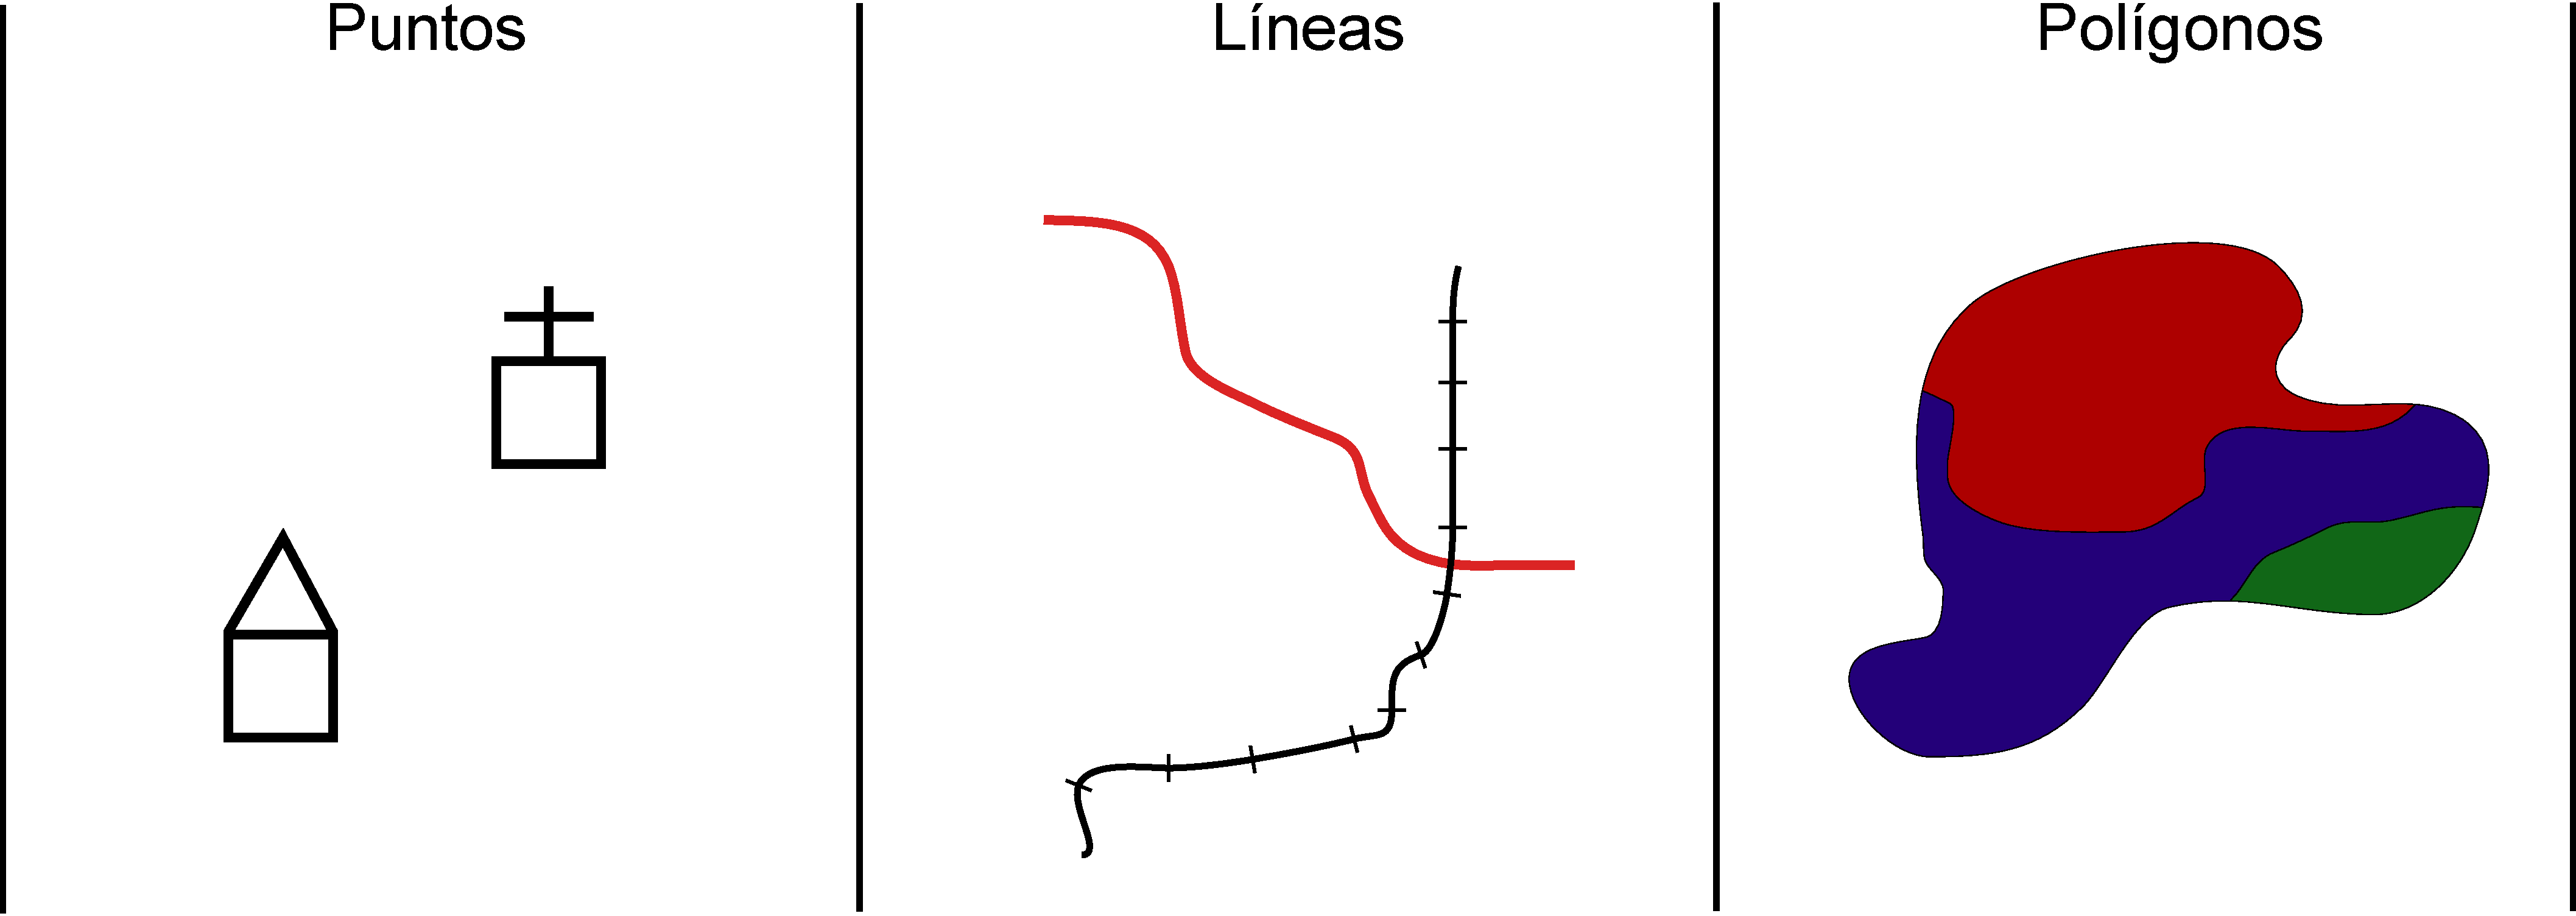
\includegraphics[width=0.90\mycolumnwidth]{Mapas/RepresentacionInfoNominal.pdf}
\caption{\small Representaci�n de la informaci�n nominal para los distintos tipos de elementos geom�tricos.}
\label{Fig:RepresentacionInfoNominal} 
\end{figure}

	\item Ordinal. A diferencia de la informaci�n nominal, en la informaci�n ordinal los valores definen un orden, por lo que la propiedad ordenada es necesaria para poder aplicarla a este caso.
	
	\item Intervalos y razones. Tanto intervalos como razones son tipos de informaci�n con m�s posibilidades que las anteriores, y en las que el n�mero de valores que encontramos a la hora de representar un fen�meno es habitualmente m�s elevado. Frecuentemente, estos valores son de tipo real (no enteros), por lo que es adem�s necesario agruparlos en clases, como veremos en un pr�ximo apartado. Como en el caso anterior, pueden emplearse todas las variables visuales que presenten la propiedad ordenada. No debe olvidarse, no obstante, que la propiedad de mostrar el orden en t�rminos de cantidades o proporciones, que denomin�bamos cuantitativa, es exclusiva del tama�o, siendo este la variable visual m�s adecuada para representar correctamente este tipo de informaci�n y que al visualizar el s�mbolo correspondiente pueda estimarse el valor representado de forma intuitiva.	
\end{itemize}

%Como puede verse, el tipo de elemento geom�trico (punto, l�nea o pol�gono) tiene importancia a la hora de la simbolizaci�n. Esto tiene una obvia relaci�n con los distintos tipos de geometr�as del modelo vectorial, y as� lo veremos cuando apliquemos estas ideas a la visualizaci�n dentro de un SIG en el cap�tulo \ref{Visualizacion_SIG}.

En resumen, podemos condensar este apartado con una r�pida <<receta>> de aplicaci�n general (aunque siempre con excepciones, ya que la representaci�n y simbolizaci�n contiene, no olvidemos, elementos subjetivos), seg�n los siguientes puntos:

\begin{itemize}
	\item Para las variables cualitativas se emplean las variables visuales color, forma y textura, en la medida que sea posible seg�n el tipo de objeto geom�trico a simbolizar.
	\item Para las variables cuantitativas, el valor del color y el tama�o son las m�s adecuadas, siendo esta �ltima la �nica que permite transmitir toda la informaci�n en el caso de variables de tipo razones. El tono de color puede emplearse, pero debe escogerse una gama de tonos que presente alg�n tipo de l�gica que permita establecer un orden.
\end{itemize}

En la figura \ref{Fig:ResumenRepresentacionTiposInformacion} se muestra un cuadro con estas breves ideas.


\begin{figure}[!hbt]
\centering
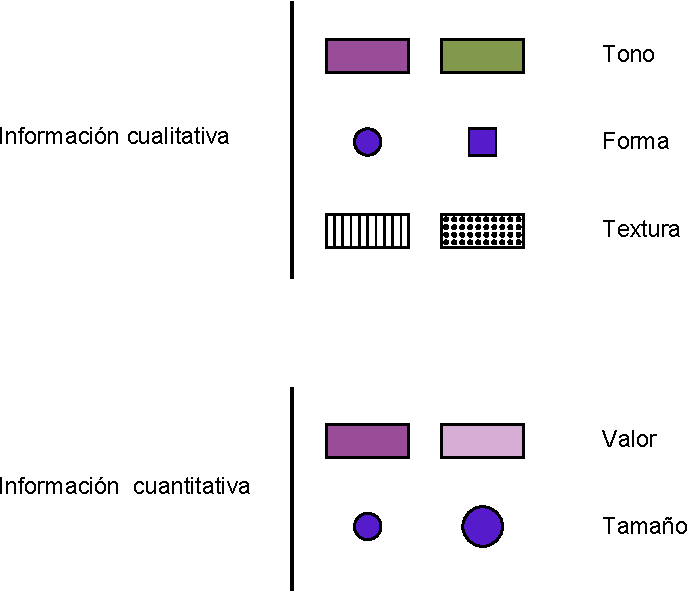
\includegraphics[width=0.6\mycolumnwidth]{Mapas/ResumenRepresentacionTiposInformacion.pdf}
\caption{\small Utilizaci�n de las variables visuales seg�n el tipo de informaci�n.}
\label{Fig:ResumenRepresentacionTiposInformacion} 
\end{figure}

Por �ltimo, es de inter�s se�alar que, aunque los niveles de organizaci�n de las variables visuales expresan a su vez unas posibilidades crecientes (es decir, con una variable como el valor o el tama�o podemos expresar todo lo que el tono puede transmitir, ya que est�n en un nivel superior), ello no implica necesariamente que el uso de una variable de un nivel superior es mejor que otra de uno inferior. Podemos ver esto claramente en la figura \ref{Fig:MalUsoValor}. En ella se ha utilizado la variable valor para representar un mapa con informaci�n cualitativa. Puesto que el valor tiene la propiedad ordenada, esto puede inducir a pensar que existe alg�n orden en la variable representada (tipos de suelo en este caso). Adem�s, y debido a que el valor es disociativo, algunos elementos son m�s llamativos, lo que puede asociar una falsa preponderancia a la clase a la que representan. 

Razonamientos similares se pueden aplicar para el caso particular de capas con variables de tipo verdadero/falso. En estas, deben emplearse colores de similares caracter�sticas, de forma que no exista posibilidad de interpretarlos err�neamente y asociar a alguna de las opciones la idea de ser <<mejor>> que la contraria. Transmitir la informaci�n no es lo �nico que se busca, sino tambi�n hacerlo sin que aparezcan posibles sesgos a la hora de interpretarla.


\begin{figure}[!hbt]
\centering
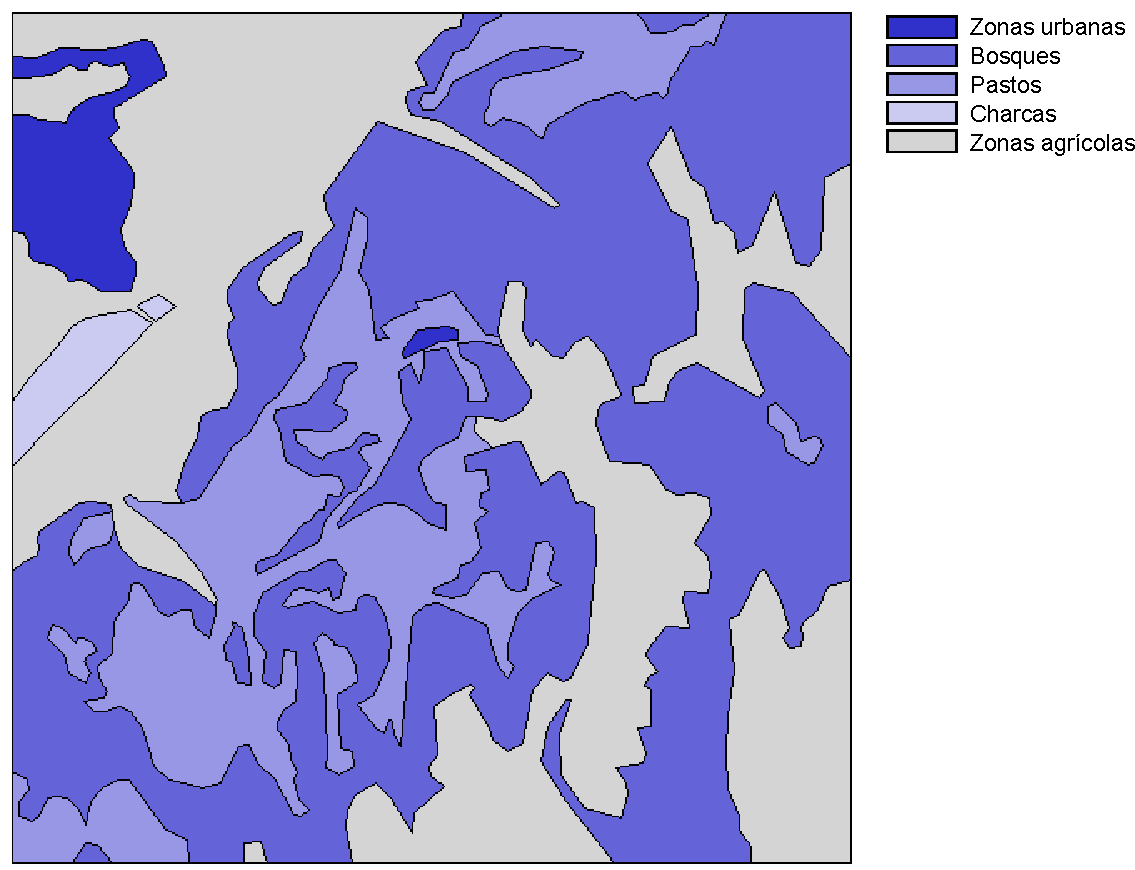
\includegraphics[width=0.6\mycolumnwidth]{Mapas/MalUsoValor.pdf}
\caption{\small Uso incorrecto de la variable visual valor para representar informaci�n cualitativa. Puede transmitirse una falsa sensaci�n de que existe un orden en las clases representadas.}
\label{Fig:MalUsoValor} 
\end{figure}

\subsection{Creaci�n y asignaci�n de clases}\label{CreacionClases}

En el caso de trabajar con informaci�n de tipo intervalos o razones, simbolizar cada uno de los valores de una forma distinta supone la necesidad de emplear un n�mero muy elevado de simbolog�as distintas. Esto puede complicar la interpretaci�n del mapa, especialmente si se lee este junto a su leyenda correspondiente, ya que identificar una simbolog�a concreta en esta es complejo y resulta f�cil equivocarse. Asimismo, con un n�mero elevado de simbolog�as, las diferencias entre estas son peque�as, por lo que tambi�n es complicado separar unas de otras y percibir que dos de ellas son distintas o son la misma. Por esta raz�n, lo habitual es agrupar todo el conjunto de valores disponibles en una serie de categor�as, clasific�ndolos y estableciendo la simbolog�a no en funci�n del valor en s�, sino de la clase a la que pertenece.

La creaci�n de clases para una serie de valores es un problema en el que han de considerarse dos par�metros principales: el n�mero de clases a crear y el criterio a aplicar para establecer los l�mites de cada una.

Respecto al numero de clases, este debe ser lo suficientemente grande como para no resumir en exceso la informaci�n y poder mostrar con un cierto detalle el comportamiento de la variable, pero no demasiado alto para evitar los problemas que aparec�an en el caso de no dividir los valores en clases. El n�mero de clases es tambi�n funci�n de la variable visual utilizada, ya que algunas resultan m�s f�ciles de diferenciar. En general, el m�ximo de clases que se distinguen es del orden de 7 u 8, no siendo recomendable establecer un n�mero mayor, con independencia de qu� variable empleemos. Esto no quiere decir que deban crearse sistem�ticamente 8 clases para cualquier variable y situaci�n, ya que, en funci�n de otros factores, puede resultar de inter�s elegir otro n�mero distinto de clases. De nuevo, no debe perderse de vista la finalidad que va a tener el mapa que estamos dise�ando.

Una vez que hemos decidido el n�mero de clases, debemos definir el rango de valores que cubrir� cada una de ellas. Esto debe llevarse a cabo tratando de maximizar la informaci�n que se transmite y de aprovechar lo mejor posible la variable visual empleada. Por ejemplo, si esta variable es la coordenada valor de un color, debemos tratar que aparezca bien distribuida y que todas las clases tengan un n�mero similar de elementos, para que todos esos valores aparezcan representados en una cantidad similar a lo largo del mapa\footnote{Aunque en un �mbito distinto, si repasas el apartado \ref{ExpansionContraste} dedicado a la expansi�n de contraste en im�genes, encontrar�s una idea similar a esta.}. \index{Expansi�n de contraste}

La conveniencia de usar una u otra definici�n de clases est�, como resulta f�cil deducir, ligada a la propia distribuci�n de los valores de la variable, por lo que estudiar estos es fundamental. Un histograma es una herramienta muy �til para llevar esto a cabo.

De entre los m�todos que se emplean frecuentemente para la creaci�n de clases de forma sistem�tica, cabe destacar los siguientes:

\begin{itemize}	
	\item Intervalos iguales. Simplemente se divide el rango cubierto por los valores en $n$ clases de la misma amplitud, siendo esta igual a $\frac{\mathrm{max} - \mathrm{min}}{n}$. Su principal inconveniente es que puede resultar en clases con muchos elementos y otras pr�cticamente vac�as, en especial si la variable tiene una distribuci�n normal o aparecen elementos con valores at�picos (\emph{outliers}), que desvirt�an el significado del m�ximo y el m�nimo a la hora de calcular la amplitud de cada clase.\index{Outlier}
	\item Intervalos naturales. Basados en la propuesta de \emph{saltos naturales} de Jenks \cite{Jensk1967IYC}, trata de establecer clases lo m�s homog�neas posibles, disminuyendo la varianza de cada clase. De este modo, se obtienen clases que presentan la m�xima variabilidad entre ellas, constituyendo categor�as bien diferenciadas unas de otras. \index{Saltos naturales de Jenks}
	\item Intervalos normales. De especial inter�s para el caso en que la variable presenta una distribuci�n normal. Se toma la media de los valores y se crean los l�mites de cada clase sumando o restando a esta la desviaci�n t�pica o un m�ltiplo de esta.
	\item Intervalos por percentiles. Utilizando percentiles pueden crearse clases de tal modo que todas ellas contengan el mismo n�mero de elementos. Por ejemplo, los \emph{cuartiles} dividir�n el rango de valores en cuatro clases, cada una de ella con igual numero de elementos. En este caso, los l�mites de separaci�n de clases se encontraran en los percentiles del 25, 50 y 75 por cien, respectivamente.
	
	Pueden aplicarse tambi�n los percentiles no sobre la variable que se representa, sino sobre la superficie que ocupan sus distintos valores. Se tiene de este modo los \emph{percentiles de superficie}, que crean $n$ clases, todas ellas representadas en el mapa por una misma superficie.
	\item Intervalos en progresi�n. Pueden emplearse progresiones como la aritm�tica o la geom�trica para crear las clases, en caso de que los valores de la variable a representar muestren un comportamiento seg�n alguna de estas progresiones.
\end{itemize}

Una comparaci�n visual del resultado de aplicar algunos de los m�todos anteriores se muestra en la figura \ref{Fig:TiposIntervalosClases}

\begin{figure}[!hbt]
\centering
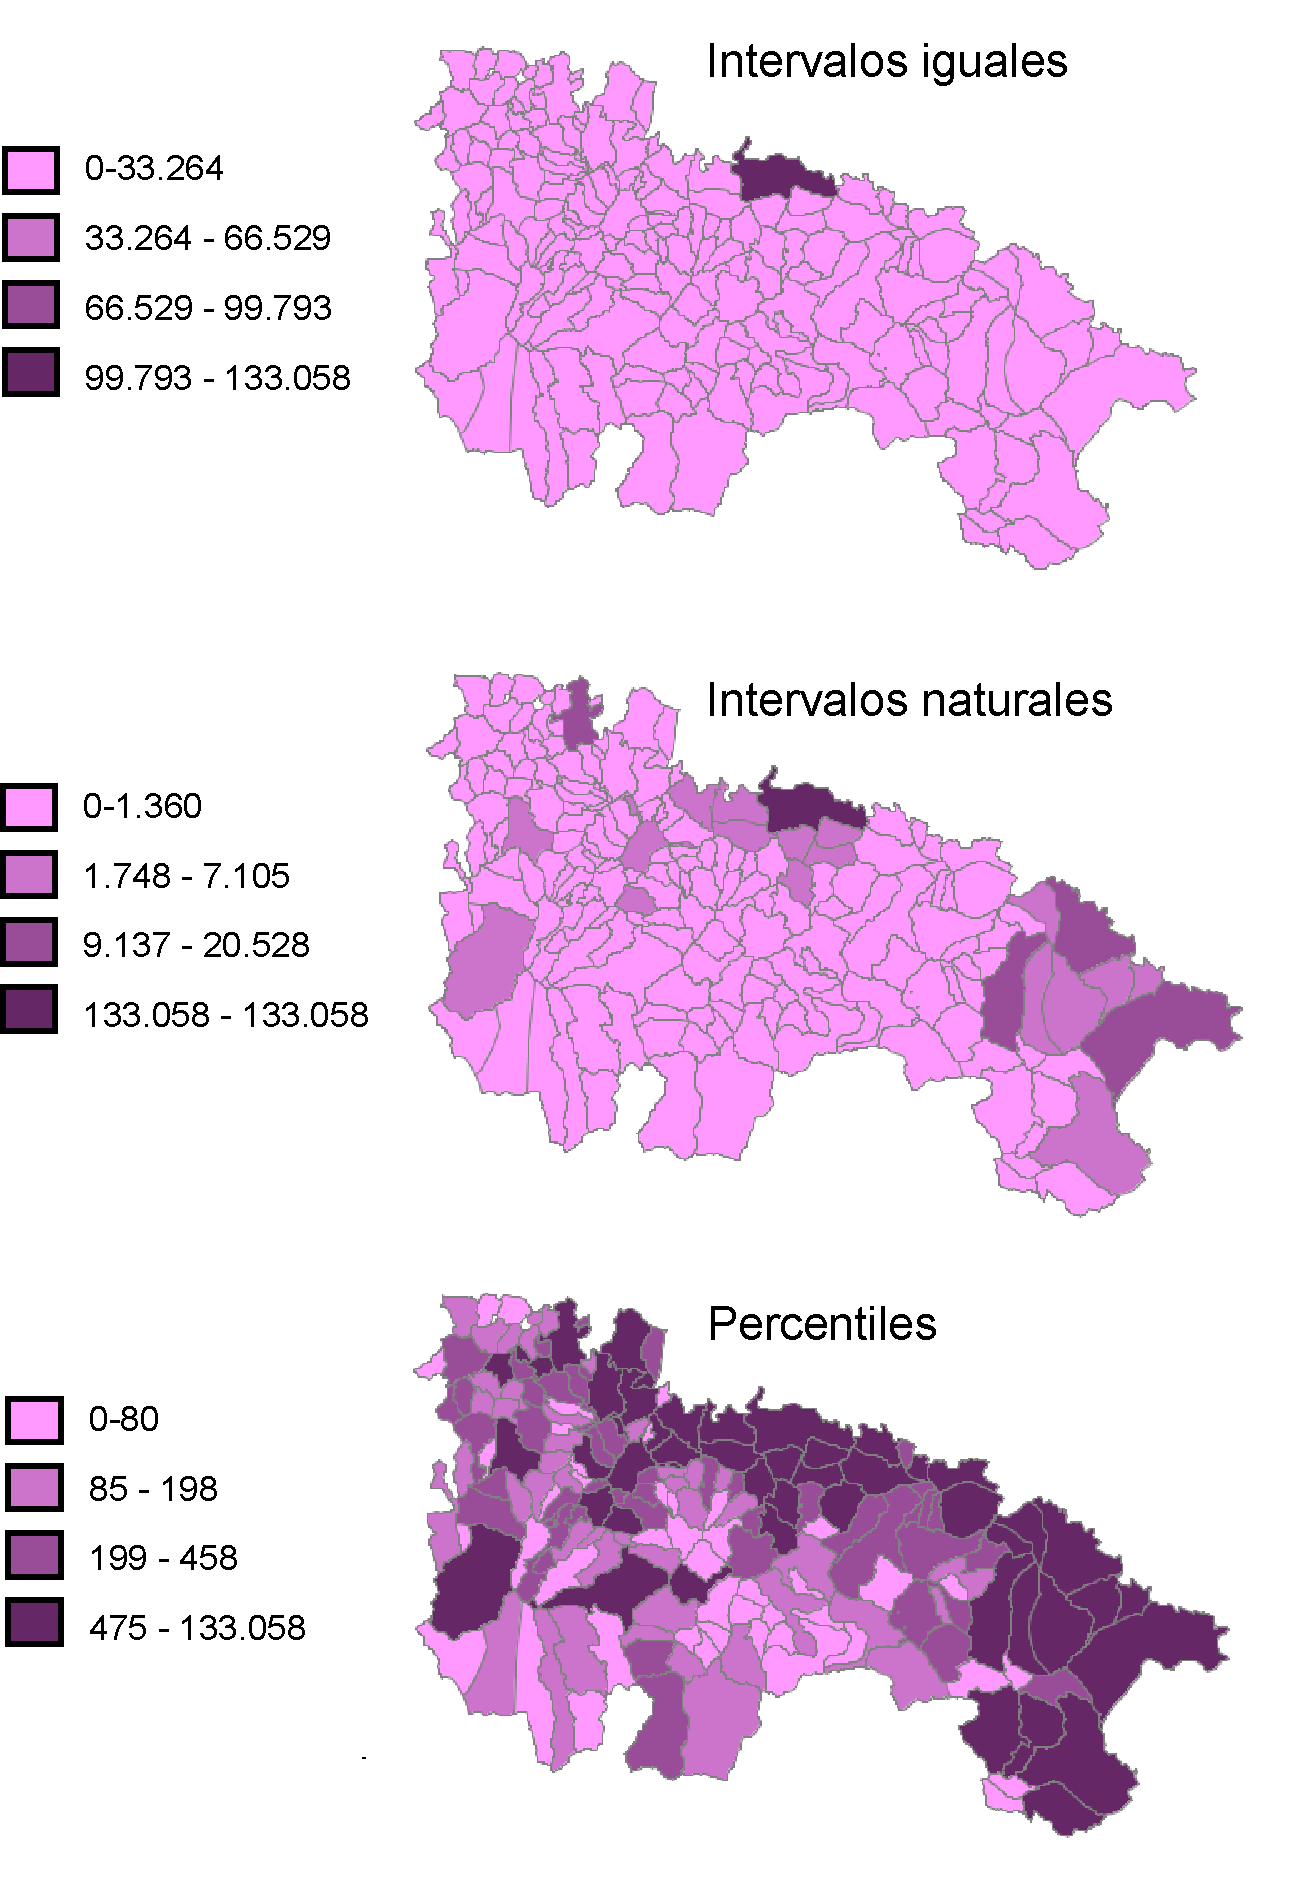
\includegraphics[width=.7\mycolumnwidth]{Mapas/TiposIntervalosClases.pdf}
\caption{\small Comparaci�n entre distintos esquemas para la creaci�n de intervalos de clase.}
\label{Fig:TiposIntervalosClases} 
\end{figure}


Junto a lo anterior, pueden utilizarse transformaciones de los valores previas a su asignaci�n a una clase, para despu�s clasificar el valor transformado. Una transformaci�n logar�tmica es habitual para el caso de valores distribuidos irregularmente, con muchos de ellos en un rango dado y unos pocos en un rango alejado de este. Aplicando un logaritmo (generalmente de base 10), los valores transformados pueden mostrar, por ejemplo, una distribuci�n normal, siendo entonces posible aplicarles una simbolizaci�n mediante intervalos normales. Vimos un ejemplo de esto en la figura \ref{Fig:Transformacion_logaritmica}.

Aunque resulta pr�ctico definir las clases utilizando alguna de las metodolog�as anteriores, pueden igualmente establecerse l�mites de clase arbitrariamente seg�n se considere oportuno en funci�n de la distribuci�n de los valores. Por ejemplo, si existen saltos importantes en esta y quiere rese�arse este hecho, pueden incluirse expl�citamente como l�mites de los intervalos. Asimismo, pueden incorporarse valores particulares que sean de importancia para la variable representada. Esto puede verse claramente en el ejemplo de la figura \ref{Fig:TintasElevacion}

\begin{figure}[!hbt]
\centering
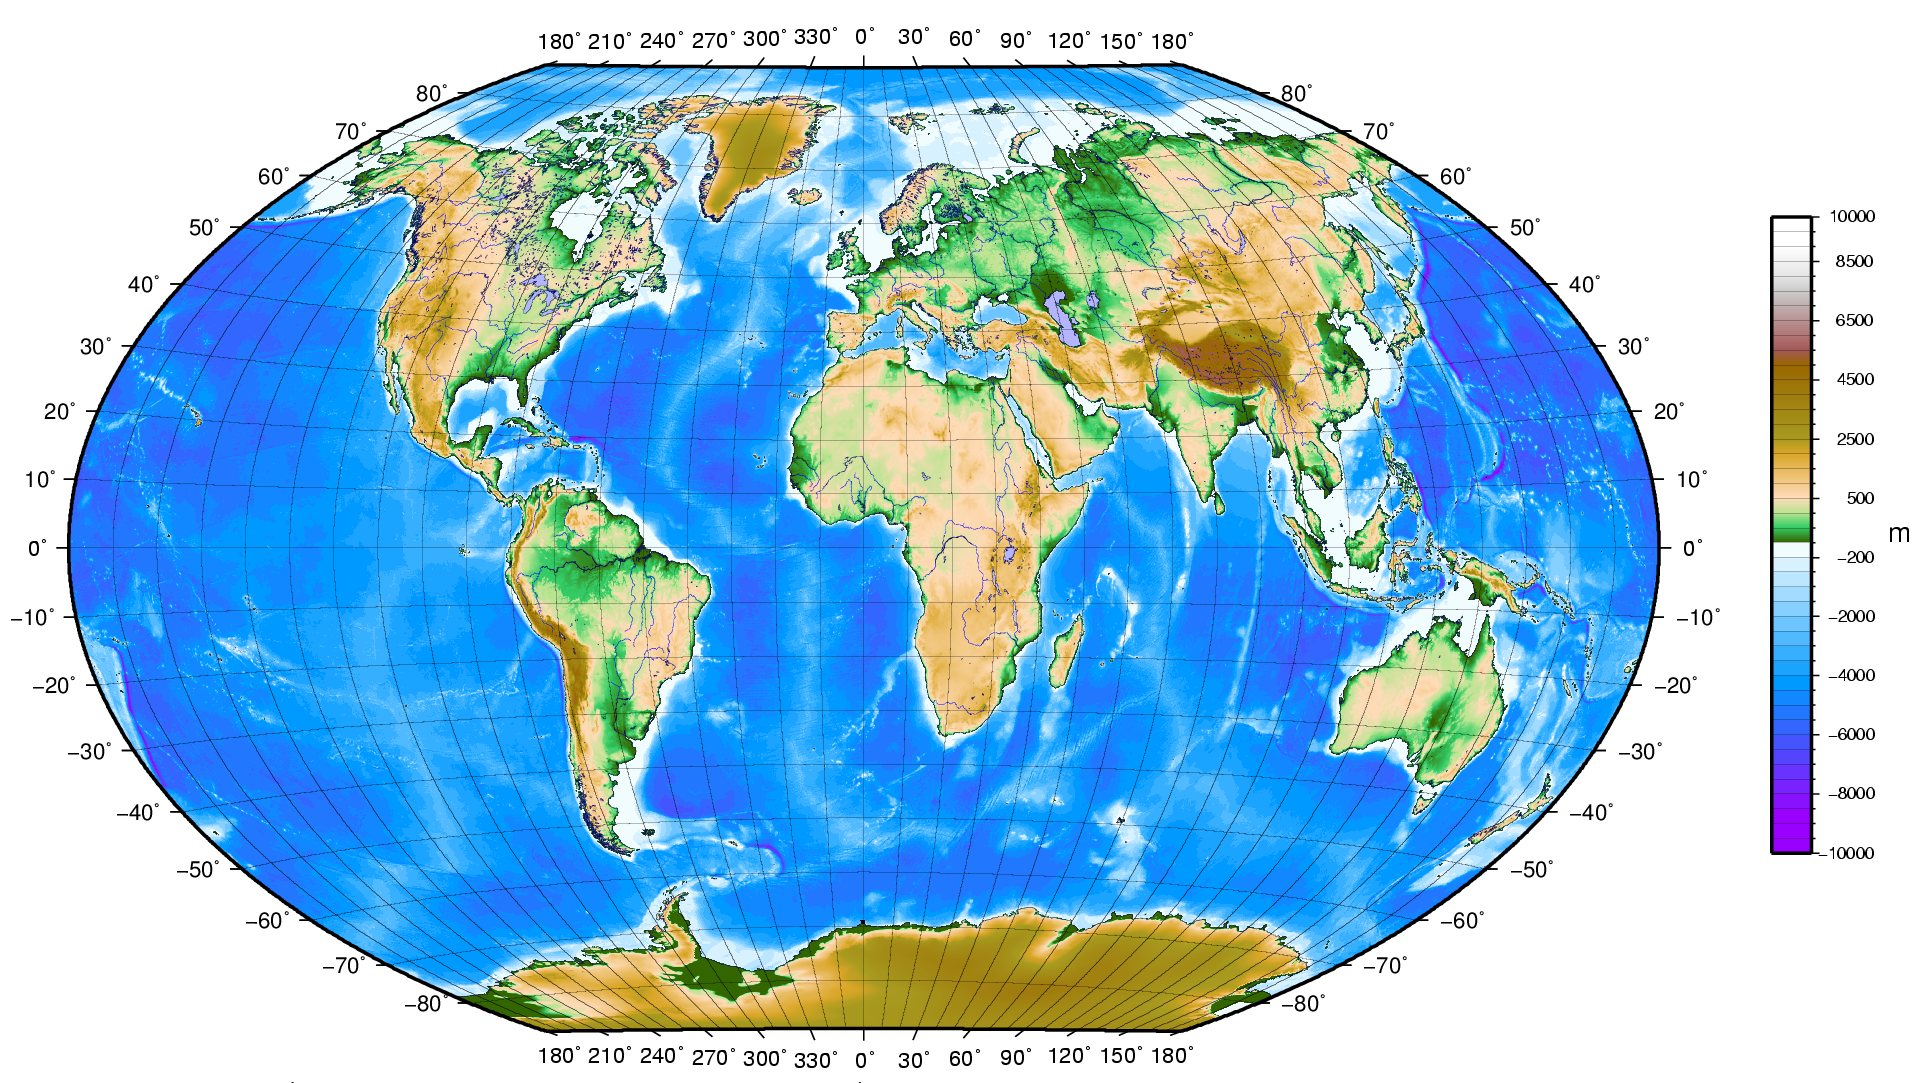
\includegraphics[width=.9\mycolumnwidth]{Mapas/TintasElevacion.png}
\caption{\small Los intervalos pueden incorporar valores de importancia para una determinada variable. En este caso, para la variable elevaci�n resulta particularmente relevante el valor cero, que delimita el comienzo de las clases representadas en azul.}
\label{Fig:TintasElevacion} 
\end{figure}

Para el caso mostrado, en el cual se representa la elevaci�n, es interesante diferenciar los valores positivos (sobre el nivel del mar) de los negativos (zonas por debajo del nivel del mar y, especialmente, batimetr�a del fondo marino). El cero es un valor que puede o no aparecer de modo natural como l�mite de clase al analizar los datos de elevaci�n, pero que se incorpora por su importancia. 

El mapa de la figura presenta adem�s un caso particular por otras razones, ya que utiliza el color como variable ordenada, pese a que dijimos que normalmente no posee tal propiedad. No obstante, este es uno de esos casos en que s� existe un orden f�cil de percibir, ya que los colores escogidos est�n pensados para ser identificados con distintas zonas altitudinales. Las zonas de batimetr�a se representan en tonos de azul, por lo que en ese tramo se est� empleando realmente la componente del color que denomin�bamos valor. Para las restantes, se comienza en el verde (zonas bajas donde crece vegetaci�n que es de ese color), seguido del marr�n (zonas altas sin vegetaci�n) y despu�s el blanco (zonas elevadas que se pueden asociar a nieve). La divisi�n en esos tramos se hace empleando el valor igualmente. Esta asociaci�n de conceptos tan b�sica (y no necesariamente muy real, pero s� conocida y compartida por todo el mundo) permite crear un orden y capacitar a la variable visual color para emplearse a la hora de representar una variable de tipo intervalo como es la elevaci�n.

La presencia del valor cero como punto que define dos mitades (elevaciones sobre el nivel del mar o por debajo de este) hace que los datos de elevaci�n tengan, en lo que a su simbolizaci�n respecta, un esquema de tipo \emph{divergente}. Este tipo de esquemas aparecen cuando la variable presenta alg�n valor cr�tico con un significado particular, dividiendo el conjunto de valores en grupos que pueden considerarse independientes. Es habitual emplear un color de valor bajo (esto es, un color claro) en las cercan�as del punto cr�tico, y aumentar el valor a medida que nos acercamos a los extremos tanto por encima como por debajo de este punto. Cada mitad, a su vez, suele representarse con colores que presentan un fuerte contraste entre s�, para de este modo indicar que cada una de ellas representa una realidad bien distinta de la otra.

Los esquemas no divergentes para variables cualitativas se dice que son de tipo \emph{secuencial}.

Debe rese�arse que, en el caso de establecer las clases en funci�n de los datos, tal y como sucede al aplicar los m�todos que hemos descrito, la simbolizaci�n no ser� adecuada para realizar comparaciones con otros mapas. Un mismo valor puede simbolizarse con colores distintos en sendos mapas, ya que la clase a la que pertenece depende del resto de valores en su conjunto, por lo que no tiene sentido una comparaci�n visual. Por el contrario, si el intervalo se define sin considerar los valores particulares del conjunto representado (como en el mapa de elevaciones anterior), el mismo color en dos mapas s� que implica un mismo rango de valores, con lo que pueden efectuarse comparaciones.

Si quieres experimentar con la definici�n de clases y la asignaci�n de colores a estas, una herramienta de enorme valor es la que encontrar�s en la pagina Web \url{http://www.colorbrewer.org}. �sala no solo para probar ahora todo lo explicado en este cap�tulo, sino tambi�n cuando tengas que crear tus propios mapas. Elegir un adecuando conjunto de colores y clases no es una tarea sencilla, y una herramienta as� puede aportar mucho valor a tus mapas si la empleas correctamente junto a las propias funcionalidades del SIG que est�s utilizando.

\section{Elementos del mapa. Composici�n}

Un mapa no es solo una colecci�n de gr�ficos que representan objetos o valores del mundo real a una escala dada, sino que para ser verdaderamente completo requiere completarse con otra serie de elementos adicionales. Es decir, el mapa en s� no es solo lo que se deriva de la representaci�n de la informaci�n geogr�fica y su simbolizaci�n, sino un conjunto de elementos dispuestos de forma �ptima, entre los cuales, eso s�, resulta de particular relevancia aquel que contiene la informaci�n geogr�fica como tal.

Igual de importante que simbolizar correctamente la informaci�n geogr�fica es situar adecuadamente los distintos elementos del mapa, ya que estos est�n pensados tambi�n, al igual que la propia simbolog�a, para facilitar la interpretaci�n de la informaci�n y hacer esta m�s comprensible.

Los siguientes son los elementos fundamentales que podemos emplear para componer un mapa (Figura \ref{Fig:ElementosMapa}):

\begin{figure}[!hbt]
\centering
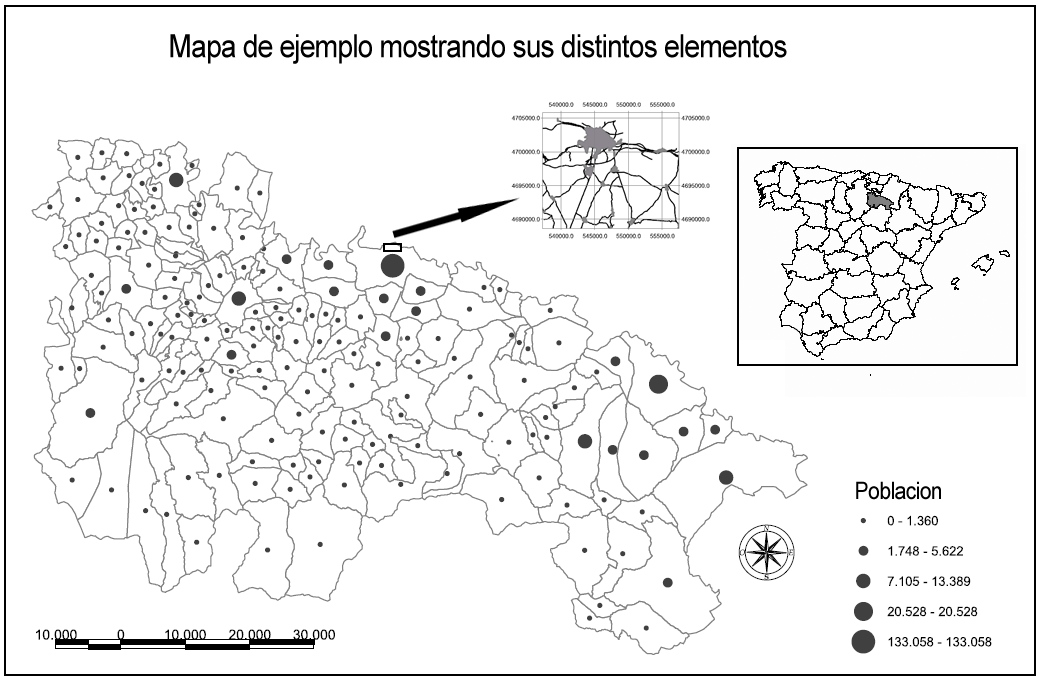
\includegraphics[width=\mycolumnwidth]{Mapas/ElementosMapa.png}
\caption{\small Ejemplo de mapa mostrando sus elementos m�s habituales.}
\label{Fig:ElementosMapa} 
\end{figure}

\begin{itemize}
\item Nombre o t�tulo. Imprescindible para conocer qu� informaci�n muestra el mapa.
	\item Autor. La persona u organismo que ha creado el mapa debe aparecer indicada en alg�n punto de este.
	\item Otra informaci�n sobre el mapa. Por ejemplo, la relativa al sistema de referencia empleado o la fecha de su creaci�n, entre otras.
	\item Canev�s. El canev�s nos indica d�nde dentro de la superficie terrestre se encuentra aquello que el mapa representa, y provee la referencia geogr�fica para sus elementos. Asimismo, complementa a la escala para la estimaci�n visual de distancias y medidas. Es m�s necesario en caso de escalas bajas, aunque se a�ade con independencia de la escala.\index{Canev�s}
	\item Leyenda. Aunque se ha de tratar de utilizar una simbolog�a lo m�s expresiva posible, no toda la informaci�n puede incorporarse en el mapa, y es necesario acompa�arlo de una leyenda. Esta ha de ser tambi�n f�cil de interpretar y lo m�s clara posible. Una leyenda demasiado extensa o de dif�cil comprensi�n probablemente nos indica que la simbolog�a escogida es mejorable.
	
	La leyenda es un elemento dif�cil de crear, aunque los SIG normalmente presentan funcionalidades de creaci�n autom�tica de esta. No obstante, la calidad del resultado suele ser pobre, y es habitual que exista siempre la posibilidad de editarla manualmente con posterioridad para corregir sus deficiencias. Un error com�n es mostrar los valores exactos de los intervalos de clase, una precisi�n muchas veces innecesaria. Por ejemplo, para los mapas de la figura \ref{Fig:TiposIntervalosClases}, que representan la variable poblaci�n, los l�mites de los intervalos no son en algunos casos valores enteros debido a la propia naturaleza del m�todo empleado para crearlos, pero la poblaci�n s� que ha de ser siempre expresada con un valor entero. Expresar el rango de cada clase con un numero amplio de decimales (tal y como las rutinas automatizadas del SIG suelen hacer) no resulta muy adecuado, por lo que deben sustituirse las cifras por las correspondientes redondeadas, sin que ello reste utilidad o exactitud a la leyenda.
	
	La leyenda y el mapa en s� forman un todo, por lo que no deben separarse mediante un cuadro, salvo en el caso en que el mapa cubra todo el �rea del lienzo y no sea f�cil separar visualmente de forma clara ambos elementos.
	\item Norte. Aunque habitualmente se presupone la orientaci�n Norte-Sur, no siempre ha de ocurrir as�, y una aguja apuntando al norte o una rosa de los vientos sirve para aclarar la orientaci�n del mapa. Es de rese�ar que la orientaci�n no ha de ser constante para todos los puntos de un mapa, estando esto en relaci�n con el tipo de sistema de coordenadas y la proyecci�n empleada. Por ejemplo, en el mapa mundial de la figura \ref{Fig:TintasElevacion}, el Norte se sit�a hacia arriba de la hoja solo en el centro. Si nos encontramos en la parte izquierda del mapa la direcci�n del Norte no es la misma. El canev�s, que contiene los paralelos y meridianos, ser� en este caso la referencia fiable en lo que a orientaci�n respecta.
	\item Escala. La escala debe indicarse tanto de forma num�rica como gr�fica, de modo que puedan realizarse c�lculos y estimar visualmente distancias entre puntos dados del mapa.\index{Escala}
	\item Localizador. Un localizador provee un elemento visual para situar el mapa en un contexto geogr�fico m�s amplio, de modo similar al canev�s. Es de especial inter�s en el caso de series de mapas, para establecer la relaci�n entre el presente y los restantes dentro de la misma serie. En este caso, el localizador sirve como mapa �ndice.
	\item Mapas de detalle. Cuando resulta necesario mostrar una cierta zona del mapa con mayor detalle y a una escala mayor, se puede incluir un mapa correspondiente a esa zona como un enclavado dentro del mapa principal. Se debe se�alar asimismo sobre este �ltimo la zona a la que corresponde el mapa de detalle.
\end{itemize}


Aunque en un mapa en sentido cl�sico deben incorporarse todos o la gran mayor�a de los anteriores elementos, cuando trabajamos con representaciones dentro de un SIG la situaci�n es distinta y se puede prescindir de una buena parte de ellos. Por ejemplo, y dado el car�cter menos persistente de la representaci�n en pantalla, a�adir el nombre del autor carece la mayor�a de las veces de sentido. Informaci�n tal como la procedencia de los datos que estamos visualizando resulta de m�s inter�s que el autor del mapa, pero lo correcto es consultar esta en los propios datos, que deber�an contenerla de alg�n modo (veremos m�s sobre esto en el cap�tulo \ref{Metadatos}).

La escala es adecuado mostrarla de forma num�rica, pero no en su versi�n gr�fica, ya que dentro de un SIG encontramos herramientas que nos permiten medir con total precisi�n distancias y �reas, y una escala gr�fica carece de utilidad en este contexto. Por su parte, el localizador es mejor que el canev�s para definir el contexto, ya que muchas aplicaciones SIG incorporan incluso un localizador interactivo sobre el que puede operarse para cambiar el encuadre del mapa.

En lo que respecta a la forma de disponer los elementos sobre el lienzo que un mapa conforma, la premisa fundamental es maximizar la claridad y aprovechar de la mejor forma posible el espacio disponible. La figura \ref{Fig:AprovechamientoEspacioMapa} muestra un claro ejemplo de c�mo un adecuado uso del espacio en el mapa, evitando que existan zonas en blanco que no comunican ninguna informaci�n, mejora notablemente la calidad del mapa.

\begin{figure}[!hbt]
\centering
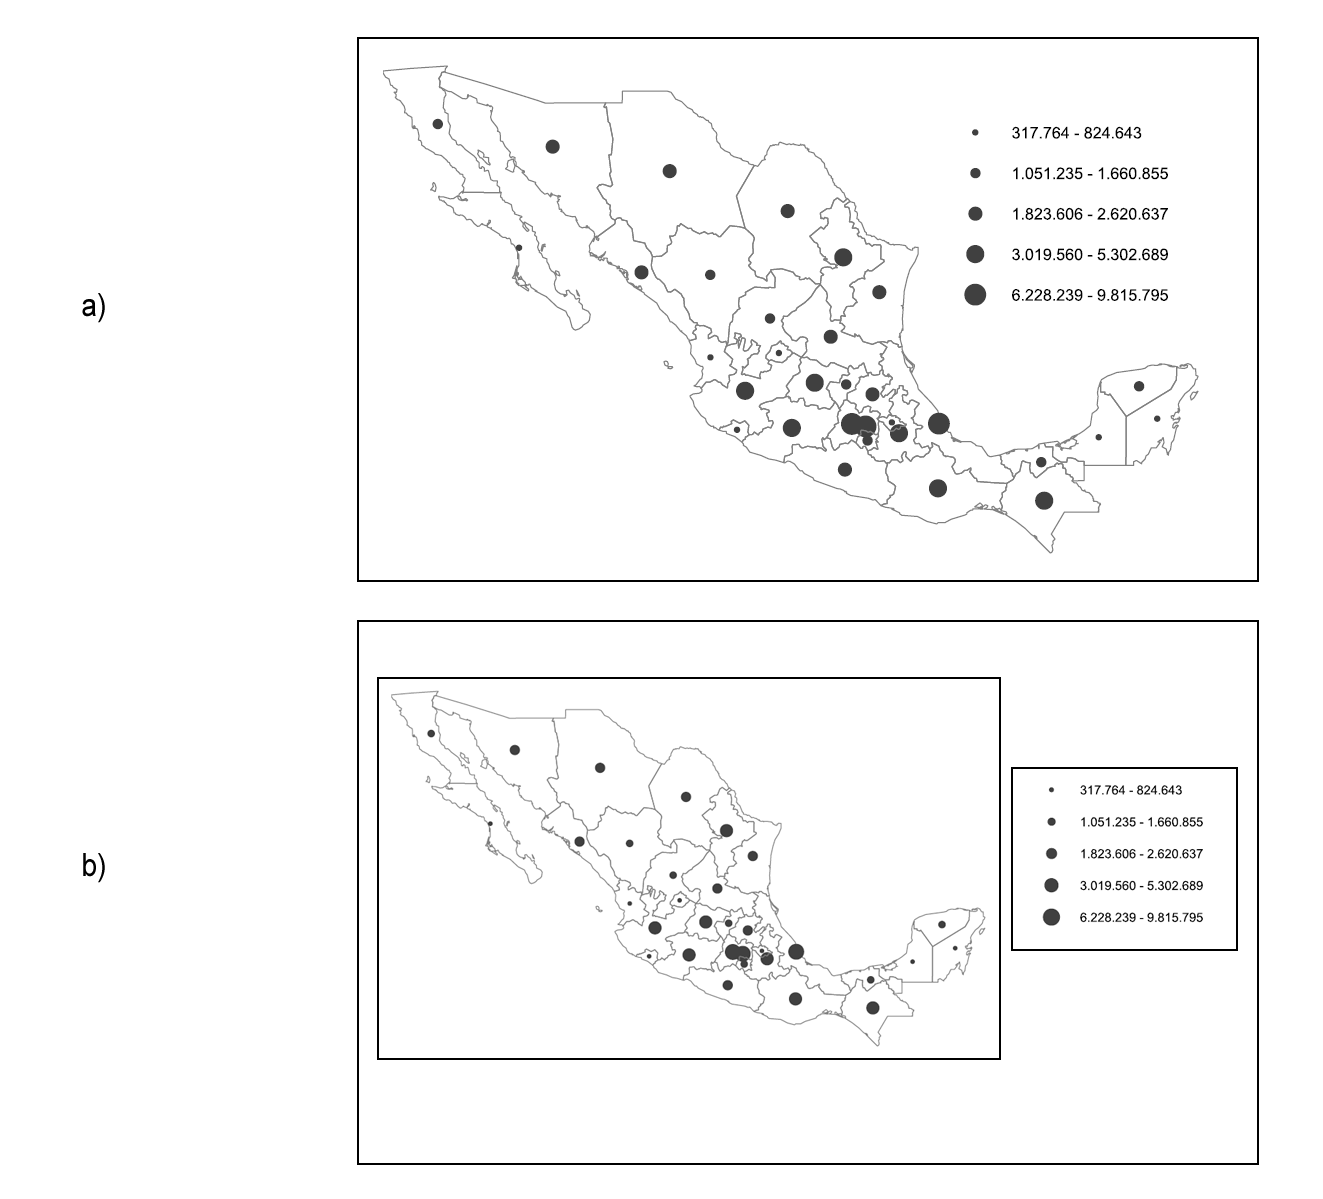
\includegraphics[width=.85\mycolumnwidth]{Mapas/AprovechamientoEspacioMapa.png}
\caption{\small Ejemplo de un aprovechamiento �ptimo del espacio de un mapa (a) y un aprovechamiento incorrecto de este (b).}
\label{Fig:AprovechamientoEspacioMapa} 
\end{figure}

Asimismo, es importante que el dise�o del mapa recalque su prop�sito, haciendo �nfasis en los aspectos m�s relevantes para cumplir este.

Aunque el objetivo principal del dise�o cartogr�fico es crear un mapa �til y no un mapa bonito, no cabe duda que una cierta preocupaci�n por el aspecto est�tico es recomendable, ya que tambi�n contribuir� a una mejor interpretaci�n de la informaci�n del mapa. Este es un aspecto subjetivo y con una componente principalmente art�stica, aunque tambi�n pueden aportarse algunos elementos metodol�gicos de car�cter m�s sistem�tico. Uno de ellos utilizado frecuentemente es el empleo de la proporci�n �urea para dimensionar los elementos del mapa. Comenzando por las dimensiones del propio lienzo, puede aplicarse a las de los restantes componentes, tales como la leyenda en caso de estar situada en un cuadro aparte, o el cuadro que contiene el nombre del mapa y otra informaci�n adicional.\index{Proporci�n �urea}

Los conceptos que deben manejarse a la hora de elegir las caracter�sticas de los elementos del mapa y su emplazamiento derivan de la percepci�n visual, disciplina que ya vimos en el cap�tulo anterior. A continuaci�n tienes algunas ideas adicionales sobre percepci�n visual que deben aplicarse a la composici�n de mapas. Si deseas ampliar estos conceptos, la referencia fundamental sobre percepci�n visual desde el punto de vista del arte es \cite{Arnheim1986Paidos}.\index{Percepci�n visual}

\begin{itemize}
\item El documento cartogr�fico tiene dos centros. Un centro geom�trico y uno �ptico. Este �ltimo se sit�a por encima del geom�trico, aproximadamente a un 5\% de la altura total del documento. Los elementos del mapa se deben disponer alrededor del centro �ptico.
	\item Los elementos en la parte superior del mapa tienen una mayor importancia, as� como los situados en la parte izquierda. Es en estas zonas donde deben situarse los elementos m�s importantes sobre los que se quiera centrar la atenci�n.
	\item La atenci�n del lector del mapa va desde la esquina superior izquierda hasta la inferior derecha, pasando por el centro �ptico. Los elementos importantes deben situarse en esta l�nea, para que su posici�n se corresponda con los movimientos naturales de la vista.
	\item Debe tratarse de crear un mapa sea visualmente equilibrado. El equilibrio visual es el resultado del peso que cada elemento tiene y su posici�n, as� como su orientaci�n. Estos pesos deben repartirse adecuadamente por todo el lienzo del mapa. El peso de un elemento depende de m�ltiples factores, entre ellos los siguientes: \index{Centro!�ptico del mapa}\index{Equilibrio visual}
	
\begin{itemize}
	\item Posici�n. Los elementos tiene m�s peso en la derecha que en la izquierda, y m�s en la parte superior que en la inferior. El peso aumenta al aumentar la distancia al centro del documento.
	\item Tama�o. Mayor tama�o implica m�s peso.
	\item Color. Los colores brillantes tienen m�s peso que los oscuros. El tono rojo tiene m�s peso que el azul.
	\item Aislamiento. Los elementos aislados tienen m�s peso que aquellos rodeados por otros.
	\item Forma. Las formas regulares tienen m�s peso que las irregulares. Cuanto m�s compacta sea la forma, tambi�n tendr� m�s peso.
	\item Direcci�n. Algunos elementos pueden tener una direcci�n que <<dirija>> la atenci�n hacia otros, concedi�ndoles peso (por ejemplo, una flecha que se�ale a un elemento, haciendo que llame m�s la atenci�n),
\end{itemize}

\end{itemize}

Las ideas acerca de la composici�n y el equilibrio del mapa se han de aplicar a todo el documento cartogr�fico (es decir, al que contiene todos los elementos citados anteriormente), as� como a la parte de este que representa la informaci�n geogr�fica. Es importante seleccionar adecuadamente el �rea geogr�fica cubierta para que la informaci�n relevante que se muestra acerca de esta conforme un conjunto equilibrado y siga a su vez las indicaciones mencionadas. 

Recordar, por �ltimo, que la composici�n del mapa implica una organizaci�n horizontal (plana) de sus elementos, pero existe asimismo una organizaci�n vertical. Esta viene definida por la jerarqu�a existente, sobre la cual ya se comentaron algunas ideas en el apartado \ref{AyudasPercepcion}. Estas ideas deben aplicarse igualmente en la composici�n del mapa, para conjuntamente lograr un documento equilibrado en el que quede claro qu� elementos son los de mayor importancia y pueda accederse con facilidad a la informaci�n que contienen.

\section{Tipos de mapas tem�ticos}

Los mapas tem�ticos representan la mayor parte de los creados en un SIG, por lo que resulta necesario ver en detalle las formas en las que pueden presentarse. Existen diversas alternativas en funci�n del tipo de elemento que se pretenda simbolizar o las caracter�sticas de la variable tratada, y la elecci�n de una u otra supondr� una diferencia importante en el mapa obtenido y en su uso posterior. En un mismo mapa pueden combinarse varias de estas formas, especialmente si se pretende representar m�s de una variable, en cuyo caso la combinaci�n debe buscar la m�xima claridad en la representaci�n de todas ellas.

En este apartado detallaremos los siguientes tipos de mapas tem�ticos: mapas de coropletas, mapas de isol�neas, mapas de densidad de puntos y mapas de s�mbolos proporcionales. Todos ellos se utilizan para la representaci�n de variables cuantitativas.


\subsection{Mapas de s�mbolos proporcionales}\label{MapasSimbolosGraduados}

Un mapa de s�mbolos proporcionales representa variables cuantitativas a trav�s de s�mbolos cuyo tama�o esta en relaci�n con el valor a representar de dicha variable. Es decir, emplea la variable visual tama�o, que como ya hemos visto es la �nica que presenta la propiedad cuantitativa. La forma de los distintos s�mbolos es siempre la misma, y por simplicidad lo m�s frecuente es utilizar como s�mbolo base el c�rculo, aunque puede utilizarse cualquier otro, e incluso s�mbolos de tipo lineal (barras).\index{Mapa!de s�mbolos proporcionales}

Puesto que el tama�o es el elemento que diferencia a los distintos s�mbolos y el que transmite la informaci�n cuantitativa, su elecci�n es crucial para la creaci�n de un buen mapa de este tipo. La elecci�n de un tama�o implica elegir uno m�nimo y uno m�ximo, correspondientes a los valores m�nimo y m�ximo de la variable en el mapa. Entre estos se situar�n los distintos tama�os correspondientes al resto de posible valores que toma la variable.

Existe, claramente, una relaci�n entre el tama�o m�ximo y el m�nimo, ya que se define una relaci�n de escalado de los distintos valores. Este escalado es distinto para s�mbolos lineales que para s�mbolos de �rea, ya que la percepci�n de la relaci�n entre ellos es distinto seg�n el tipo de s�mbolo empleado. En ambos casos, el escalado debe ser coherente con el valor que se representa, de tal modo que si el usuario del mapa percibe que el tama�o de un s�mbolo es el doble que el de otro, los valores de ambos s�mbolos est�n igualmente en esa proporci�n.

Para conseguir esto se ha de seleccionar el tama�o asociado al valor de uno de los extremos. Esto se har� con un criterio puramente gr�fico, de tal modo que, si por ejemplo establecemos el tama�o m�ximo, este no sea excesivo y a la hora de representar el s�mbolo correspondiente en el mapa ocupe demasiado espacio y existan solapes. Debe evitarse asimismo que el tama�o m�nimo sea demasiado peque�o y no se aprecie el s�mbolo con claridad. Una vez hecho esto, se establece una relaci�n lineal, de tal forma que podemos calcular el tama�o correspondiente a todo valor. Si un valor de 100 se corresponde con una barra de una altura de 10mm, entonces un valor de 200 se representara mediante una barra de 20mm, y as� sucesivamente.

Para el caso de s�mbolos superficiales, no obstante, el escalado no debe hacerse en funci�n de un par�metro lineal (por ejemplo, el radio en el caso de emplear c�rculos), sino respecto a la propia superficie. Es decir, si un valor de 100 se representa con un circulo de radio $r$, el valor 200 no se representar� mediante un c�rculo de radio $r'=2r$, sino con una de tal radio que la superficie sea el doble del primero. En este caso, el radio buscado ser�a $r' = \sqrt{2}r$.

El escalado de s�mbolos se puede dar de forma continua, de tal modo que cada valor se representa con un s�mbolo de un tama�o calculado seg�n la idea anterior, empleando el valor exacto para el escalado. No obstante, la capacidad de diferenciar visualmente tama�os distintos e interpretar la relaci�n entre ellos es limitada, por lo que suele resultar m�s conveniente efectuar un escalado discreto. Es decir, crear clases y asignar a un valor no un s�mbolo del tama�o exacto que le corresponder�a, sino el asignado al valor que define a la clase, habitualmente el centro de esta.


Tanto las barras como los c�rculos pueden sectorizarse, mostrando una divisi�n en subclases del valor total que representan. Para el caso de la poblaci�n, podr�an mostrarse las proporciones que corresponden a hombres y mujeres. Este tipo de representaciones, no obstante, son a veces dif�ciles de interpretar en su conjunto, por lo que resulta m�s adecuado crear varios mapas que muestren esa misma informaci�n por separado, en lugar de conjuntamente en uno �nico.

Aunque la variable visual tama�o presenta la propiedad cuantitativa, la percepci�n de la relaci�n de tama�o no es perfecta y existe una cierta imprecisi�n. Esta se debe a muchos factores, como por ejemplo el hecho de que los s�mbolos situados alrededor de uno dado pueden afectar a la percepci�n de su tama�o. Por esta raz�n, es importante para facilitar la correcta interpretaci�n de un mapa de s�mbolos graduados el mostrar en la leyenda la relaci�n entre los distintos tama�os de los s�mbolos y sus valores. Para el caso habitual de emplear c�rculos, esto puede llevarse a cabo mediante elementos gr�ficos como los mostrados en la figura \ref{Fig:EjemplosLeyendaSimbolosProporcionales}

\begin{figure}[!hbt]
\centering
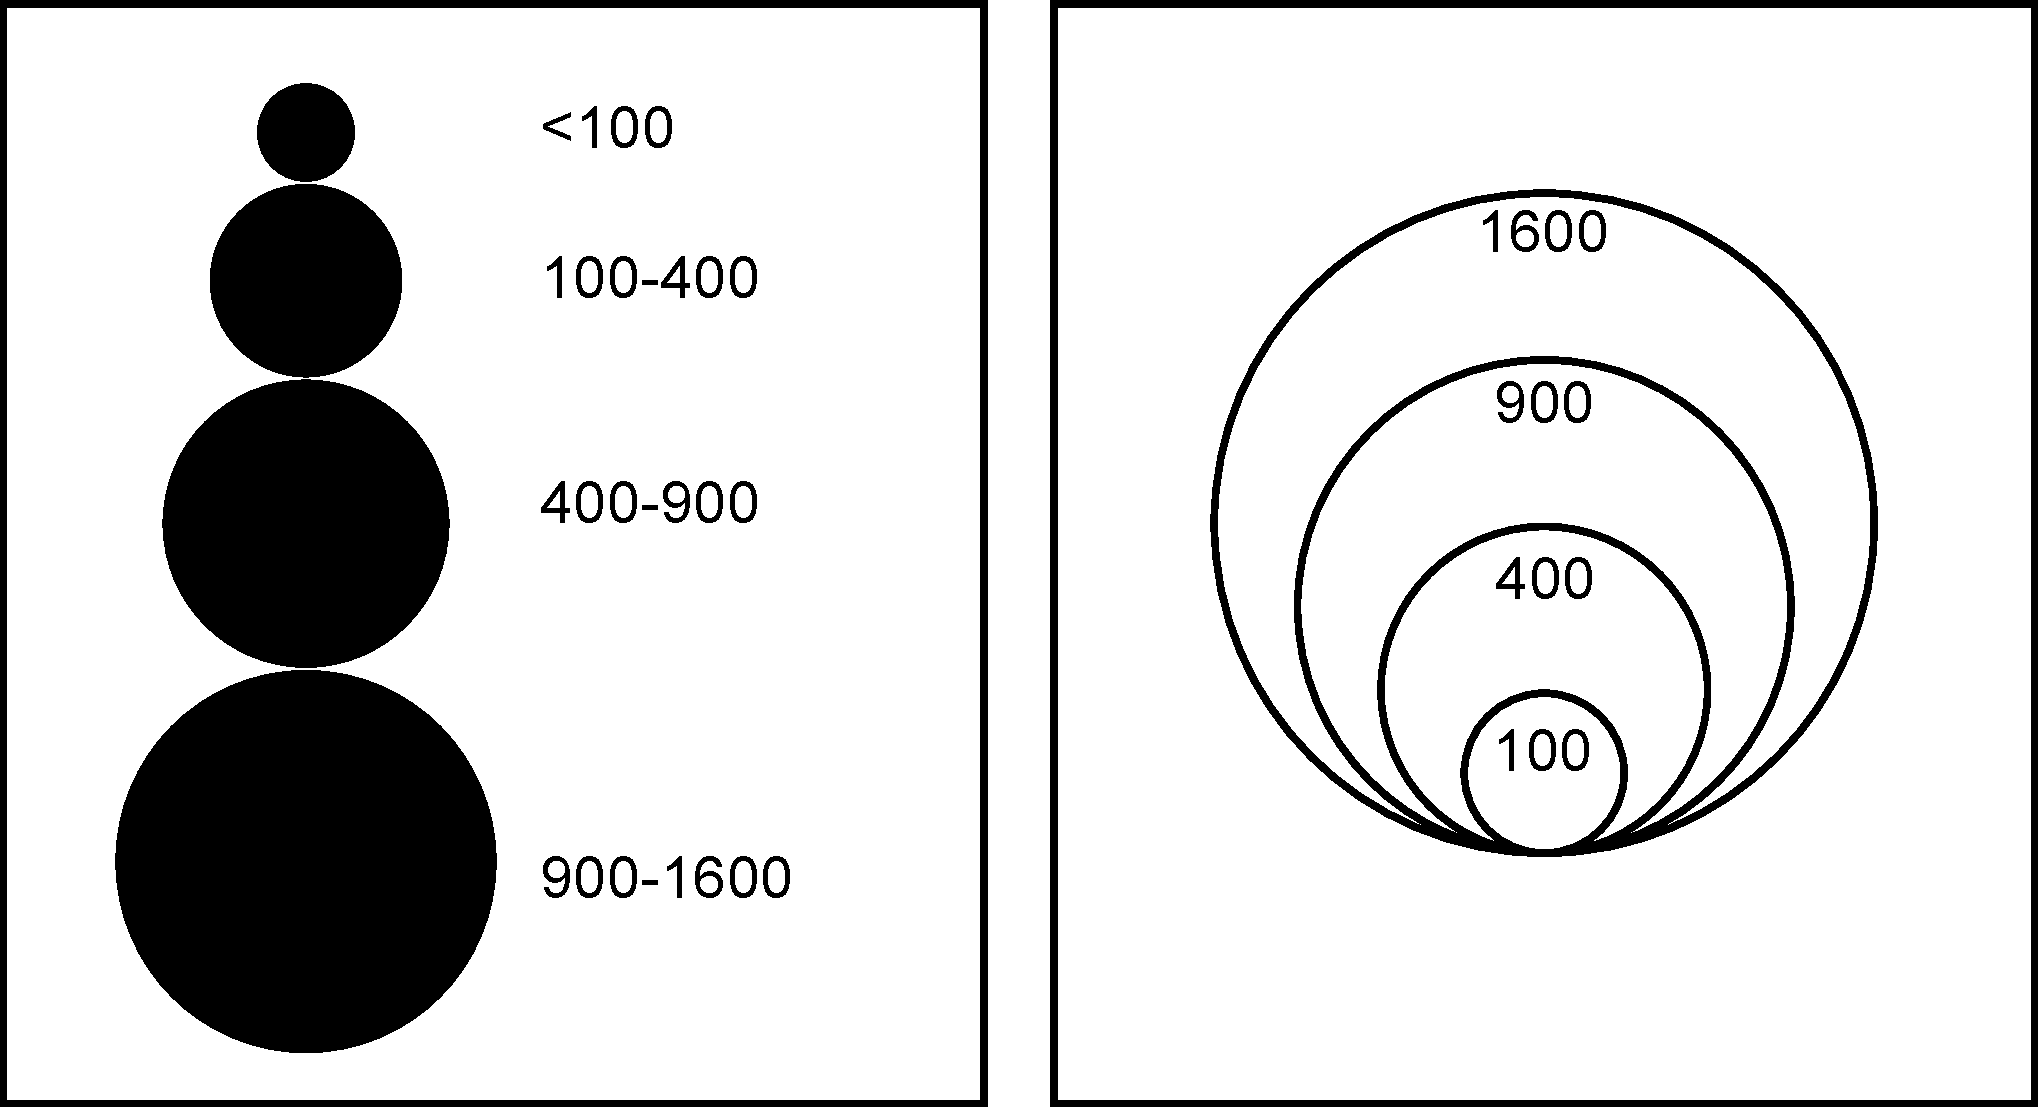
\includegraphics[width=.5\mycolumnwidth]{Mapas/EjemplosLeyendaSimbolosProporcionales.pdf}
\caption{\small Dos ejemplos de leyendas para un mapa de s�mbolos proporcionales.}
\label{Fig:EjemplosLeyendaSimbolosProporcionales} 
\end{figure}

El uso de un escalado lineal en el que se conserve la propiedad cuantitativa resulta en ocasiones inapropiado debido a la distribuci�n de los valores. Por ejemplo, para representar el mapa de la figura \ref{Fig:TiposIntervalosClases}, este esquema no es adecuado, ya que una de las zonas presenta un valor de la variable muy superior a la del resto (puede verse esto claramente en la representaci�n por intervalos iguales), lo cual requerir�a el uso de un s�mbolo desproporcionadamente grande. Si se usan clases iguales, la mayor�a de los valores entrar�an en una de ellas, por lo que no se transmitir�a bien la distribuci�n de estos. En este caso, se debe emplear un esquema de clases distinto, aunque as� la proporci�n de tama�os no permita visualmente estimar las cantidades. Es decir, los tama�os de los s�mbolos nos indican que hay m�s cantidad en una zona que en otra, pero no podemos solo con ellos saber \emph{cu�nto} m�s hay.  Los mapas elaborados de esta forma se conocen como mapa de \emph{s�mbolos graduados}. En estos mapas, la importancia de la leyenda es a�n mayor si cabe, ya que es la encargada de explicar el significado de cada tama�o, y sin ella la informaci�n de la que disponemos es mucho menor.\index{Mapa!de s�mbolos graduados}

El mapa de la figura \ref{Fig:ElementosMapa}, que mostramos al presentar los distintos elementos del mapa, es un ejemplo mapa de s�mbolos graduados.

\subsection{Mapas de puntos}\index{Mapa!de puntos}

Los mapas de puntos se emplean especialmente para la representaci�n de variables que representen alg�n tipo de cantidad, tales como la poblaci�n, el gasto medio por persona o la producci�n de un determinado cultivo. Estas cantidades se representan mediante la repetici�n de puntos, en numero proporcional a su magnitud. Cada uno de esos puntos representa un valor unitario, y el conjunto de ellos sobre la zona en cuesti�n suma la cantidad total a representar. Los puntos tienen todos la misma forma y tama�o, a diferencia de lo que vimos en el caso de los s�mbolos proporcionales.

Los mapas de puntos transmiten de forma muy eficaz los valores que representan, obteni�ndose este por el mero recuento, aunque visualmente permiten una estimaci�n inmediata y pueden compararse entre las distintas zonas del mapa. Por esta raz�n, son especialmente adecuados para variables discretas m�s que para continuas, aunque tambi�n pueden emplearse para estas �ltimas.

Aunque podr�an crearse con cualquier otro s�mbolo, ya que es la repetici�n de este la que transmite la informaci�n, lo m�s habitual es el empleo de puntos, de ah� el nombre gen�rico que se les da.

Tres son los aspectos que deben tenerse en cuenta a la hora de elaborar un mapa de puntos: el valor de cada punto (es decir, cu�ntas unidades de la variable representa cada punto), su tama�o y su posici�n.

Si los valores de la variable que se manejan son bajos, se puede establecer como valor del punto la unidad. Es decir, un punto representa sobre el mapa un habitante en el caso de un mapa de poblaci�n. No obstante, con valores altos (como en el caso de la poblaci�n) esto da lugar a un n�mero demasiado elevado de puntos que saturan el espacio del mapa y no transmiten adecuadamente la informaci�n. Por ello, cada punto debe representar un n�mero mayor de elementos de la variable representada, de tal modo que no aparezcan en demas�a en el mapa, solap�ndose unos con otros. Si el valor escogido es demasiado alto, aparecer�n pocos puntos en el mapa, y este puede quedar poco expresivo y no transmitir la distribuci�n de la variable. Debe, por tanto, escogerse un valor adecuado que equilibre la presentaci�n de los puntos sobre el mapa. Este valor se representar� en la leyenda para su interpretaci�n, habitualmente en forma de texto, escribiendo por ejemplo, que <<un punto equivale a 1000 habitantes>>.

La elecci�n del tama�o del punto debe garantizar la buena visibilidad de este, al tiempo que no debe ser excesivamente grande para que no ocupe demasiado espacio y dificulte la visi�n de otros. Obviamente, el tama�o �ptimo est� en relaci�n con el valor unitario escogido, y ambos par�metros deben establecerse conjuntamente para lograr la combinaci�n m�s adecuada.

Por �ltimo, la posici�n del punto es de gran importancia para transmitir la informaci�n correcta y no dar lugar ambig�edades o incorporar errores conceptuales. Si no disponemos de informaci�n adicional y solo tenemos el valor correspondiente a una zona dada, los puntos se han de disponer de forma regular ocupando toda la superficie de la zona. Si, por el contrario, sabemos algo m�s acerca de la distribuci�n de la variable, debemos emplear esa informaci�n para emplazarlos de forma m�s realista. Si, por ejemplo, la zona corresponde a una provincia y sabemos la localizaci�n de la principal ciudad dentro de ella, es m�s l�gico situar m�s puntos cerca del emplazamiento de esa ciudad que en otras partes de la provincia, ya que una mayor parte de la poblaci�n estar� all�.

Otro aspecto a considerar es el significado de la variable que se representa y la posibilidad o no de que aparezca en las distintas localizaciones de los puntos. Si la variable es, por ejemplo, el numero de ejemplares avistados de un determinado ave acu�tica, situar los puntos sobre zonas urbanas o de bosque no tiene sentido, ya que dan a entender que ah� hay presencia de esa especie (tantos ejemplares como los puntos en cuesti�n indiquen), algo que es falso.

En los dos casos anteriores va a resultar necesario <<mover>> los puntos a su localizaci�n m�s correcta, algo que, habitualmente, no resulta posible con los mecanismos automatizados de que dispone un SIG. El chequeo del mapa creado resulta, por tanto, imprescindible para comprobar que existen puntos en posiciones err�neas. El uso de herramientas externas tales como programas de dise�o gr�fico, seg�n vimos en el cap�tulo \ref{Introduccion_visualizacion}, es una soluci�n para retocar los mapas creados y obtener una distribuci�n de los puntos m�s correcta.

La imagen \ref{Fig:MapaPuntos} muestra un ejemplo de un mapa de puntos.


\begin{figure}[!hbt]
\centering
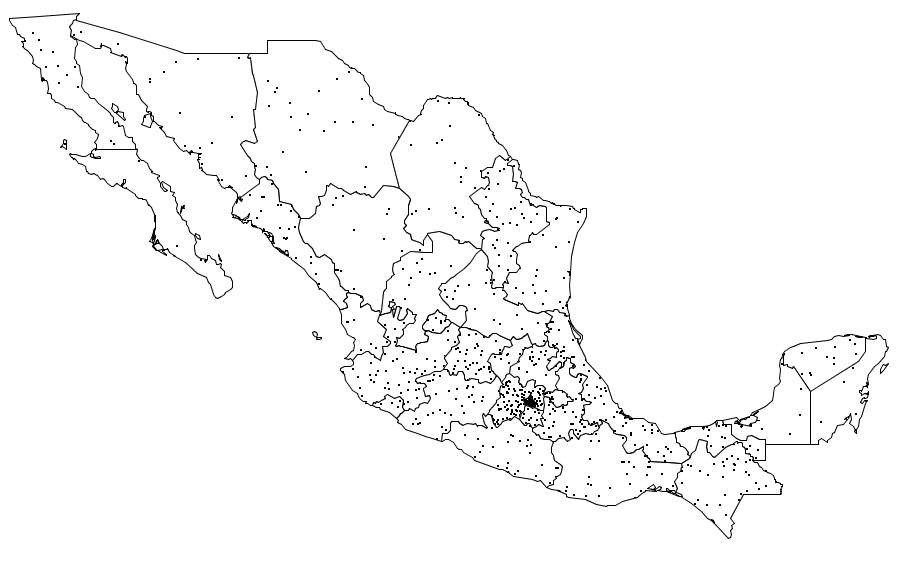
\includegraphics[width=.8\mycolumnwidth]{Mapas/MapaPuntos.png}
\caption{\small Mapa de puntos.}
\label{Fig:MapaPuntos} 
\end{figure}


\subsection{Mapas de isol�neas}\label{MapasIsolineas}\index{Mapa!de isol�neas}\index{Isol�neas}

Los mapas de isol�neas son unos de los m�s usados para la representaci�n de informaci�n cuantitativa, en particular cuando se trata de variables continuas. Se utiliza habitualmente para representar campos escalares y constituye una forma muy efectiva de incorporar esta informaci�n en un mapa, ya que puede combinarse con otros tipos de mapas y de informaci�n, debido a que, al representarse �nicamente mediante l�neas, permite la presencia de otros elementos dentro del mapa sin resultar obstrusiva.

Un mapa de isol�neas est� formado por un conjunto de l�neas, cada una de las cuales une puntos que presentan el mismo valor de la variable. Estas l�neas no pueden cruzarse, ya que ello significar�a que en un punto se presentan dos valores. El caso m�s t�pico de mapa de isol�neas son las curvas de nivel que aparecen el un mapa topogr�fico, indicando la elevaci�n del terreno. Otras variables que habitualmente se representan mediante curvas de nivel son la temperatura (en cuyo caso, las l�neas se denominan \emph{isotermas}), la presi�n (\emph{isobaras}) o el tiempo (\emph{isocronas}). En el caso de las curvas de elevaci�n, estas se conocen como \emph{isohipsas}, aunque resulta mucho m�s habitual denominarlas simplemente curvas de nivel, nombre que se emplea tambi�n por extensi�n como sin�nimo general de isol�neas.

Para una variable continua, los valores que esta puede tomar son infinitos, por lo que el n�mero de isol�neas que pueden trazarse tambi�n lo es. Por ello, es necesario seleccionar qu� isol�neas se desea representar, estableciendo clases y representando tan solo los l�mites de estas. A pesar de esta divisi�n, no resulta habitual un an�lisis complejo a la hora de establecer la distintas clases, tal y como se detall� en el apartado \ref{CreacionClases}. En su lugar, se emplean en la gran mayor�a de casos intervalos iguales, siendo el tama�o de cada clase (el rango de valores que cubre) el �nico par�metro a definir. Este par�metro es lo que se conoce como \emph{equidistancia} en un mapa de curvas de nivel.

La construcci�n de un mapa de curvas de nivel es una tarea compleja que requiere de unas t�cnicas particulares que no detallaremos aqu�. La raz�n para esto es que, dentro de un SIG, esas t�cnicas se aplican de forma distinta a trav�s de procesos como los que ya hemos visto en la parte correspondiente del libro. El problema principal para la construcci�n del mapa de isol�neas es estimar el trazado de estas a partir de valores puntuales, lo cual coincide con lo que vimos en el cap�tulo \ref{Creacion_capas_raster} acerca de los distintos m�todos de interpolaci�n. Por esta raz�n, dentro de un SIG el procedimiento a seguir ser� calcular una capa r�ster a partir de valores puntuales, y despu�s crear las isol�neas a partir de esta capa seg�n lo visto en el apartado \ref{Isolineas}, no siguiendo la metodolog�a cl�sica de creaci�n de estas a pesar de que los fundamentos te�ricos subyacentes (las t�cnicas de interpolaci�n) son los mismos en ambos casos.\index{Interpolaci�n}

Algo que si debe citarse en lo que respecta a la creaci�n de las isol�neas, ya sea con o sin la ayuda del SIG, es la diferencia entre las denominadas \emph{isaritmas} o \emph{l�neas isom�tricas} y las \emph{isopletas}. Las isartimas expresan una variable que existe como tal en aquellos puntos por los que pasa la isol�nea, como por ejemplo en el caso de la elevaci�n. Una curva de nivel de 100 metros pasa por un punto en el que la elevaci�n es exactamente igual a 100. Con otras variables, sin embargo, el valor no tiene que existir como tal en esos puntos, y la isol�nea es solo una forma de representar el comportamiento de la variable. As� sucede, por ejemplo, en valores que no ocurren en puntos, sino por unidad de �rea, y que al convertir en isol�neas dan lugar a las citadas isopletas.\index{Isaritmas}\index{Isopletas}

Imaginemos, por ejemplo, el caso de la densidad de poblaci�n. Podemos crear unas isol�neas de densidad de poblaci�n, pero no podemos medir esta en un punto. Debemos contar los habitantes en un �rea dada y despu�s dividir entre dicho �rea. El valor obtenido debemos despu�s asignarlo a un punto y con el conjunto de puntos as� obtenidos ya podremos crear las isol�nea. La diferencia en este caso es que esa unidad de �rea debe resumirse en un punto. 

En caso de que dentro de la unidad exista una distribuci�n homog�nea, podemos asignar el valor del �rea a su centro geom�trico, pero de no ser as� es necesario buscar otra localizaci�n en base a la informaci�n adicional de que dispongamos. Por ello, los mapas de isopletas presentan mayor incertidumbre que los de isaritmas, especialmente si las unidades de �rea empleadas son grandes. Aunque a efectos de su representaci�n (que es principalmente lo que estamos tratando en este cap�tulo) no existen diferencias, los aspectos que deben tenerse en cuenta a la hora de su uso y creaci�n son distintos y deben rese�arse.

A la hora de simbolizar las isol�neas, y con independencia de su tipo, la variable visual tama�o es la �nica que suele emplearse, en particular para se�alar aquellas l�neas que representan un valor m�ltiplo de una determinada cantidad y hacer as� m�s f�cil la lectura del mapa. Estas l�neas son lo que se conoce como \emph{curvas directrices}. Por ejemplo, en un mapa topogr�fico con curvas de nivel con una equidistancia de 100 metros, es habitual establecer curvas directrices cada 500 metros. Todas aquellas curvas cuyo valor asociado sea m�ltiplo de 500 se representan con un trazo m�s grueso para que puedan localizarse r�pidamente.\index{Curva!directriz}

\begin{figure}[!hbt]
\centering
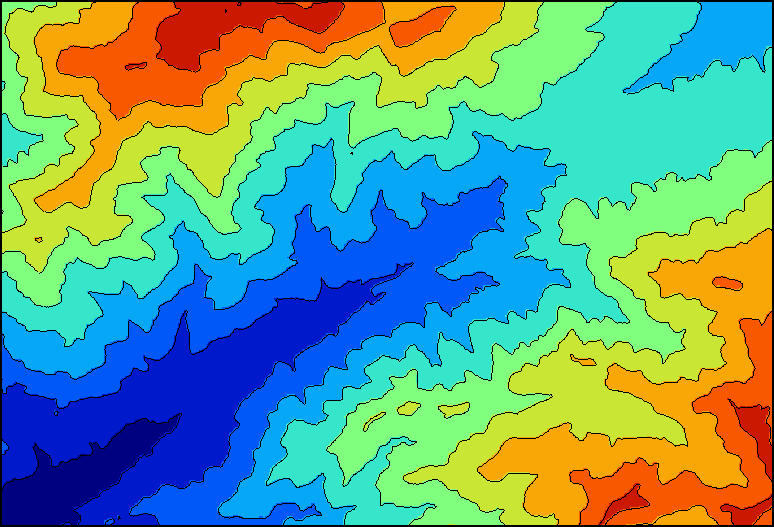
\includegraphics[width=.8\mycolumnwidth]{Mapas/Isolineas.png}
\caption{\small Mapa de isol�neas. Se ha empleado para su representaci�n tanto las l�neas como el coloreado de las franjas entre estas.}
\label{Fig:Isolineas} 
\end{figure}


El uso del color o la textura en las l�neas no es habitual como simbolog�a, ya que simbolizar los valores de cada una	 trav�s de las variables visuales resulta en este caso menos pr�ctico. Lo normal es etiquetar cada una de ellas con el valor concreto (con texto sobre la l�nea), y aprovechar el hecho de que dos l�neas consecutivas est�n separadas siempre una magnitud igual al tama�o de la clase (la equidistancia), lo cual aporta un importante contexto en lo que a los valores se refiere. 

Una forma particular de representar las isol�neas mediante color es hacerlo no sobre las l�neas, sino sobre las zonas que median entre ellas. Es decir, representar la clase en lugar del l�mite de clase. Este tipo de mapas se asemeja al mapa de coropletas (que veremos seguidamente), trat�ndose m�s de un mapa de �reas que de l�neas, por lo que se conoce como de \emph{isocoropletas}. Ambos tipos de representaci�n, mediante �reas y mediante l�neas, pueden combinarse en un �nico mapa.\index{Isocoropletas}

En la figura \ref{Fig:Isolineas} puede verse un ejemplo de mapa de isol�neas combinando las dos formas anteriores.


\subsection{Mapas de coropletas}\index{Mapa!de coropletas}

Los mapas de coropletas son utilizados muy habitualmente para representar la informaci�n geogr�fica en un SIG, y hemos visto ejemplos de ellos en otros puntos de este y otros cap�tulos. Por ejemplo, los mapas de la figura \ref{Fig:TiposIntervalosClases} son todos ellos mapas de coropletas.

En un mapa de coropletas se tiene una serie de �reas definidas, cada una de las cuales posee un valor de una variable. Este valor de la variable afecta a todo el �rea y es el que se representa por medio de alguna variable visual, normalmente el color a trav�s de su componente valor. Las zonas definidas por cada �rea tienen un significado arbitrario, no relacionado con la variable asociada. Muy frecuentemente, se utilizan limites administrativos o de gesti�n como �reas. Cada �rea conforma una unidad espacial, y el valor asociado a ella resume la variable dentro de dicho �rea. 

Precisamente por esta generalizaci�n que se da al representar mediante un �nico valor la variable dentro de cada unidad, los mapas de coropletas adolecen de ciertos inconvenientes, siendo los dos siguientes los principales:

\begin{itemize}
	\item Sensaci�n de cambio brusco en los l�mites entre �reas. Al existir una transici�n abrupta entre unidades, un mapa de coropletas puede transmitir la idea de que en esa frontera los valores de la variable cambian bruscamente, ocultando la continuidad de la variable en caso de existir esta.
	\item Homogeneidad dentro de cada �rea. La variaci�n dentro de cada �rea no se recoge, con lo que se pierde una parte de la informaci�n. El uso de unidades menores soluciona en parte este problema, aunque puede hacer el mapa m�s complejo de interpretar y puede desvirtuar la informaci�n (recordemos aqu� todo lo que vimos en el cap�tulo \ref{Analisis_espacial} y los conceptos tales como el Problema de la Unidad de �rea Modificable)\index{Problema de la Unidad de �rea Modificable}. Al mismo tiempo, las unidades pueden tener su significado particular, como por ejemplo tratarse de divisiones administrativas, con lo que el uso de otras distintas altera la informaci�n que se pretende transmitir. 	
\end{itemize}

Igualmente, debe considerarse que, en el caso de valores no normalizados, las coropletas pueden transmitir una informaci�n equivocada. Por ejemplo, si una variable representa un conteo, tal y como la poblaci�n de un conjunto de estados, el uso de coropletas no tiene en cuenta la superficie de cada una de las �reas representadas. Un mismo valor en dos unidades, una de ellas con una superficie mucho mayor a la otra, puede dar la sensaci�n de que poblacionalmente ambas zonas son similares, mientras que puede ser que una tenga una gran densidad de poblaci�n y la otra est� pr�cticamente despoblada. El valor que simbolizamos s� est� relacionado con el �rea (a mayor �rea, encontraremos m�s habitantes), y ser�a m�s adecuado representar esa densidad de poblaci�n, ya que resulta menos proclive a inducir una interpretaci�n err�nea. En general, el uso de coropletas es correcto cuando la variable ha sido normalizada, por ejemplo dividiendo el valor num�rico de cada unidad entre la superficie de esta.

En los mapas de coropletas cobra especial importancia la correcta divisi�n de clases seg�n hemos detallado dentro de este mismo cap�tulo. De entre las variables visuales, el color es la usada en la gran mayor�a de casos, en particular utilizando su componente valor, y las propias caracter�sticas de las coropletas, en particular las desventajas que ya hemos mencionado, han de considerarse a la hora establecer c�mo hacemos uso de esta variable visual para la simbolizaci�n de cada unidad. 

As�, debemos tener en cuenta que a la hora de distinguir dos colores con el mismo tono y distinto valor, si estos son muy semejantes solo resulta posible diferenciarlos cuando se sit�an el uno junto al otro, pero no cuando est�n separados y median entre ellos otros colores distintos. Aunque la variable con la que trabajemos sea continua, el mapa de coropletas no ha de exhibir dicha continuidad, por lo que no podemos contar con ella para elaborar la rampa de valores correspondiente. Mientras que en un mapa de isol�neas sabemos que los distintos colores van a aparecer de forma ordenada (en el mismo orden en el que se muestran en la leyenda), en el mapa de coropletas una unidad puede tener a su lado otra con un valor muy distinto sin que entre ellas exista una de valor intermedio, pudiendo producirse un salto de varias clases. Esto tiene como consecuencia que el n�mero de clases que podemos emplear es menor que al trabajar con isol�neas, ya que esta separaci�n espacial que puede aparecer en las distintas clases va a dificultar su diferenciaci�n.

De igual modo el uso del tono queda m�s restringido, al poder dar lugar a situaciones ambiguas. Por ejemplo, si miramos la leyenda del mapa de la figura \ref{Fig:TintasElevacion} veremos que hay dos clases con un tono blanco. Por una parte, los valores situados cerca del cero (al nivel del mar). Por otro, los situados en la parte superior de la escala, es decir, los que corresponden a mayor elevaci�n. Esto no da lugar a ambig�edad, ya que el primer caso siempre aparecer� cerca de tonos azules, mientras que el segundo se situar� cerca de los marrones. No puede ser de otro modo, ya que equivaldr�a a que las curvas de nivel pudieran cortarse entre s�, lo cual sabemos que no es posible. El contexto de los colores circundantes sirve para eliminar la ambig�edad. En el mapa de coropletas, al no suceder necesariamente as�, la ambig�edad permanecer�a y har�a imposible discernir el significado de la simbolog�a. En el caso de las isocoropletas, en la que la contig�idad espacial s� implica tambi�n contig�idad de clases, s� pueden utilizarse este tipo de esquemas, como ya vimos en la figura \ref{Fig:Isolineas}.

Por todo lo anterior, el uso de la componente valor es preferible frente al uso del tono a la hora de crear un mapa de coropletas para representar informaci�n cuantitativa.

\subsection{Otros tipos de mapas}

Existen muchos otros tipos de mapas, adecuados para representar tipos particulares de informaci�n. A pesar de su utilidad, son mucho menos frecuentes, especialmente dentro del �mbito SIG, ya que su implementaci�n no es habitual y no resulta com�n crearlos con las herramientas usuales de estos. Algunos de estos tipos de mapas que resulta de inter�s rese�ar son los siguientes:

\begin{itemize}
	\item Mapas dasim�tricos. Los mapas dasim�tricos tratan de evitar las deficiencias de los mapas de coropletas, en los que los l�mites de las distintas �reas representadas no tienen relaci�n con la variable con la que se trabaja, siendo limites arbitrarios tales como divisiones administrativas o territoriales. En los mapas dasim�tricos las divisiones obedecen a la propia geograf�a de la variable. El principal inconveniente de estos mapas es el mayor esfuerzo que su preparaci�n exige, as� como el mayor conocimiento de la variable que resulta necesario para poder definir las distintas zonas del mapa. Tradicionalmente se han empleado para representar la densidad de poblaci�n, siendo poco usados para otras variables.\index{Mapa!dasim�trico}
	\item Mapas de flujo. Los mapas de flujos representan movimientos de alg�n tipo de elemento, como por ejemplo las exportaciones de un producto o los desplazamientos de tropas en una campa�a militar. El mapa de flujo aporta informaci�n sobre c�mo se produce la distribuci�n del elemento que se desplaza, la proporci�n o magnitud en que lo hace, as� como tambi�n la ruta seguida, aunque este �ltimo factor no es habitualmente prioritario y suele representar m�s con car�cter esquem�tico (indicando la relaci�n entre los puntos de partida y destino del movimiento) que como verdadera informaci�n geogr�fica sobre el trayecto en cuesti�n. Algunos de los mejores ejemplos de mapas de flujo son los creados por Charles Joseph Minard (1781--1870), ingeniero franc�s pionero en su creaci�n. Uno de esos mapas puede verse en la figura \ref{Fig:MapaFlujo}.\index{Mapa!de flujo}
	
\begin{figure}[!hbt]
\centering
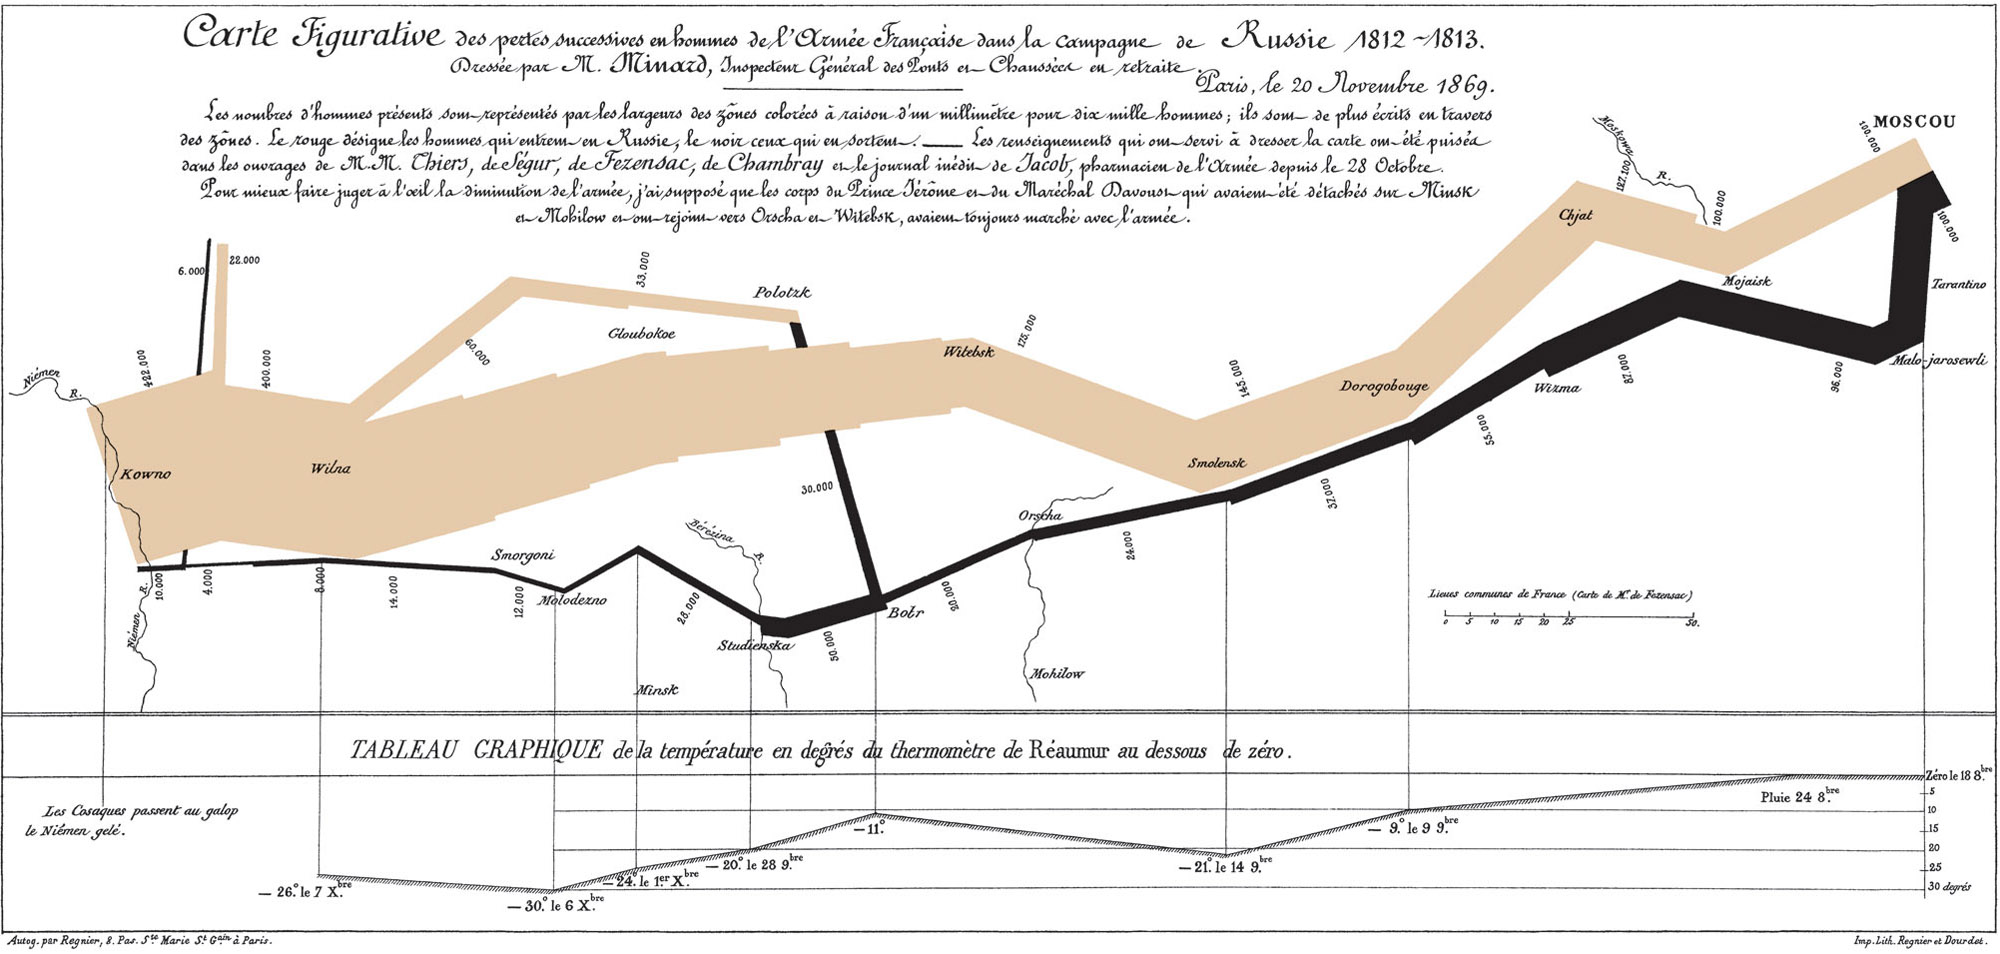
\includegraphics[width=\mycolumnwidth]{Mapas/MapaFlujo.png}
\caption{\small Mapa de flujo de Charles Joseph Minard sobre la campa�a de Napole�n en Rusia.}
\label{Fig:MapaFlujo} 
\end{figure}

\item Cartogramas. En los cartogramas, la informaci�n cualitativa se transmite mediante la modificaci�n de las unidades de superficie, que se distorsionan para representar con su tama�o la magnitud de la variable en cuesti�n. Es decir, la variable visual tama�o se aplica directamente sobre las distintas unidades de superficie. En la figura \ref{Fig:Cartograma} puede verse un ejemplo de cartograma en el que los pa�ses de la uni�n europea se representan de tal modo que su tama�o es proporcional a su poblaci�n. La densidad de poblaci�n se incorpora mediante el tono en que se representa cada uno de esos pa�ses. Aquellos pa�ses con una mayor densidad de poblaci�n son los que sufren m�s distorsi�n en la representaci�n de sus contornos.\index{Cartograma} 

\begin{figure}[!hbt]
\centering
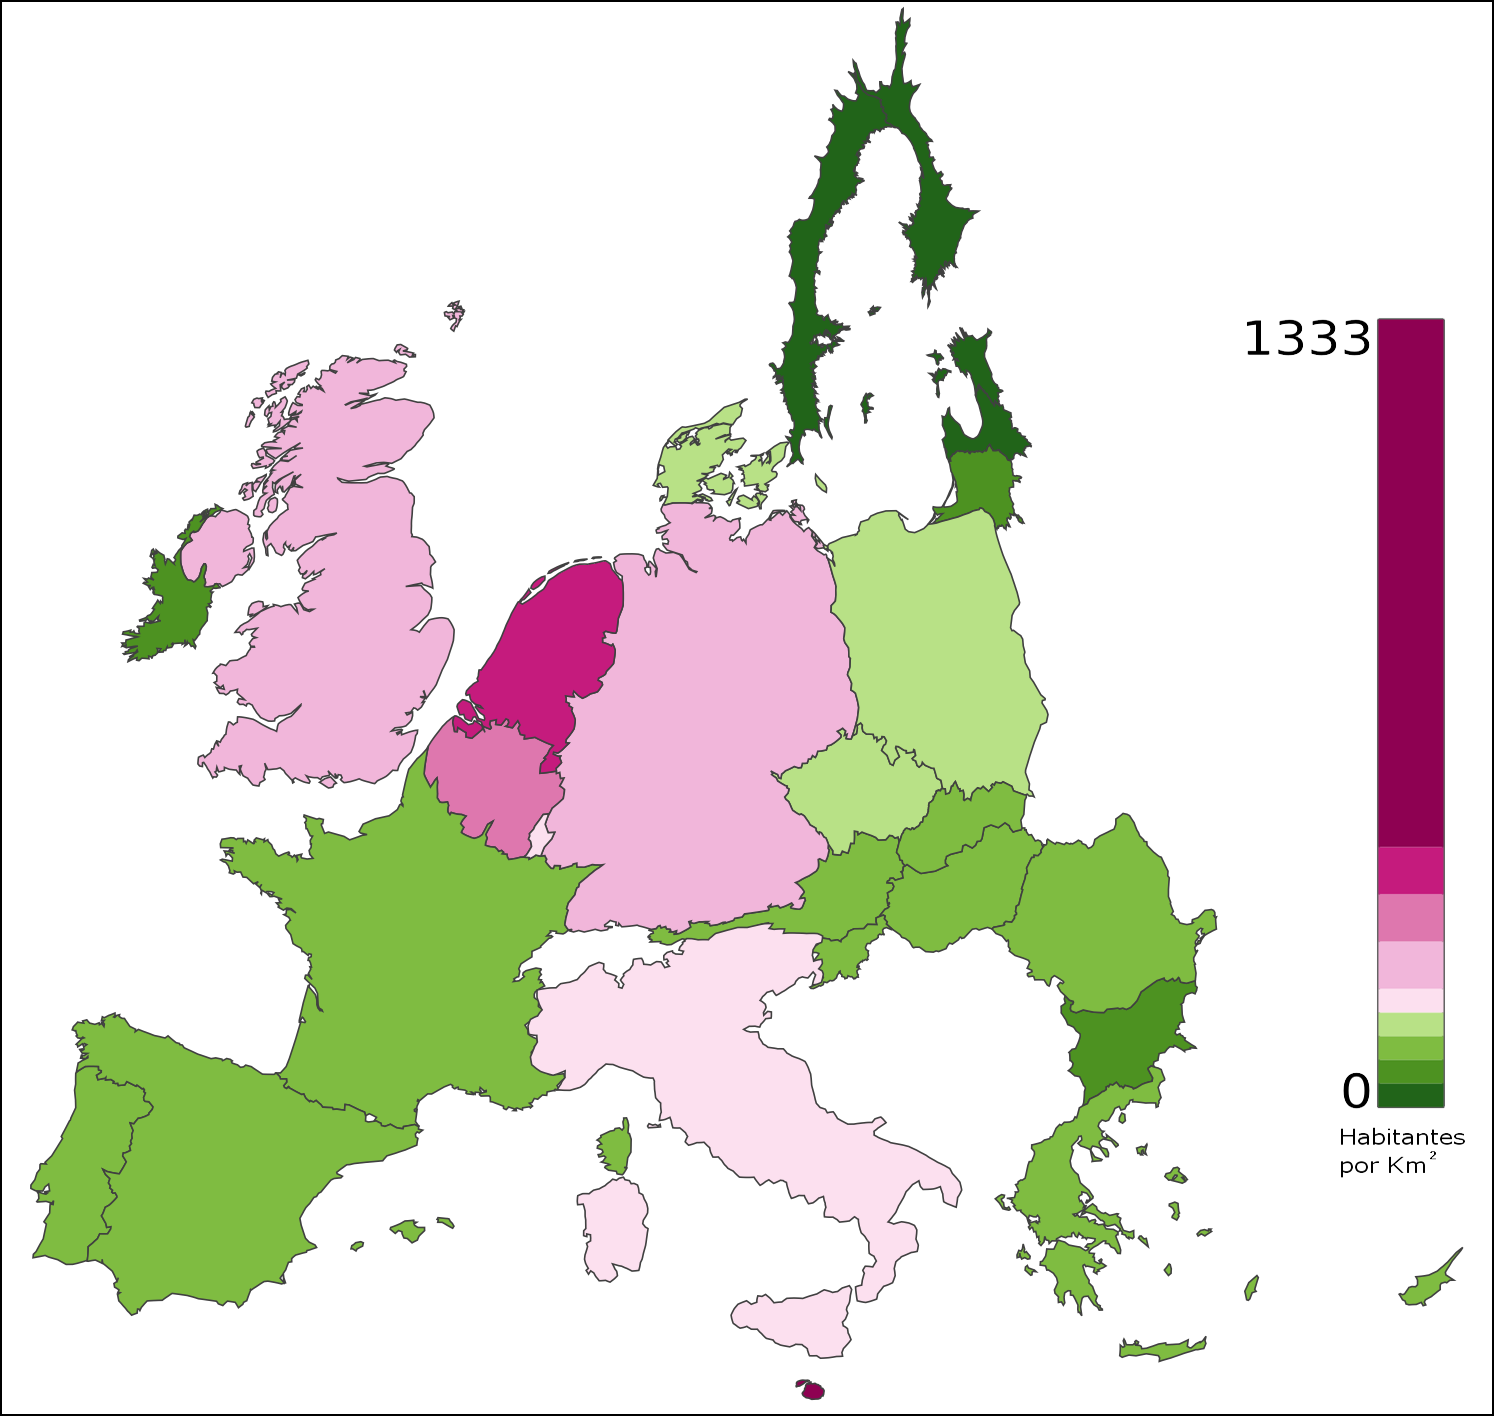
\includegraphics[width=.6\mycolumnwidth]{Mapas/Cartograma.png}
\caption{\small Un ejemplo de cartograma (Adaptado de Wikipedia).}
\label{Fig:Cartograma} 
\end{figure}

\end{itemize}

\section{Resumen}

Hemos visto en este cap�tulo c�mo un mapa constituye una forma de comunicaci�n visual, y c�mo en esa comunicaci�n existen una serie de factores a tener en cuenta para que la transmisi�n de la informaci�n entre emisor y receptor sea �ptima. De especial relevancia en este sentido es prestar atenci�n a este �ltimo y tener siempre en cuenta el prop�sito del mapa que creamos.

Distinguimos dos tipos de cartograf�a: la cartograf�a de base y la tem�tica. Esta �ltima es la que crearemos con m�s frecuencia en un SIG. Las formas de cartograf�a tem�tica est�n muy relacionadas con las caracter�sticas de la variable. Para el caso de variables cuantitativas, es importante agrupar adecuadamente los distintos valores en clases. Existen diversas formas de delimitar los intervalos correspondientes, siendo las m�s habituales el uso de intervalos iguales, intervalos naturales o intervalos basados en la media y la desviaci�n t�pica de los valores en cuesti�n.

Dentro de los tipos de mapas tem�ticos m�s importantes encontramos los mapas de puntos, de s�mbolos proporcionales, de isol�neas y de coropletas, cada uno de ellos con sus caracter�sticas particulares. Los mapas de isol�neas son especialmente indicados para la representaci�n de variables continuas, mientras que por su parte las variables de tipo razones se representan de forma especialmente adecuada mediante los mapas de puntos. 

A la hora de componer un mapa existen diversos elementos que deben a�adirse para facilitar su interpretaci�n. Adem�s de conocer la funci�n de cada uno, es importante saber c�mo situar estos sobre el lienzo del mapa, aprovechando correctamente el espacio e integr�ndolos adecuadamente.




\chapter{La visualizaci�n en t�rminos SIG}\label{Visualizacion_SIG}

\begin{keypoints}
�Qu� par�metros puedo configurar en la representaci�n de una capa vectorial? $\bullet$ �Y de una capa r�ster? $\bullet$ �C�mo puedo combinar varias capas de la mejor forma posible? $\bullet$ �C�mo elaboro una vista tridimensional? $\bullet$ �Qu� otros elementos pueden emplearse para enriquecer una representaci�n en un SIG?
\end{keypoints}

\bigskip

\begin{intro}
Ahora que ya conocemos la teor�a del dise�o cartogr�fico y sus ideas principales, es momento de aplicar esto a los SIG y ver en qu� medida un SIG nos permite aplicar esas ideas. El objetivo de este cap�tulo es facilitar la aplicaci�n de todo lo visto en los anteriores, para mejorar as� nuestro trabajo con un SIG. Se trata de un cap�tulo eminentemente pr�ctico en el que veremos la visualizaci�n no desde un punto de vista conceptual, sino directamente sobre el SIG, y aprenderemos c�mo usar este para lograr crear mejores mapas y, en general, mejores visualizaciones de todo tipo de datos susceptibles de ser incorporados en un SIG.
\end{intro}


\section{Introducci�n}

El SIG es nuestro �til para visualizar la informaci�n geogr�fica y, como hemos visto, un �til muy potente y con numerosas posibilidades. Conocemos ya sus capacidades y limitaciones, pero no sabemos todav�a c�mo debemos trabajar con estas a la hora de crear una representaci�n visual y, sobre todo, desconocemos la forma en que las particularidades de la informaci�n geogr�fica dentro de un SIG afectan a su visualizaci�n.

El concepto de capa, que resulta vital para otras tareas tales como el an�lisis, va a tener de igual modo una influencia directa en la creaci�n de representaciones a partir de los datos de que disponemos, ya que la interpretaci�n de estos datos est� condicionada inevitablemente al modelo de datos empleado. Por ello, veremos en este cap�tulo los conceptos que ya conocemos de otros anteriores, pero aplicados al caso particular de aplicarlos dentro de un SIG, empleando las herramientas que este habitualmente incluye para esa tarea.

Puesto que conocemos ya un buen conjunto de operaciones sobre los datos espaciales, y estas operaciones forman parte integrante del SIG al igual que la visualizaci�n, estudiaremos asimismo c�mo aprovechar algunas de estas operaciones de cara a la visualizaci�n de informaci�n geogr�fica. Es aqu� donde reside una de las grandes virtudes del SIG, en que sus distintas capacidades est�n conectadas y son accesibles desde un mismo entorno. Hacer m�s patente esa relaci�n entre ellas y ampliar as� las posibilidades que un mismo juego de datos ofrece para ser representado es uno de los objetivos de este cap�tulo. 

En conjunto, las capacidades que ofrece un SIG, incluso si en muchos casos no alcanzan la funcionalidad necesaria para satisfacer al cart�grafo profesional, permiten expandir las posibilidades de representaci�n de una capa cualquiera y obtener visualizaciones distintas a las que son  habituales en un mapa cl�sico. Del mismo modo que una aplicaci�n CAD ampl�a las posibilidades del arquitecto o ingeniero a la hora de crear planos o realizar dise�os industriales, o un programa de animaci�n abre nuevos horizontes para un dibujante, los SIG expanden las posibilidad de creaci�n y uso de cartograf�a para todo aquel que requiera visualizar la informaci�n geogr�fica.

Cuando la informaci�n geogr�fica se presenta en pantalla y dentro del contexto de la aplicaci�n SIG correspondiente, lleva asociada adem�s una interactividad de la que un mapa impreso carece, circunstancia que tambi�n debe tenerse en cuenta. As�, junto a las ideas b�sicas que ya hemos desarrollado en otros puntos dentro de esta parte del libro, es necesario a�adir algunas adicionales para cubrir toda la gama de posibles resultados visuales que ahora encontramos gracias a los SIG.

Adem�s de esa representaci�n habitual de capas que constituye la adaptaci�n de la cartograf�a cl�sica al entorno de un SIG, otras formas de visualizaci�n que encontramos en estos son novedosas y no tienen un equivalente en aquella. Aunque su relevancia es variable, algunas de ellas representan una parte importante de las funcionalidades actuales de los SIG, por lo que las trataremos por separado para ver c�mo complementan a las herramientas de visualizaci�n habituales y c�mo se integran con estas.


\section{Visualizaci�n de capas vectoriales}

La visualizaci�n de capas vectoriales en el seno de un SIG es similar a la labor de la cartograf�a cl�sica, en cuanto a que los objetos que se representan son del mismo tipo, esto es, objetos geom�tricos en forma de puntos, l�neas y pol�gonos. A diferencia de las capas r�ster, que no tienen un equivalente en un mapa cl�sico (no es probable que hayas visto un mapa previo a la aparici�n de los SIG con un aspecto como las im�genes de, por ejemplo, la figura \ref{Fig:RepresentacionRaster}), las capas vectoriales guardan mucha similitud con los elementos que un cart�grafo cl�sico plasma en un mapa. Las geometr�as de las capas vectoriales son los objetos b�sicos sobre los que el cart�grafo aplica las variables visuales seg�n vimos en el cap�tulo \ref{Conceptos_basicos_visualizacion}, y por tanto la manera de proceder es similar. Las herramientas que el SIG proporciona son aquellas que permiten modificar las variables visuales en funci�n de las caracter�sticas asociadas a cada geometr�a a representar.

Un papel destacado en la visualizaci�n lo juega la tabla de atributos, ya que es la que contiene esas caracter�sticas que son necesarias para saber \emph{c�mo} representar cada objeto. El SIG provee la conexi�n entre los valores de los atributos y la representaci�n visual, de forma que se interpretan aquellos para poder obtener los distintos tipos de mapas que ya conocemos del cap�tulo \ref{El_Mapa}.

Al igual que el tipo de informaci�n es importante para escoger el tipo de mapa a crear o la variable visual a emplear para la representaci�n, el tipo de datos ha de estar correctamente definido en la tabla de atributos para poder emplearse como tal. Es decir, ha de ser coherente con la informaci�n que recoge.

Los atributos pueden contener en ocasiones no un valor que al interpretarse se convierta en una cualidad dada de una variable visual, sino esa cualidad directamente. En el caso de capas procedentes de aplicaciones CAD\index{CAD}, es habitual que estas contengan alg�n campo con el color que ha de emplearse para representar esa capa, que puede venir indicado como un c�digo que se deber� transformar despu�s en el color correspondiente, o bien expresado directamente como el valor RGB de dicho color.

Respecto a las geometrias, es interesante hacer ver que, aunque los objetos geom�tricos que se representan son del mismo tipo que los objetos con los que trabaja el cart�grafo cl�sico, no ha de existir siempre obligatoriamente una identificaci�n directa entre ambos. En otras palabras, el cart�grafo puede pintar un conjunto de l�neas no mediante una l�nea sino como un conjunto de pol�gonos entre l�neas, tal y como sucede en el mapa de isol�neas de la figura \ref{Fig:Isolineas}. Tanto el cart�grafo cl�sico como su equivalente moderno que emplea un SIG parten los dos de un conjunto de l�neas, pero su forma de operar es distinta. \index{Isol�neas}

En un mapa cl�sico, se trazan las l�neas y despu�s se rellena con los colores correspondientes. En el SIG, no existe la posibilidad de <<rellenar>>, ya que �nicamente pueden aplicarse las variables visuales a las entidades, y el espacio intermedio entre l�neas no es ninguna entidad que tengamos almacenada en la capa. No obstante, crear esa representaci�n resulta perfectamente posible en un SIG, aunque con un planteamiento distinto.

Puesto que queremos representar objetos de superficie, necesitamos una capa de pol�gonos. Obtener esta no debiera resultarnos complicado si conocemos las rutinas que vimos en la parte de procesos, que permiten convertir capas vectoriales en capas r�ster, y viceversa. Podr�amos, por ejemplo, rasterizar la capa de l�neas, aplicar una reclasificaci�n de sus valores para que queden en clases de la misma amplitud que la equidistancia de las isol�neas, y despu�s vectorizar esas clases para obtener los pol�gonos que ya podr�amos representar y colorear adecuadamente. M�s adecuado es, no obstante, representar directamente la capa r�ster as� obtenida, sin necesidad siquiera de reclasificarla, ya que las clases las aplicar�amos en la visualizaci�n directamente. Esa es la metodolog�a empleada para obtener la representaci�n de la figura \ref{Fig:Isolineas}, cuyo resultado, como puede verse, es visualmente muy satisfactorio.

Conviven en la representaci�n tanto una capa r�ster como una vectorial. Lo relevante de este hecho es darse cuenta de las posibilidades que el SIG nos ofrece con sus funciones de an�lisis y mediante los procesos que hemos visto en una parte anterior del libro, y que pueden emplearse de igual modo para elaborar representaciones distintas. Ello aporta al SIG una flexibilidad que ha de aprovecharse cuando las capacidades de representaci�n puramente dichas no nos ofrezcan la funcionalidad que necesitamos. 

\subsection{Etiquetado}

El etiquetado representa una de las tareas m�s complejas a la hora de crear un mapa, ya sea con la ayuda de un SIG o sin ella, estim�ndose que puede llevar aproximadamente un 50\% del tiempo total de creaci�n de un documento cartogr�fico \cite{Morrison1980Wiley}. La experiencia del buen cart�grafo queda patente en su trabajo con las etiquetas, pues es en esta labor donde m�s necesaria se demuestra, y en la que el criterio personal cobra una mayor importancia. Siendo as�, es l�gico pensar que este es asimismo uno de los procesos en los que m�s dif�cil resulta proveer una soluci�n automatizada, ya que trasladar al ordenador ese buen hacer del cart�grafo profesional no es en absoluto sencillo. Por ello, aunque un SIG puede incorporar herramientas para ayudar en el etiquetado, una gran parte de este trabajo sigue siendo necesario realizarla manualmente, y es por esta raz�n que conocer algunas ideas b�sicas al respecto es b�sico si queremos elaborar cartograf�a de una cierta calidad, ya que el SIG por s� mismo no va a poder llevar a cabo esta tarea de forma autom�tica.

En esta secci�n vamos a ver algunas ideas sobre etiquetado como parte de la visualizaci�n de capas vectoriales, ya que es en estas en las que verdaderamente tiene sentido esta labor.

La premisa fundamental del etiquetado es situar las etiquetas de tal modo que estas no se solapen y que sea inmediato asociar su nombre al objeto geogr�fico que designan, as� como a la importancia y propiedades de este. Para ello, necesitamos tres tipos de informaci�n a extraer de esos objetos:

\begin{itemize}
	\item D�nde situar la etiqueta.
	\item Qu� poner en la etiqueta.
	\item C�mo ponerlo.	
\end{itemize}

Trat�ndose de capas vectoriales, toda esta informaci�n la extraeremos tanto de la geometr�a como de la tabla de atributos asociada. La m�s obvia es la relativa a qu� debe ponerse en la etiqueta, que simplemente se tomar� de alguno de los campos de la tabla que contenga los nombres de los distintos objetos.

Respecto a la posici�n, esta vendr� definida por la geometr�a y su georreferenciaci�n, aunque solo parcialmente. La geometr�a nos da una indicaci�n de la zona aproximada en la que debe situarse la etiqueta, ya que obviamente esta debe encontrarse a cerca del objeto al que hace referencia, pero no constituye una informaci�n suficiente, al menos para obtener un etiquetado �ptimo m�s all� de la configuraci�n m�s trivial. 

Por ejemplo, en el caso de puntos cercanos, situar la etiqueta de estos centrada exactamente en cada uno de ellos  har� que se solapen y oculten adem�s a los propios puntos. Es necesario colocarlas cada una de ellas alejadas de los puntos en direcciones contrarias, para que no interfieran entre s�. La localizaci�n por tanto, no depende �nicamente de las coordenadas del objeto, sino tambi�n de las de los objetos circundantes. Buscar una disposici�n que evite estos solapes es una tarea en apariencia simple, pero compleja desde el punto de su implementaci�n\footnote{Para el lector con curiosidad acerca de los algoritmos de etiquetado, baste citar que, salvo en el caso de una soluci�n trivial, se trata de un problema de tipo NP--Hard.\index{NP--Hard}}. Aun as�, est� presente en los SIG en mayor o menor medida, y en el caso de puntos, los resultados que se obtienen son de una calidad aceptable. El paso a otro tipo de geometr�as, donde es necesario considerar otra serie de par�metros, hace aparecer unas circunstancias m�s dif�ciles de tratar, y la labor directa del cart�grafo es mucho m�s necesaria.

En el caso de capas de l�neas, la posici�n de las etiquetas debe seguir el trazado de las l�neas y su orientaci�n, existiendo, no obstante, diversas opciones en lo que respecta a la posici�n con respecto a la propia l�nea. La l�nea ya no es un objeto puntual y no existe por tanto una coordenada �nica que utilizar. El punto medio de la l�nea es la soluci�n m�s inmediata como punto de referencia, pero no necesariamente la mejor. Pueden existir otras zonas a lo largo de la l�nea que resulten m�s relevantes y en las que sea m�s adecuado situar la etiqueta. En el caso de l�neas muy largas, es conveniente repetir el nombre varias veces a lo largo de esta, para que no sea necesario seguirla hasta encontrar su nombre.

En el caso de l�neas que se entrecruzan (calles, r�os, etc.), es importante evitar las ambig�edades. No es conveniente etiquetar una l�nea siempre que exista un cruce, pero un emplazamiento adecuado puede resultar suficiente para aclarar a qu� l�nea hace referencia una etiqueta. Esto puede verse en la figura \ref{Fig:EtiquetasLineas}. En ambos casos, la etiqueta hace referencia al cauce que procede de la parte superior, que es el principal de los dos que confluyen, y por tanto tambi�n el que da nombre al segmento posterior al cruce. En el caso a), la mayor similitud en las direcciones puede inducir sin embargo a pensar que el nombre hace referencia al cauce despu�s de la intersecci�n y al segmento horizontal antes de esta. Si el etiquetado de este segmento horizontal, que es un cauce de nombre distinto, no se encuentra suficientemente cerca del cruce, puede entonces pensarse que la etiqueta hace referencia a �l tambi�n lo cual no es adecuado. Un emplazamiento tal como el mostrado en el caso b) aclara esta situaci�n de forma elegante.

\begin{figure}
\centering
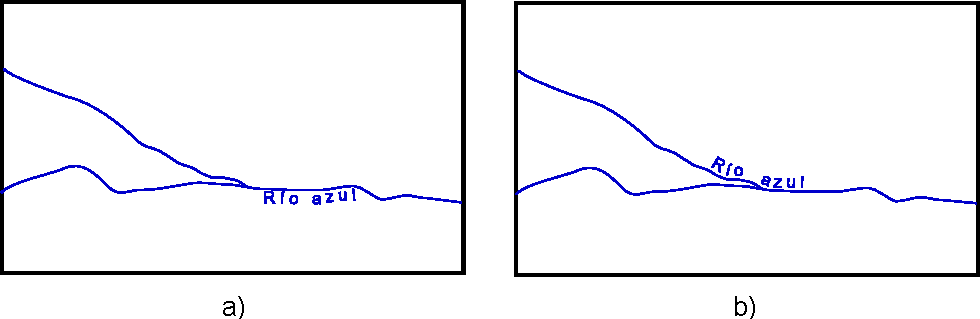
\includegraphics[width=\mycolumnwidth]{Visualizacion_SIG/EtiquetasLineas.pdf}
\caption{\small La posici�n de la etiqueta sobre una l�nea en un cruce puede dar lugar a ambig�edades (a) o a situaciones bien definidas (b).}
\label{Fig:EtiquetasLineas} 
\end{figure}

Para el caso particular de las isol�neas, se recomienda situar la etiqueta sobre la propia l�nea, ya que facilita su lectura, especialmente en el caso de que aparezcan varias isol�neas separadas por poca distancia, como puede verse en la figura \ref{Fig:EtiquetasIsolineas}. Adem�s, deben situarse las etiquetas de las isol�neas contiguas de tal forma que puedan leerse conjuntamente, para que sea sencillo interpretarlas en conjunto y apreciar sin dificultad la equidistancia y la direcci�n en la que los valores aumentan o disminuyen.

\begin{figure}
\centering
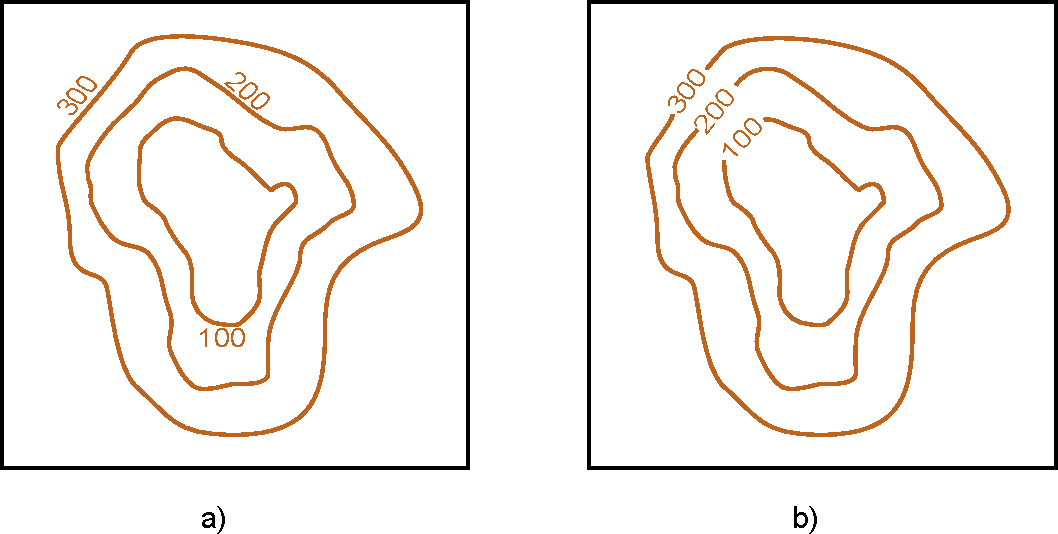
\includegraphics[width=.8\mycolumnwidth]{Visualizacion_SIG/EtiquetasIsolineas.pdf}
\caption{\small Etiquetado de isol�neas. Deben situarse las etiquetas cercanas entre s� y sobre la l�nea, como en el ejemplo b)}
\label{Fig:EtiquetasIsolineas} 
\end{figure}

Si la l�nea presenta cambios de direcci�n bruscos, es dif�cil hacer que la etiqueta siga la l�nea sin tener un aspecto <<roto>>. Suavizar las l�neas es una opci�n en este caso, al menos para usarlas como l�neas base sobre las que situar las etiquetas.

En el caso de pol�gonos, existe igualmente el problema de seleccionar un punto para emplazar la etiqueta. El centroide del pol�gono es la opci�n m�s inmediata, aunque no necesariamente ha de caer dentro de este si se trata de un pol�gono c�ncavo, e incluso en ese caso puede no resultar la mejor elecci�n.

Como puede verse, para tomar este tipo de decisiones es necesario tener en cuenta no solo la posici�n del objeto y la de los circundantes, sino tambi�n <<entender>> qu� es lo que estamos representando y qu� otra informaci�n tenemos alrededor, lo cual resulta m�s complejo de trasladar a la aplicaci�n SIG para que pueda hacerlo de forma autom�tica. Tal y como coment�bamos, la intervenci�n del cart�grafo es en este caso imprescindible para incorporar este tipo de circunstancias y aportar al mapa la calidad que un mecanismo autom�tico de etiquetado no es capaz por el momento de ofrecer.

Una vez se ha definido la posici�n m�s adecuada para las etiquetas, es necesario decidir c�mo representar cada una de ellas. Algunas etiquetas son m�s relevantes que otras, y la claridad con la que una etiqueta transmite su informaci�n depende en gran medida de c�mo esta se escribe. Los conceptos de la tipograf�a son de relevancia en este caso, y son a los que debemos acudir. He aqu� algunos de ellos.

\index{Variables visuales}
\begin{itemize}
	\item El uso de las variables visuales que conocemos es limitado en el caso de las etiquetas y, salvo el tama�o, no suelen emplearse para diferenciar unas de otras o darles m�s importancia. 
	\item El uso del tono o el valor debe llevarse a cabo con precauci�n. La legibilidad de la etiqueta, no obstante, est� en relaci�n con el fondo, ya que el color de este puede dificultar su lectura, y en esta situaci�n es a veces necesario usar uno u otro tono para garantizar esa legibilidad. La etiqueta siempre est� en un primer plano, por lo que el resto del mapa bajo ella y en su entorno forma parte del fondo. Como ya vimos, un adecuado contraste entre fondo y figura es importante, por lo que variar el color de una etiqueta puede a veces ser necesario para que esta pueda leerse correctamente. 
	
	Algunos elementos se etiquetan sistem�ticamente con colores establecidos, como en el caso de los r�os, del mismo color azul que la propia geometr�a de estos.
	\item El tama�o es la forma principal de jerarquizar las etiquetas y darles m�s importancia. Se puede aplicar directamente sobre el tama�o de la fuente, aunque tambi�n es posible hacerlo sobre el grosor (fuente normal o negrita).
	\item El uso de may�sculas o min�sculas sirve igualmente para conceder m�s importancia a unas u otras etiquetas.
	\item La separaci�n entre caracteres se puede modificar para hacer que la etiqueta cubra un espacio mayor a lo largo de un objeto lineal, eliminando en ocasiones la necesidad de un etiquetado m�ltiple de esta. Un espaciado mayor tambi�n aporta mayor �nfasis a la etiqueta. Tambi�n se puede optar por un espaciado menor en etiquetas menos importantes, o en zonas con alta densidad, para disminuir el espacio que estas ocupan y evitar solapes.
	\item El uso de fuentes art�sticas o decorativas no es recomendable. Se deben utilizar fuentes sencillas y que sean lo m�s legibles posible.	
\end{itemize}

La informaci�n necesaria para realizar todos estos ajustes a las etiquetas debe estar contenida en la tabla de atributos de la capa. As�, podemos incluir en esta campos que indiquen el �ngulo en el que se escribe la etiqueta, el tama�o a utilizar o la separaci�n de car�cter, entre otras caracter�sticas. Incluso la propia posici�n puede especificarse de esta forma. En caso de existir estos valores, el SIG los usar� en lugar de aquellos que resultar�an de la aplicaci�n de los algoritmos de etiquetado autom�tico de que disponga, entendiendo que el ajuste manual es de mejor calidad. Dado que este tipo de configuraci�n es habitual si se desea crear un mapa de calidad, algunos SIG permiten la incorporaci�n de capas de etiquetado, que contienen toda la informaci�n necesaria para el establecimiento de etiquetas, de forma que estas se incorporan al mapa por separado y no a partir de los objetos a los que hacen referencia y sus atributos. Esta manera de proceder, no obstante, es m�s laboriosa.

En resumen, la tarea de etiquetar un mapa es compleja y normalmente va a requerir una cierta cantidad de trabajo manual por parte del creador del mapa. Los SIG disponen de herramientas para automatizar una parte de este trabajo, aunque la implementaci�n de estas herramientas es muy variada, y encontramos desde aplicaciones con poco m�s que un sistema trivial de etiquetado a sistemas complejos altamente configurables. En cualquier caso, incluso en el m�s avanzado de los programas, es muy probable que debamos llevar a cabo alg�n tipo de modificaci�n o que debamos especificar manualmente algunos de los par�metros que el SIG emplea para llevar a cabo un etiquetado autom�tico o semi--autom�tico.


\section{Visualizaci�n de capas r�ster}

Las capas r�ster son, en lo que a visualizaci�n respecta, las que resultan m�s novedosas si las comparamos con lo que encontramos en un mapa cl�sico. A diferencia de las capas vectoriales, compuestas por elementos que s� aparecen en estos mapas y cuya estructura l�gica se asemeja mucho a la estructura gr�fica de un mapa a base de s�mbolos puntuales, lineales y de superficie, las capas r�ster dan  lugar a representaciones que no resulta tan frecuente ver en la cartograf�a cl�sica. 

La cartograf�a cl�sica, especialmente la relativa a lo que denomin�bamos cartograf�a base, se encarga de recoger qu� es lo que hay en una determinada porci�n de terreno, llevando esto a cabo mediante la representaci�n de una serie de objetos que se corresponden con aquello que encontramos en ese terreno. Este es un enfoque mucho m�s acorde con el modelo de representaci�n vectorial, y m�s alejado del modelo r�ster. La representaci�n gr�fica de variables continuas, las cuales se aprovechan plenamente con el modelo r�ster, no es objeto tradicionalmente de la cartograf�a, y de serlo se representan mediante geometr�as simples, tales como las l�neas en un mapa de isol�neas. Es decir, para el cart�grafo cl�sico, e independientemente del tipo de variable a representar, los datos se manejan en un modelo de representaci�n de tipo vectorial.

Esto obedece principalmente al gran detalle que tiene una capa r�ster, el cual hace inviable el uso de un planteamiento similar a la hora de crear un mapa sin la ayuda de un SIG. El cart�grafo puede trazar unas isol�neas sin dificultad para representar la topograf�a, pero dividir el lienzo del mapa en miles de peque�os cuadrados y colorear cada uno de un color seg�n su elevaci�n es por completo inviable. M�s a�n, disponer de los datos a representar en este caso (que constituir�an un MDE), resulta tambi�n imposible si no se dispone de un ordenador para calcularlo.

Por todo ello, las capas r�ster nos van a permitir crear representaciones algo distintas a las habituales en la cartograf�a cl�sica y, aunque las diferencias conceptuales con respecto a la visualizaci�n de capas vectoriales son pocas, hay algunas ideas que deben detallarse.

Formalmente, y al igual que de cara a su an�lisis, podemos considerar una capa r�ster como una capa vectorial de pol�gonos (cuadrados en este caso). No obstante, e igual tambi�n que para el an�lisis, la regularidad de la capa r�ster es el elemento clave que aporta la diferencia m�s importante, y en el que reside la particularidad de ese modelo de representaci�n.

Si a cada uno de los pol�gonos cuadrados de los que se compone una capa r�ster le asignamos un color, podemos considerar que el mapa resultante es equivalente a un mapa de coropletas, aunque con tres caracter�sticas peculiares: las unidades tienen un mismo tama�o todas ellas, este tama�o es normalmente muy peque�o y tiene dimensiones muy reducidas en la representaci�n, y las unidades est�n situadas de forma regular en una malla. Estas caracter�sticas hacen que algunos de los inconvenientes de los mapas de coropletas no se presenten, y permiten un uso distinto de las variables visuales.

Por ejemplo, el uso del tono como variable ordenada, que ya vimos que en ciertos casos s� resulta adecuado, se puede dar en las capas r�ster. Como ya se mencion� al desarrollar las variables visuales, puedes encontrar abundantes ejemplos de representaciones as� en los cap�tulos de la parte dedicada a procesos dentro de este libro. La regularidad de la malla de celdas, junto con la autocorrelaci�n espacial y la continuidad de una variable a representar, hacen que cada celda est� rodeada de otras de valores similares, lo que aporta tambi�n una continuidad visual que puede aprovecharse para emplear esquemas ordenados basados en el tono.\index{Autocorrelaci�n espacial}	

Tanto si se usa el valor como si se usa el tono, otra de las consecuencias de la estructura de una capa r�ster, y en particular del peque�o tama�o de sus celdas es el hecho de que resulta de inter�s aumentar el n�mero de clases en que dividimos los valores de la variable para asignarles el correspondiente valor o tono como variable visual. La mayor resoluci�n espacial con la que trabajamos se puede acompa�ar tambi�n de una mayor resoluci�n crom�tica para obtener representaciones de mayor riqueza.

Mencion�bamos en el apartado \ref{CreacionClases} que no se recomienda un n�mero de clases mayor de 7 u 8, ya que har�a complejo el identificar cada una de ellas en la leyenda y conocer la cantidad exacta que se representa. Ello no significa, sin embargo, que el ojo humano no pueda distinguir m�s de 8 valores distintos de un tono dado. Si extendemos el n�mero de clases, podemos lograr un efecto de transici�n suave entre los colores de las distintas celdas y eso, aunque no facilite la identificaci�n de un color concreto con su valor asociado de la variable representado, crea una representaci�n mucho m�s informativa. Puede verse esto claramente en la figura \ref{Fig:RepresentacionRaster}

\begin{figure}
\centering
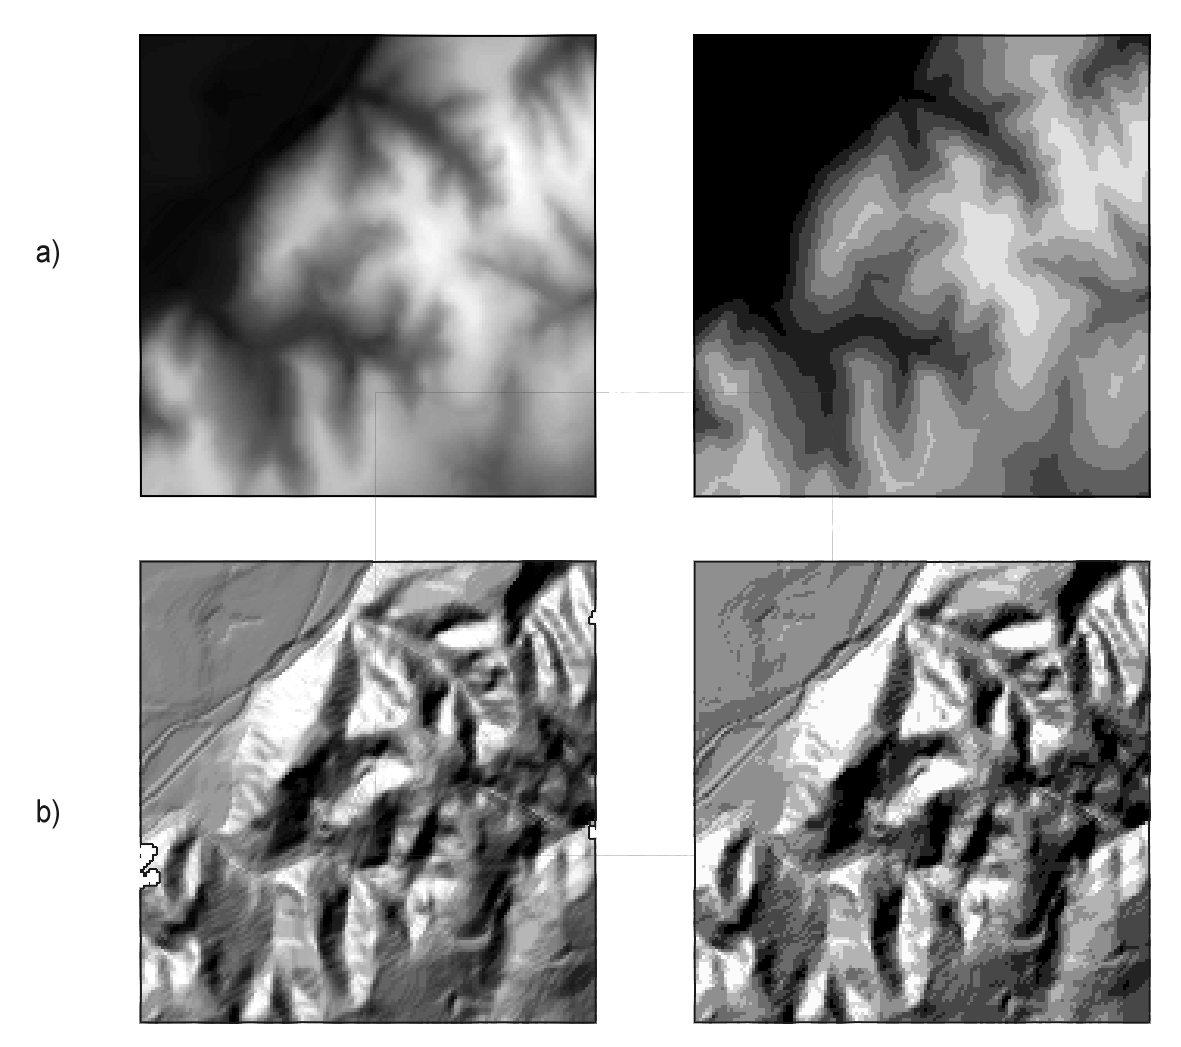
\includegraphics[width=\mycolumnwidth]{Visualizacion_SIG/RepresentacionRaster.png}
\caption{\small Representaci�n de dos capas r�ster con valores de elevaci�n (a) y �ngulo de iluminaci�n (b) mediante 255 (izquierda) y 8 (derecha) clases.}
\label{Fig:RepresentacionRaster} 
\end{figure}

Las representaciones de la parte derecha de la figura, con un total de 255 clases, dan m�s detalle sobre la distribuci�n de la variable a lo largo del mapa que las de la parte izquierda, con 8 clases. Saber en qu� rango de valores se encuentra una zona dada del mapa puede resultar m�s dif�cil e impreciso, pero a cambio tenemos m�s detalle. En un mapa de coropletas, con unidades grandes bien diferenciadas, usar m�s clases no aporta m�s detalle sobre la distribuci�n de la variable, ya que falta esa suavidad en las transiciones entre unidades. En una capa r�ster, por el contrario, la ganancia es notable. 

La segunda representaci�n de la figura, correspondiente a una capa de relieve sombreado, muestra de forma m�s clara lo anterior. El valor recogido en esta capa representa el �ngulo de incidencia de la fuente de iluminaci�n, lo que se traduce en un color m�s claro o m�s oscuro, tal y como corresponder�a a una mayor o menor iluminaci�n sobre el terreno. Mientras que la representaci�n de la izquierda, con m�s clases, tiene un aspecto m�s realista ya que se asemeja a la cantidad de diferentes grados de iluminaci�n que nuestro ojo percibir�a en la realidad, la de la derecha pierde gran parte de su atractivo visual y de su capacidad de hacer patente el relieve (esto es especialmente notable en la zona llana de la parte superior izquierda). En este caso, el uso de un n�mero limitado de clases no es adecuado, ya que el car�cter de esta capa es eminentemente visual, y los valores que puedan contener la celdas no son relevantes, pero s� lo es convertirlos de la forma m�s fiel posible en distintos grados de iluminaci�n.



\section{Combinaci�n de capas}

Argument�bamos en los primeros cap�tulos de este libro, cuando present�bamos el concepto de \emph{capa}, que el verdadero �xito de este concepto es la separaci�n de los distintos tipos de informaci�n geogr�fica, atomizando esta en unidades autocontenidas que guardan tan solo la informaci�n relativa a una variable o fen�meno concreto. As�, cuando adquirimos un mapa impreso, obtenemos muchas variables distintas que no podemos separar, pero en un SIG, y con la informaci�n ya separada en esas capas, la situaci�n es muy distinta, dando lugar a un manejo m�s estructurado y eficaz.

Pese a esto, resulta claro que a la hora de representar la informaci�n geogr�fica, una capa aislada no constituye la forma �ptima de visualizar esta. Si en un mapa encontramos elementos variados, ello no obedece a la mera econom�a de espacio, sino a que a�adir informaci�n adicional a la de esa capa que queremos representar nos ayuda a entenderla mejor. Los procesos que tienen lugar en el espacio est�n relacionados unos con otros, y visualizar esas relaciones aporta una mayor riqueza a la visualizaci�n, haciendo que sea m�s sencillo extraer la informaci�n contenida en ella. Podemos ver un claro ejemplo de esto en la figura \ref{Fig:DiferenciaCombinacionCapas}

\begin{figure}[!hbt]
\centering
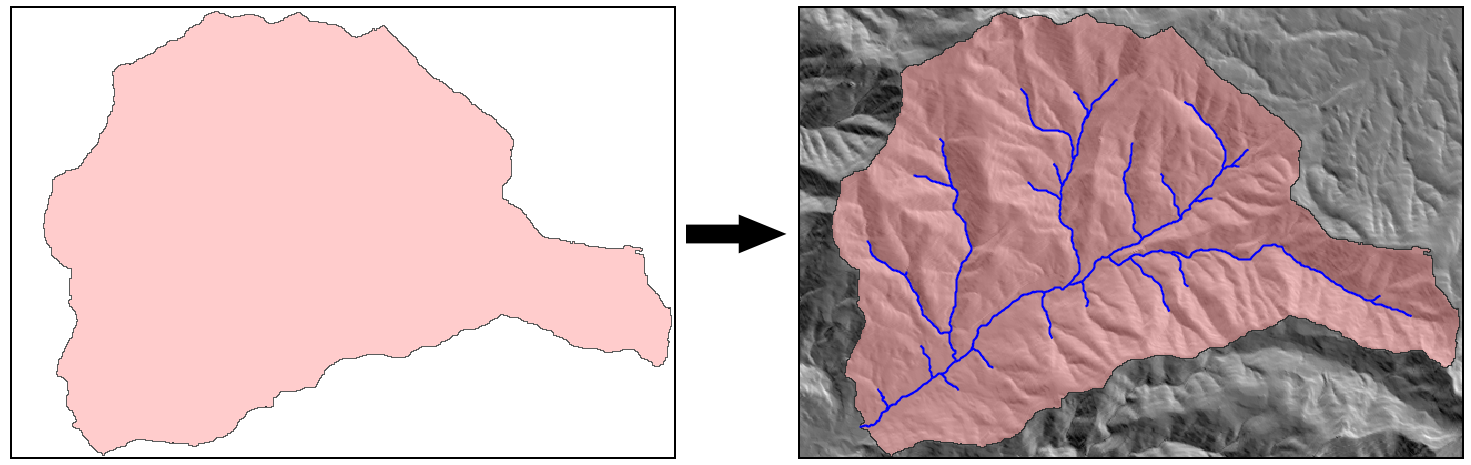
\includegraphics[width=\mycolumnwidth]{Visualizacion_SIG/DiferenciaCombinacionCapas.png}
\caption{\small A�adir capas adicionales que complementen a aquella que resulta de inter�s nos ayuda a interpretar mejor esta y a lograr una representaci�n m�s eficaz.}
\label{Fig:DiferenciaCombinacionCapas} 
\end{figure}

La capa que representa la cuenca vertiente a un punto, y que contiene un solo pol�gono, resulta mucho m�s �til visualmente si la acompa�amos de elementos b�sicos como el relieve y los cauces principales. La imagen de la derecha es autoexplicativa y se ve claramente gracias al relieve que el pol�gono delimita la cuenca. En la de la izquierda esa informaci�n no puede deducirse �nicamente de la capa de inter�s.

Aunque sencillo de llevar a cabo en lo que a manejo del SIG respecta, combinar capas es un proceso que tambi�n debe realizarse con conocimiento y en el que, si se realiza correctamente, las diferencias pueden ser notables. No solo se trata de dar espacio dentro del mapa a toda la informaci�n que esas capas contienen, sino que exista una sinergia entre ellas en la medida de lo posible, para que se complementen mutuamente como partes de un conjunto. Veremos en este apartado algunas ideas a tener en cuenta en este sentido.

El primer aspecto a considerar es el orden de las capas, que indica c�mo se disponen estas las unas sobre las otras y definen el orden de pintado. Si una misma zona est� ocupada por elementos de varias capas, solo ser�n visibles los correspondientes a la capa superior, ya que la representaci�n de los pertenecientes a las dem�s quedar� oculta. El efecto es el mismo que si pint�ramos en un papel algo y encima de ello pint�ramos despu�s algo distinto. Tan solo ver�amos esto �ltimo. 

La figura \ref{Fig:OrdenPintadoCapas} muestra un claro ejemplo de lo anterior en el que se puede apreciar la diferencia que supone variar el orden de las capas.

\begin{figure}
\centering
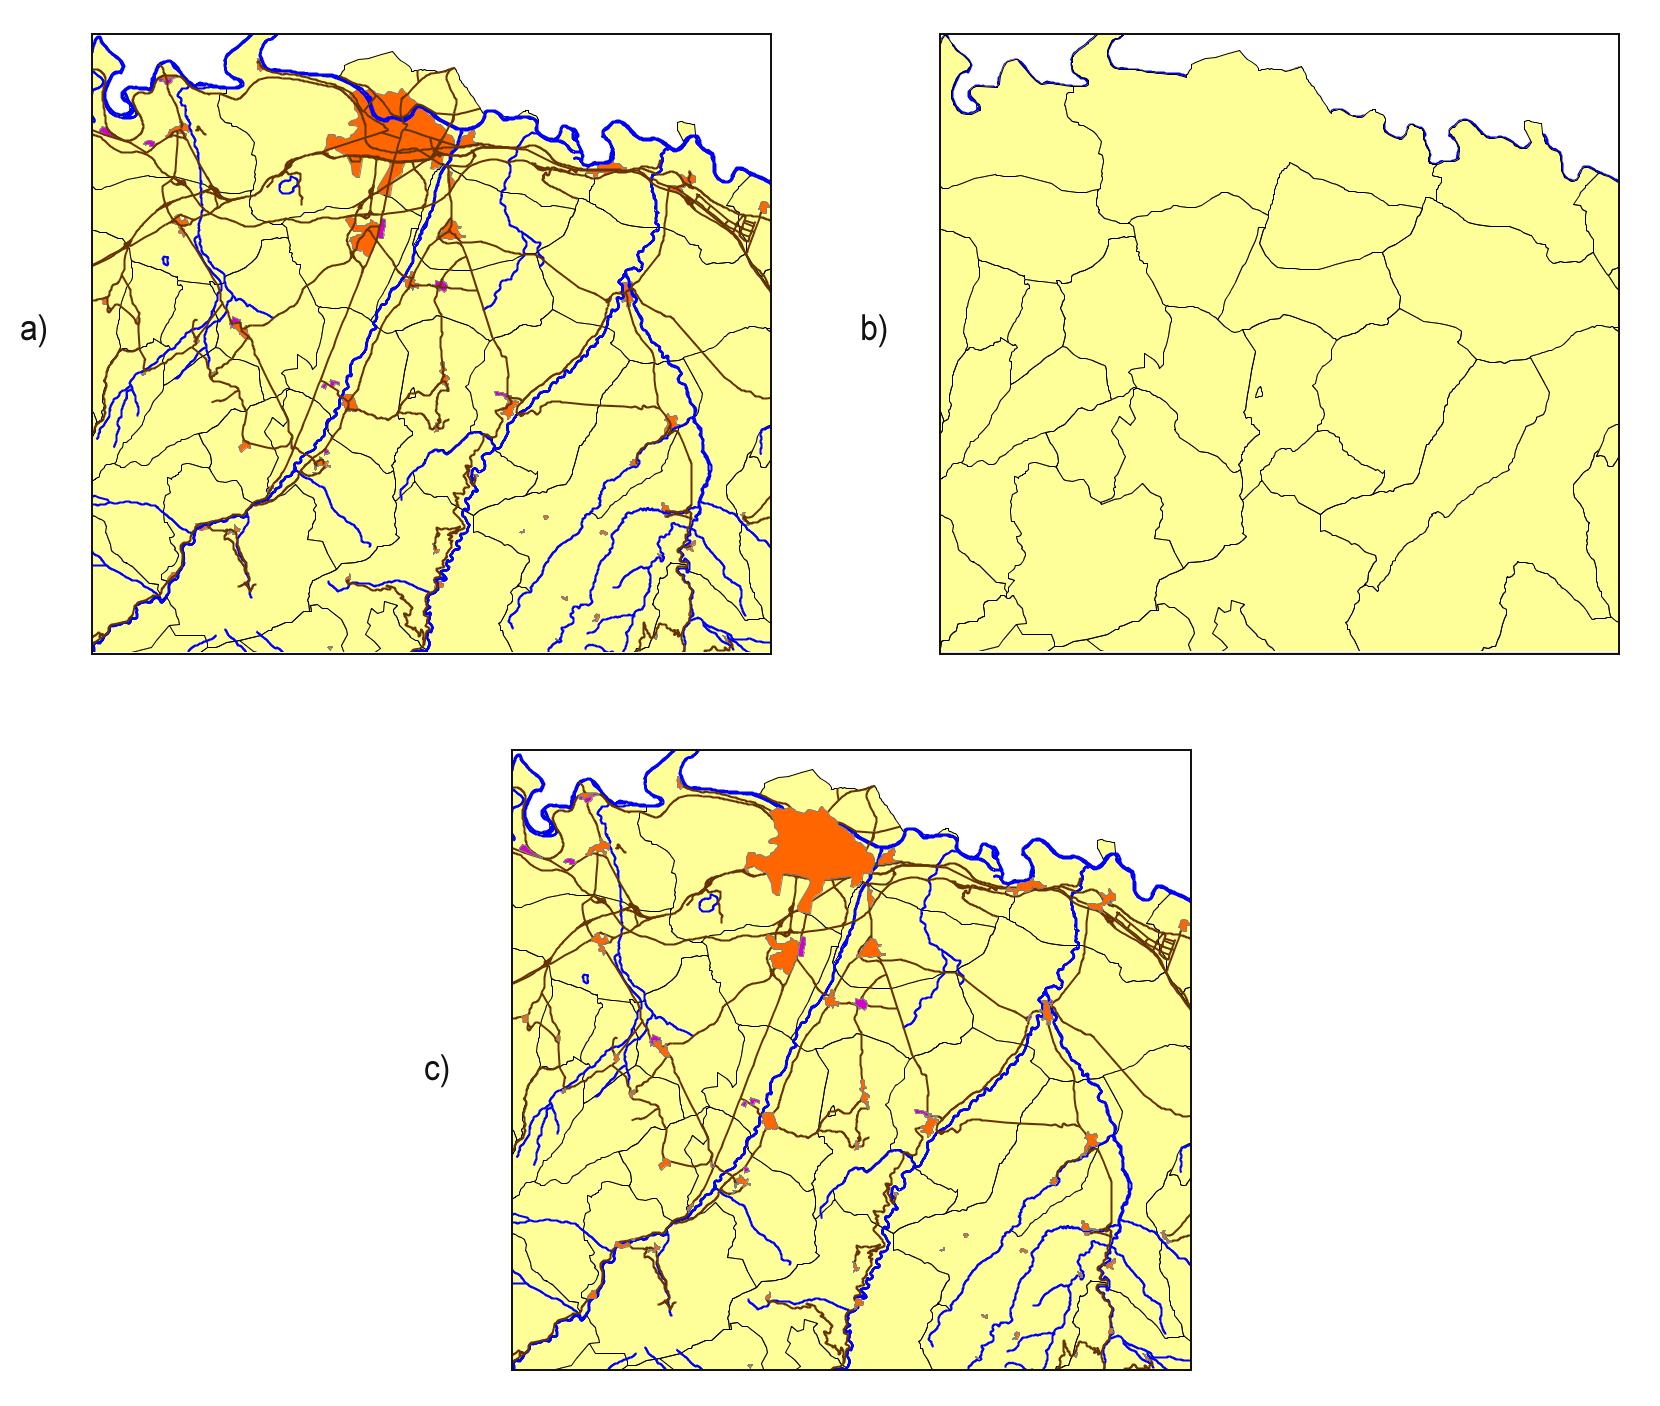
\includegraphics[width=\mycolumnwidth]{Visualizacion_SIG/OrdenPintadoCapas.png}
\caption{\small Variar el orden de las capas puede suponer un cambio radical en la representaci�n final obtenida. Todas las im�genes proceden del mismo conjunto de capas, pero las representaciones son muy distintas.}
\label{Fig:OrdenPintadoCapas} 
\end{figure}

A pesar de estar construidas a partir de las mismas capas, las representaciones mostradas en la figura son muy distintas como documentos cartogr�ficos y no proporcionan la misma informaci�n. As�, en el caso b), pr�cticamente toda la informaci�n esta <<oculta>>, ya que hay una capa que la cubre. En el caso c) sucede que las zonas urbanas (en marr�n) est�n situadas por encima de las capas de r�os y v�as de comunicaci�n, dando la sensaci�n de que estas �ltimas desaparecen al entrar en dichas �reas urbanas. Este puede ser un efecto deseado en ciertos casos, para enfatizar las zonas urbanas y su contorno, pero la representaci�n es menos informativa en caso de que quiera detallarse el trazado de cauces y carreteras.

Se ve claramente que el orden de pintado es importante, y que un correcto orden es vital para acomodar todos los elementos a representar y que cada uno cumpla su labor como elemento informativo.

Sabemos que las capas r�ster llenan todo el espacio y contienen valores en todas sus celdas (o p�xeles en el caso de im�genes). Por ello, van a tapar lo que se sit�e por debajo de ellas y no resulta buena idea situarlas en lo alto del orden de pintado. En su lugar, se deben considerar como capas base sobre las que situar las restantes, de tal modo que no impidan a estas visualizarse correctamente.

Con un razonamiento similar, podemos establecer la mejor forma de ordenar las capas vectoriales, situando por norma general los pol�gonos y encima de estos las l�neas y los puntos respectivamente. Esta regla es, l�gicamente, muy gen�rica, y en cada situaci�n se ha de evaluar la conveniencia de adoptar otra disposici�n, siempre con objeto de evitar que unas capas dificulten la correcta interpretaci�n de otras.

En ocasiones, un determinado orden viene impuesto por el significado que tienen las capas. Por ejemplo, si nuestro mapa contiene una capa con la red de drenaje y otra con carreteras, lo l�gico y habitual es que las carreteras est�n por encima de los r�os, ya que lo normal es que pasen por encima de estos y no al contrario. En la practica cartogr�fica, este tipo de situaci�n se resuelve simbolizando de forma particular este tipo de coincidencias, como se muestra en la figura \ref{Fig:CruceCarreterasRios}. Esto requiere en el SIG unas capacidades avanzadas de edici�n gr�fica, algo que, como vimos en el primer cap�tulo de esta parte, no es muy com�n. No obstante, algunos SIG incluyen no solo esas capacidades, sino tambi�n funcionalidades que crean autom�ticamente esos elementos gr�ficos en funci�n del an�lisis de las capas, de tal modo que automatizan la tarea.

\begin{figure}[!hbt]
\centering
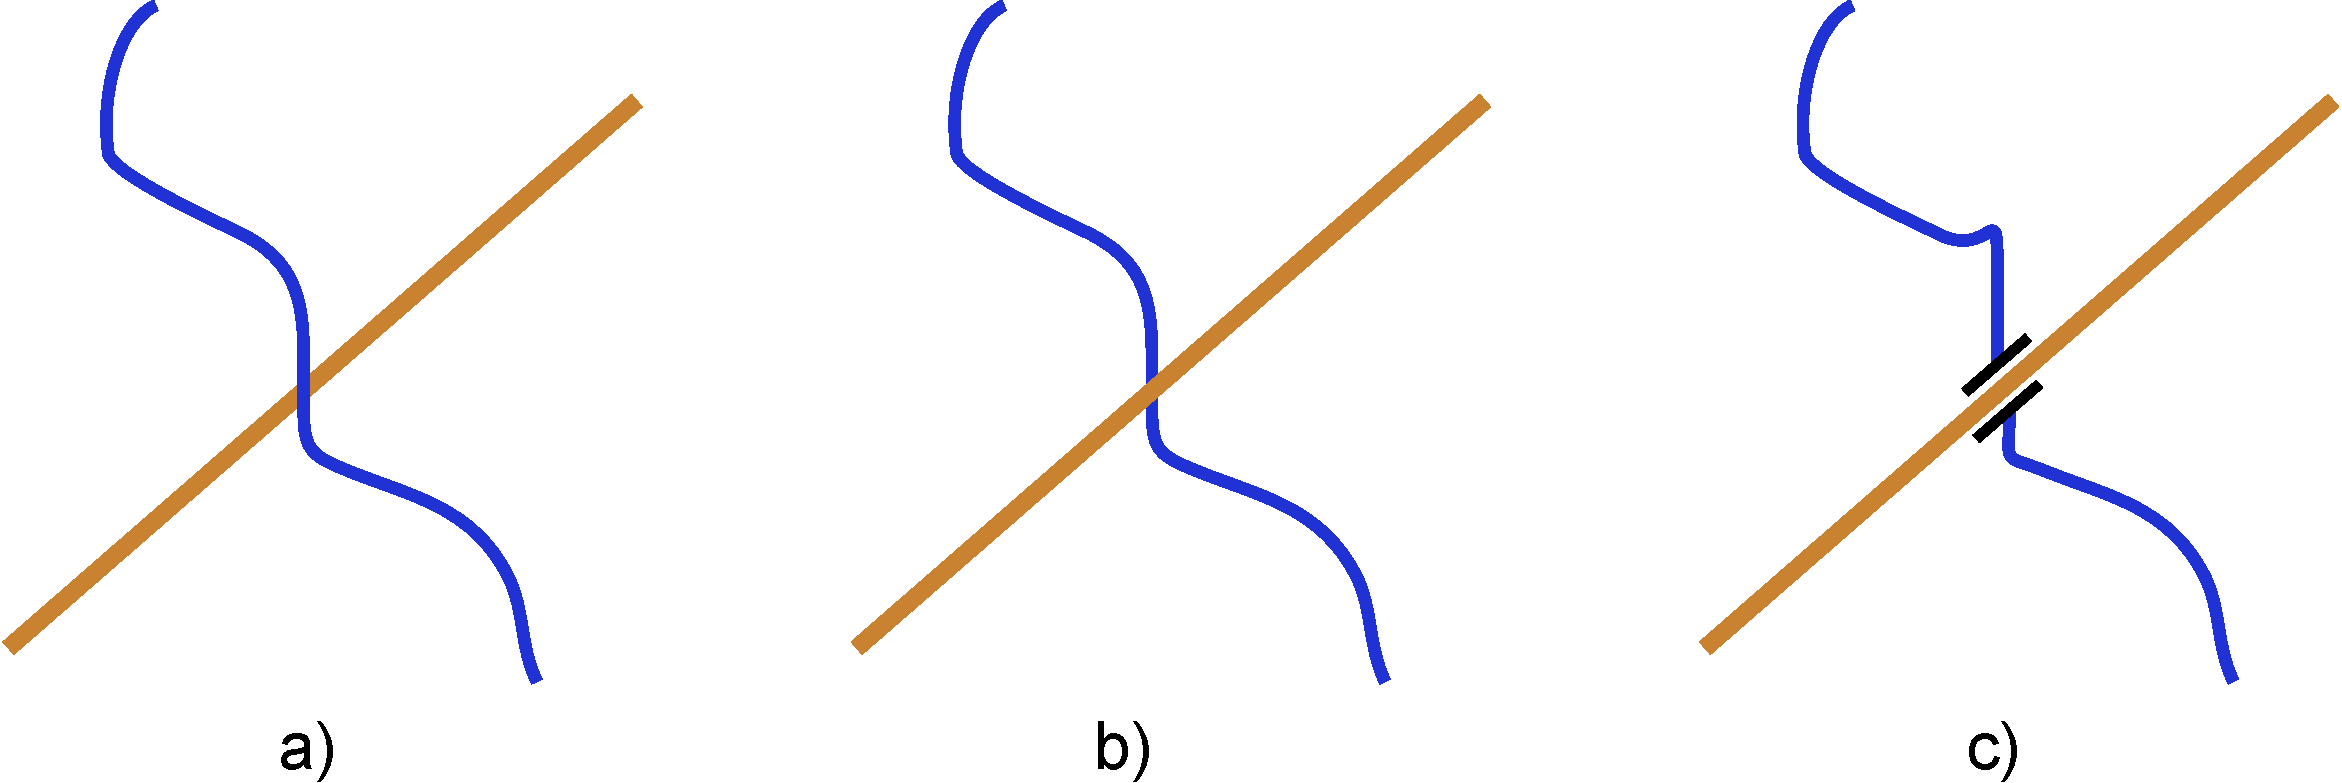
\includegraphics[width=0.7\mycolumnwidth]{Visualizacion_SIG/CruceCarreterasRios.pdf}
\caption{\small Representaci�n erronea (a) y correcta (b) de capas al combinar una de carreteras (en marr�n) y otra de red de drenaje (en azul). La inclusi�n de un elemento que simbolice el cruce (c) supone, no obstante, una mejor soluci�n desde el punto de vista cartogr�fico.}
\label{Fig:CruceCarreterasRios} 
\end{figure}


Una funcionalidad de que disponen los SIG para la combinaci�n de capas es el uso de transparencias y semi--transparencias. Estas se pueden aplicar tanto a capas r�ster como vectoriales, de forma que puede verse a trav�s de ellas y as� presentar la informaci�n de otras capas que se encuentren por debajo. Por ejemplo, la representaci�n mostrada en la figura \ref{Fig:DiferenciaCombinacionCapas} hace uso de esta t�cnica. El pol�gono que delimita la cuenca vertiente es semi-transparente, de tal modo que la capa de relieve sombreado que est� debajo puede verse, dando la sensaci�n de que sigue ese relieve.

Si se usa semi--transparencia para una capa tem�tica (por ejemplo, en un mapa de coropletas), no debe perderse de vista que el color var�a respecto al original que ha sido asignado a cada pol�gono, ya que se <<mezcla>> con el color de cada p�xel correspondiente a la representaci�n de las capas inferiores. Esto puede resultar confuso a la hora de interpretar las componentes del color, ya que no coincidir�n con las mostrada en la leyenda. M�s a�n, y como puede tambi�n apreciarse en la figura \ref{Fig:DiferenciaCombinacionCapas}, el color del pol�gono, que deber�a ser �nico, no lo es, ya que la parte que se transparenta a trav�s de este no es uniforme. En el caso mostrado en la figura, este hecho no tiene importancia, pero debe considerarse al representar otro tipo de variables en las que el color tiene un significado definido, para garantizar que ese significado se transmite de igual modo.

En el caso de una capa r�ster, puede aplicarse una transparencia total, haciendo que determinadas partes de esta no se representen. A pesar de que la capa r�ster contiene informaci�n en todas las celdas de su extensi�n, no todas se representan. Esto es especialmente �til para capas de tipo categ�rico. La figura \ref{Fig:Zona_influencia_vehiculo} es un buen ejemplo de esto. En ella, la capa que contiene el �rea de influencia es una capa r�ster, ya que ha sido creada mediante un an�lisis r�ster (repasa el apartado para ver c�mo se ha calculado, si no lo recuerdas). Sin embargo, se puede combinar con la capa de pendientes, ya que solo se pintan las celdas correspondientes a dicho �rea de influencia pero no las restantes. Para llevar esto a cabo se suele asignar la transparencia a un valor o serie de valores definidos, habitualmente al valor que codifica la ausencia de datos (que en este caso es el empleado para codificar aquellas celdas que no forman parte del �rea de influencia calculada).

El uso de transparencia sirve tambi�n para combinar im�genes que se solapan y eliminar las partes de estas que no contienen informaci�n. Como vimos en la secci�n \ref{Modelo_raster}, la forma de la imagen es siempre rectangular y tiene una orientaci�n fija. Esto no ha de coincidir obligatoriamente con la informaci�n que contiene, siendo necesario en ese caso rellenar las �reas sin informaci�n con alg�n tipo de valor. A la hora de combinar capas, esos valores de relleno no interesa representarlos.

%La figura \ref{Fig:CombinacionCapasTransparencia} muestra un caso en el que se dispone de dos im�genes de una zona en la frontera entre dos regiones administrativas. Cada una de las im�genes ha sido obtenida de la administraci�n correspondiente, que solo provee los datos relativos a su territorio, motivo por el cual ambas im�genes contienen zonas en negro. Mediante el uso de transparencia pueden combinarse sin que esas zonas negras se visualicen, logrando una representaci�n uniforme (considerando, obviamente, que las im�genes han sido tomadas en condiciones distintas y por ello existen diferencias de tonalidad e iluminaci�n, entre otras).
%
%\begin{figure}[!hbt]
%\centering
%\includegraphics[width=0.8\mycolumnwidth]{Visualizacion_SIG/CombinacionCapasTransparencia.png}
%\caption{\small Combinaci�n de im�genes incompletas mediante uso de transparencias en zonas sin datos.}
%\label{Fig:DiferenciaCombinacionCapas} 
%\end{figure}

La divisi�n horizontal de los datos puede dar lugar a problemas en el caso de capas vectoriales o capas r�ster distintas de im�genes, para las que es necesario establecer unas caracter�sticas de representaci�n en funci�n de sus atributos, en caso de que la informaci�n acerca de una variable se encuentre dividida en varias capas, cada una de las cuales cubre una porci�n del terreno. Un SIG incorpora habitualmente herramientas para que estas capas, as� divididas para una mejor gesti�n, puedan unirse en una �nica, y al hacer esto, la capa resultante tendr� asignado un esquema de representaci�n tambi�n �nico, de forma que toda ella se visualizar� de forma coherente. En tal caso, no encontramos problema alguno.

En el caso, sin embargo, de trabajar con las capas de forma independiente, y si estas han de combinarse en una misma representaci�n, es necesario que los esquemas de representaci�n sean coherentes unos con otros, para que en la representaci�n global aparezcan como una �nica capa de informaci�n. De modo contrario, la representaci�n ser� ambigua y confusa, y no mostrar� de la forma adecuada la informaci�n que esas capas contienen. No considerar esta circunstancia lleva a errores tales como los mostrados en la figura \ref{Fig:Representacion_capas_incoherente}. 


\begin{figure}[!hbt]
\centering
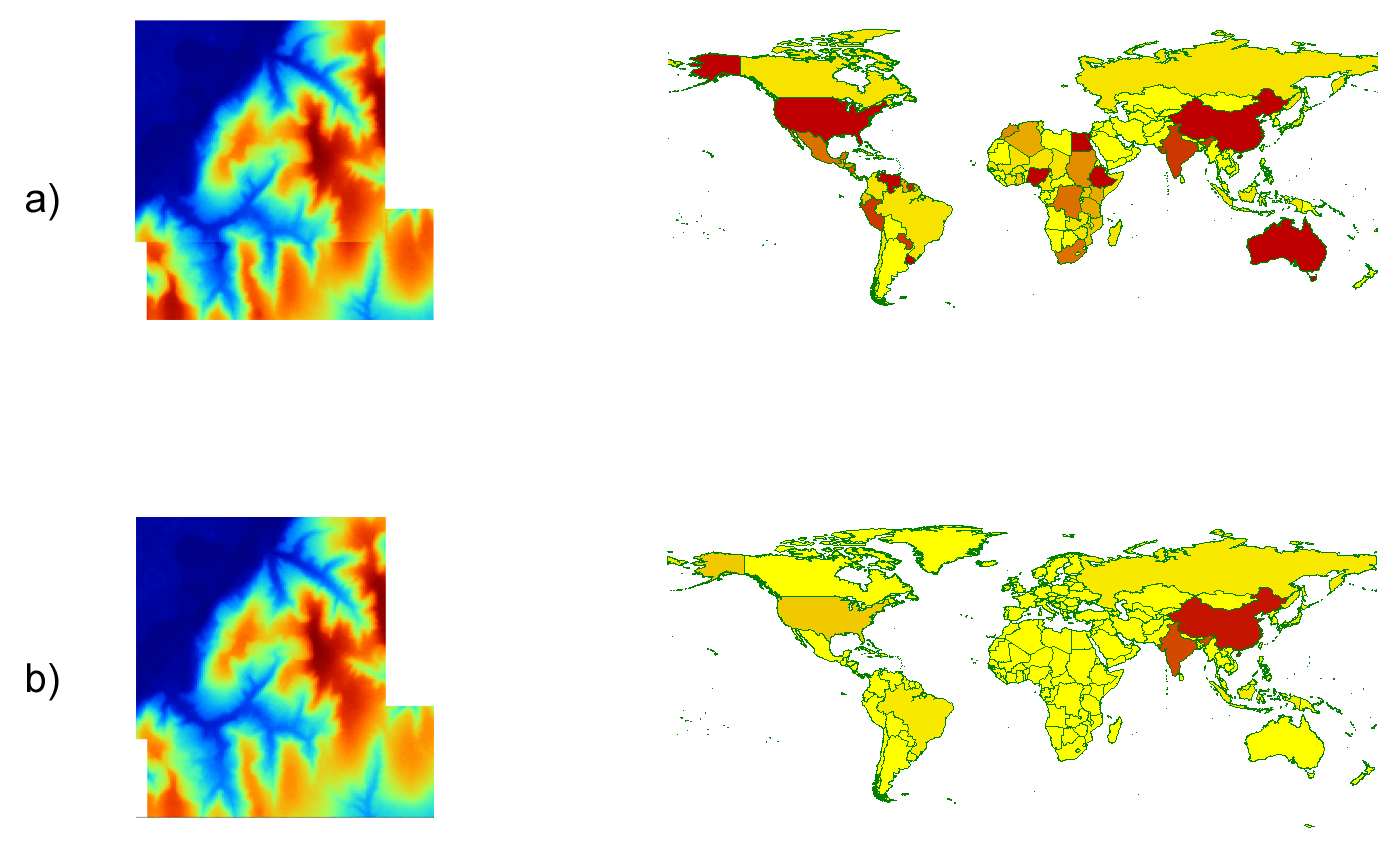
\includegraphics[width=.9\textwidth]{Visualizacion_SIG/Representacion_capas_incoherente.png}
\caption{\small a) dos representaciones incorrectas de conjuntos de capas, debido a incoherencia entre los par�metros de representaci�n empleados en cada una de ellas. b) representaci�n correcta y homog�nea con par�metros de representaci�n comunes.}
\label{Fig:Representacion_capas_incoherente} 
\end{figure}

En el caso de la derecha, dos MDE se representan con una misma gradaci�n de colores. Se usa una representaci�n por intervalos, pero, debido a que los valores extremos a partir de los cuales se crean dichos intervalos son distintos, estos intervalos resultan tambi�n distintos, y un mismo color representa un valor de elevaci�n diferente en cada capa. Por esta raz�n, se hace muy patente la l�nea de uni�n entre ambas capas, ya que, pese a que existe una continuidad suave entre los valores, no lo es as� en lo que respecta a su representaci�n.

El mismo par de capas puede representarse de forma correcta sin m�s que establecer un �nico conjunto de intervalos para ambas, de tal modo que los valores m�ximos y m�nimos entre los que se sit�en sean los m�ximos y m�nimos absolutos del conjunto de capas.

En el caso de la izquierda (que ya se describi� en el apartado \ref{Juntar_capas} dedicado a la operaci�n de juntar capas vectoriales) se presenta el mismo error, aunque no resulta tan patente a primera vista como en el anterior. La representaci�n esta realizada a partir de cinco capas de datos, una para cada continente, asignando colores en funci�n de la poblaci�n de cada pa�s y con un total de 10 intervalos. Aunque la representaci�n no revela ning�n problema tal como la l�nea de sutura entre las capas r�ster del ejemplo a), es incorrecta, ya que pa�ses con poblaciones muy distintas se representan con un mismo color. As�, Alemania, el pa�s m�s poblado del contiene europeo, y China, el m�s poblado de Asia, tienen el mismo color a pesar de este �ltimo tiene m�s de quince veces m�s habitantes que el primero. Una vez m�s, los intervalos empleados no son coherentes entre s�. En la representaci�n de la derecha de la figura puede observarse el resultado tras haber ajustado convenientemente los par�metros de representaci�n del conjunto de capas. N�tese que, pese a ser correcto desde este punto de vista, el mapa es poco informativo. La divisi�n en intervalos iguales que se ha empleado no resulta una buena opci�n en este caso debido a la presencia de unos pocos pa�ses con mucha m�s poblaci�n que el resto. El uso de intervalos naturales o percentiles habr�a dado lugar a una representaci�n m�s �til.

\section{Particularidades de la representaci�n en pantalla}

Tanto para las representaciones en papel como para las representaciones en pantalla se siguen unos mismos principios a la hora de dise�arlas, pero estas �ltimas presentan algunas caracter�sticas particulares que hacen necesario tener en consideraci�n otros factores. Esto es especialmente cierto cuando consideramos que esa representaci�n en pantalla se realiza desde dentro de un SIG como parte de una sesi�n de trabajo con este (es decir, que no estamos, por ejemplo, visualizando un mapa escaneado con una aplicaci�n de edici�n de im�genes sino trabajando en el SIG y creando la visualizaci�n como un elemento m�s de ese trabajo).

Podemos distinguir dos bloques fundamentales de diferencias que hacen que un mapa pensado para ser visualizado en la pantalla mientras ejecutamos un SIG no deba dise�arse exactamente igual que si estuviera pensado exclusivamente para ser utilizado en un soporte impreso: la baja resoluci�n de la pantalla y la interactividad de la propia representaci�n.

El primer aspecto a considerar es la baja resoluci�n de una pantalla en comparaci�n con un documento impreso. Mientras que sobre el papel un mapa puede imprimirse a una resoluci�n de varios cientos de puntos por pulgada (dpi), en la pantalla la resoluci�n viene limitada por el tama�o de los p�xeles, que es mucho mayor que el del m�nimo punto que se consigue imprimir por medios mec�nicos. En una pantalla, la resoluci�n es del orden de 100 p�xeles por pulgada. Por eso, si te acercas a la pantalla de tu ordenador, puedes ver los p�xeles individuales si tienes cierta agudeza visual. Por el contrario, incluso con una impresora de uso dom�stico, distinguir el m�nimo punto que esta es capaz de imprimir est� por encima de la capacidad del ojo humano. Esto quiere decir que el papel permite una definici�n mucho mayor que la pantalla, ya que incluso los elementos de menor tama�o del mapa van a estar dibujados con una serie puntos de menor tama�o que permiten lograr una nitidez muy elevada. \index{Dots per inch (dpi)}\index{Puntos!por pulgada|see{Dots per inch (dpi)}}

A la hora de preparar cartograf�a impresa, la resoluci�n no es un problema, ya que las capacidades de que se dispone superan a las necesidades que el cart�grafo puede tener. En la pantalla, sin embargo, algunos elementos pueden no aparecer con suficiente claridad y, aunque en papel cumplan su funci�n correctamente, es conveniente sustituirlos por otros m�s adecuados cuando no se trabaja sobre un medio impreso. Los siguientes son algunos de los elementos que deben evitarse o, al menos, emplearse de manera distinta a la hora de crear representaciones en pantalla.

\begin{itemize}
	\item Fuentes con ornamentos tales como sombreados. Si son de peque�o tama�o, el sombreado no puede pintarse con suficiente nitidez y perjudica la legibilidad del texto.
	\item Fuentes con \emph{serifas}. Las serifas (Figura \ref{Fig:Serifas}) est�n pensadas para hacer m�s c�moda la lectura del texto impreso cuando este tiene una longitud considerable tal como en un libro, y consisten en peque�os adornos generalmente situados al final de las l�neas. Por su peque�o tama�o, no se representan con suficiente definici�n en la pantalla, lo que causa p�rdida de legibilidad. Por ello, se recomienda el uso de fuentes sin serifas en documentos pensados para visualizarse en pantalla, tales como paginas Web o como un mapa dentro de un SIG.\index{Serifa}
	\item Rellenos con tramas de paso muy fino. Si las l�neas de un tramado est�n muy juntas, la baja resoluci�n de la pantalla puede ser insuficiente para separarlas, haciendo dif�cil para el observador reconocerlas.
	\item Punteados. Al igual que en el caso anterior, si el punteado no tiene un paso suficiente, puede no resultar evidente la discontinuidad de la linea, cre�ndose una representaci�n ambigua.
\end{itemize}

\begin{figure}[!hbt]
\centering

\includegraphics[width=0.35\mycolumnwidth]{Visualizacion_SIG/Serifas.png}
\caption{\small Concepto de serifa.}
\label{Fig:Serifas} 
\end{figure}

El segundo aspecto a considerar es el relativo a la interactividad de las representaciones. A diferencia de un mapa impreso, en un SIG lo que vemos no es un elemento est�tico, sino din�mico. En este contexto, \emph{din�mico} no quiere decir que el mapa cambie o que represente un proceso din�mico (que tambi�n es posible, como veremos m�s adelante en otro apartado de este cap�tulo), sino que el usuario puede alterarlo utilizando por lo menos las herramientas m�s fundamentales que proporcionan interactividad, tales como el desplazamiento, el acercamiento o el alejamiento, seg�n ya vimos en el apartado \ref{Funcion_SIG_Visualizacion}. Este hecho hace que aparezcan algunos problemas, entre los que destacan los relacionados con el rendimiento y aquellos que derivan de la posibilidad de variar sensiblemente la escala de representaci�n.

Respecto al rendimiento, no debe olvidarse que cada vez que formamos la imagen de un mapa en la pantalla (algo que sucede cada vez que ajustamos el encuadre mediante esas herramientas interactivas), el SIG ha de realizar un gran n�mero de c�lculos correspondientes a operaciones como las siguientes:

\begin{itemize}
	\item Remuestreo de las im�genes.
	\item Asignaci�n de colores o patrones a los distintos elementos (geometr�as en capas vectoriales o celdas en capas r�ster) en funci�n de los valores asociados a estos.
	\item Dibujado de geometr�as.
\end{itemize}

En funci�n de la complejidad y el tama�o de las capas que estemos representando, as� como del n�mero de estas, generar esa representaci�n puede suponer un volumen muy elevado de operaciones, lo cual har� poco fluido el trabajo en el SIG, llegando incluso a hacer inoperativa la propia interactividad del programa en un caso extremo. Cuando esto sucede, es necesario sacrificar algo de precisi�n y rigor cartogr�fico en beneficio del rendimiento, especialmente cuando la falta de rendimiento y la lentitud del sistema nos dificulten la realizaci�n de otras operaciones tales como, por ejemplo, el an�lisis de esas mismas capas que representamos, o incluso la propia navegaci�n.

Trabajar con capas de menor detalle ---por ejemplo, capas r�ster de menor resoluci�n o capas vectoriales con l�neas simplificadas (v�ase \ref{Generalizacion_lineas})--- es una soluci�n a este problema, aunque no necesariamente excluye la posibilidad de trabajar con las capas originales. Un planteamiento multi--escalar en el que, seg�n la escala, se visualicen unas u otras capas, es una soluci�n frecuente a esta problem�tica. Vimos estas ideas en el apartado \ref{Generalizacion_en_SIG}, donde presentamos el concepto de \emph{pir�mide} como recurso empleado en estos casos para el trabajo con capas r�ster.\index{Pir�mides}

Tambi�n se puede aumentar la velocidad de dibujado utilizando colores lisos en lugar de tramas, y evitando los textos de gran tama�o o los s�mbolos complejos que provengan de im�genes muy detalladas y de gran tama�o.

Por �ltimo, el hecho de que la escala de la representaci�n pueda variar seg�n la voluntad del usuario puede causar problemas con algunos de sus elementos  tales como s�mbolos o etiquetas de texto. Si todos los elementos del mapa se escalan proporcionalmente, una reducci�n importante de escala disminuir� el tama�o del texto hasta hacerlo ilegible. Por el contrario, si aumentamos la escala el tama�o puede ser excesivo. La figura \ref{Fig:ProblemasRepresentacionSimbolos} muestra este hecho. 

El mismo problema sucede en el caso de emplear s�mbolos. Si, por ejemplo, tenemos una capa de puntos con la localizaci�n de bocas de incendios y representamos cada uno con un peque�o dibujo de una de ellas, al aumentar el tama�o de cada icono se perder� definici�n, mientras que al disminuirlo la pantalla no tiene resoluci�n suficiente para dibujarlo correctamente y no se identificar� su forma. En general, el empleo de s�mbolos puntuales de este tipo se desaconseja a la hora de representar cartograf�a en pantalla.


\begin{figure}[!hbt]
\centering
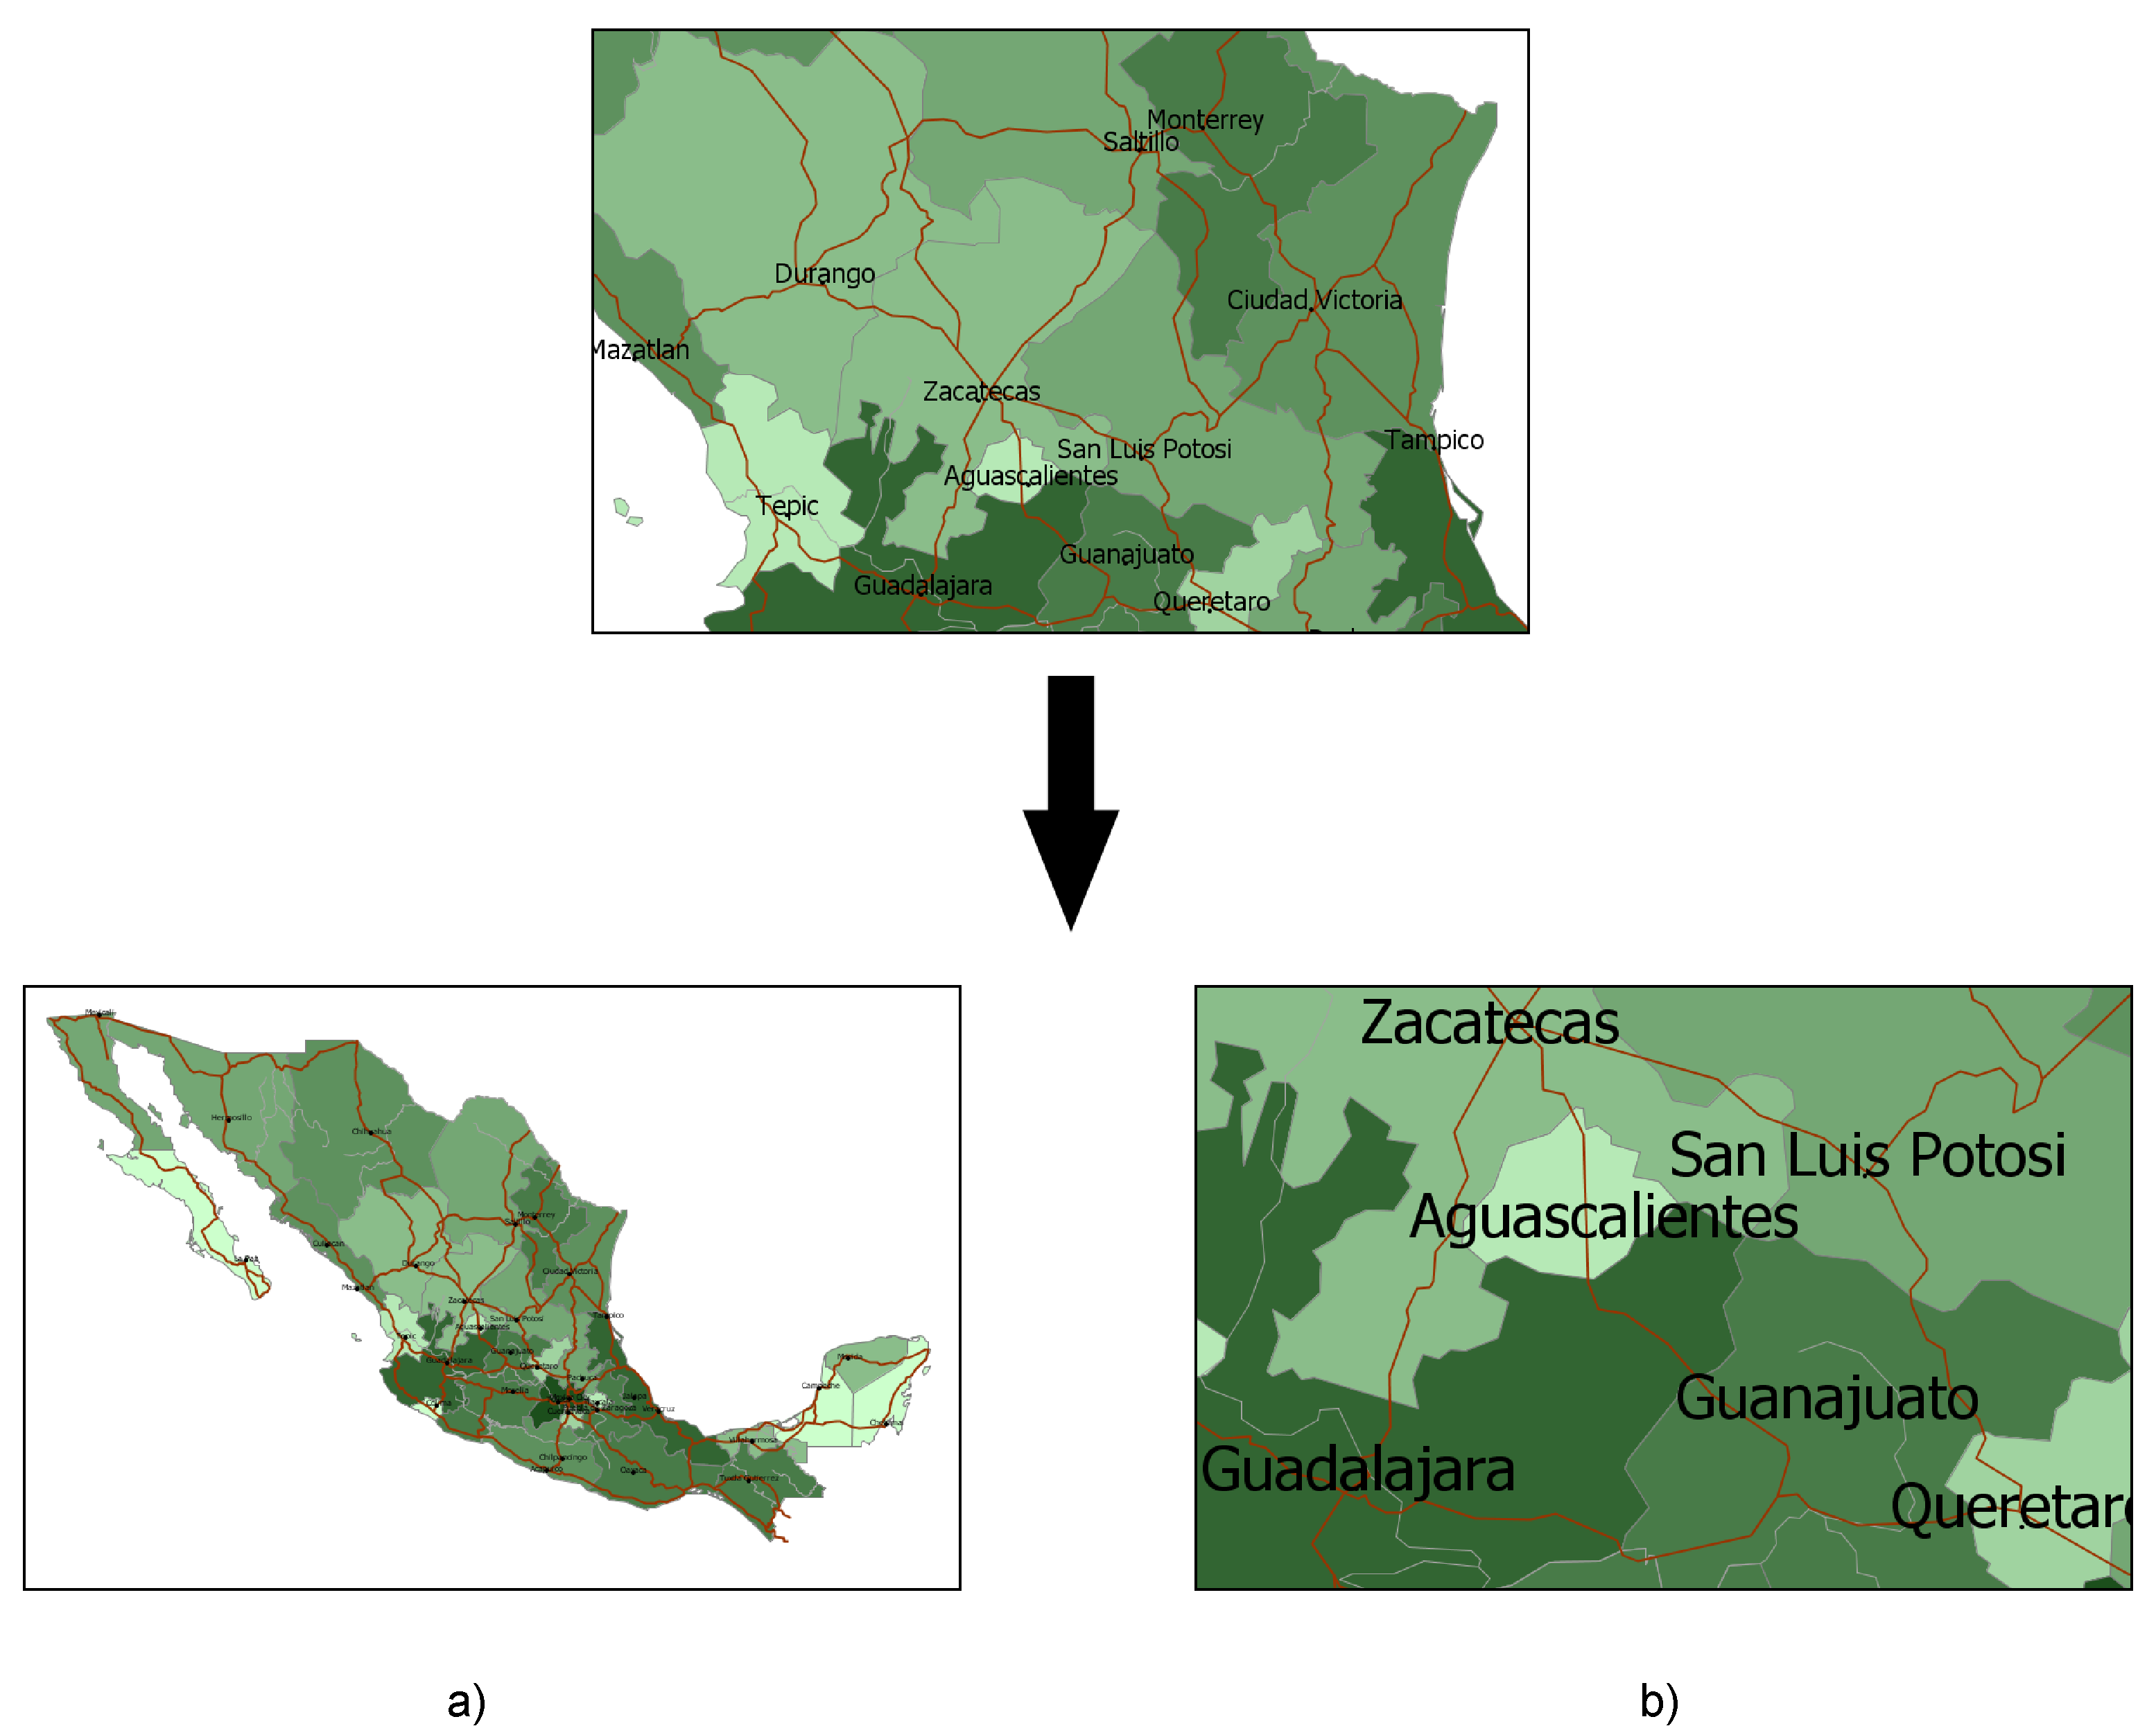
\includegraphics[width=0.85\mycolumnwidth]{Visualizacion_SIG/ProblemasRepresentacionSimbolos.pdf}
\caption{\small El cambio de escala var�a el tama�o de los s�mbolos tales como las etiquetas, haci�ndolos demasiado peque�os (a) o demasiado grandes (b)}
\label{Fig:ProblemasRepresentacionSimbolos} 
\end{figure}


Una soluci�n a esto es especificar un tama�o absoluto de estos elementos que no var�e con la escala. Es decir, que un s�mbolo o una etiqueta de texto tengan siempre el mismo tama�o en pantalla y ocupen los mismos p�xeles. A escalas bajas, sin embargo, este m�todo puede dar lugar a representaciones saturadas, como se observa en la figura \ref{Fig:RepresentacionSaturada}. Este problema es m�s notable si se tiene en cuenta que en pantalla se emplean generalmente tama�os de letra m�s grandes que en un mapa impreso, por lo que se debe reducir la cantidad de texto mostrado para evitar una densidad de etiquetas demasiado elevada.


\begin{figure}[!hbt]
\centering
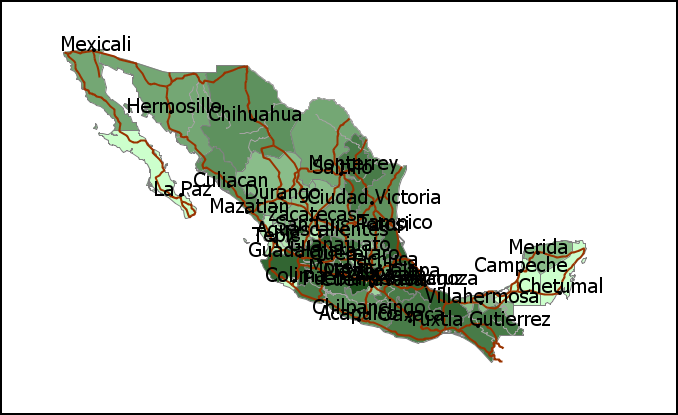
\includegraphics[width=0.7\mycolumnwidth]{Visualizacion_SIG/RepresentacionSaturada.png}
\caption{\small Representaci�n saturada al representar elementos con tama�o fijo a una escala baja.}
\label{Fig:RepresentacionSaturada} 
\end{figure}

Las particularidades que hemos visto en esta secci�n se refieren a la representaci�n en la pantalla de un ordenador de sobremesa o port�til, pero, como vimos en el cap�tulo \ref{SIG_Moviles}, los SIG sobre dispositivos m�viles tienen a su vez sus propias caracter�sticas en lo que a dispositivos de representaci�n respecta. Por ello, y seg�n los casos, todo lo visto en este apartado debe considerarse de modo espec�fico en estos casos, a�adiendo los condicionantes que este hecho puede implicar en las distintas funciones de representaci�n.


\section{Visualizaci�n tridimensional}

La visualizaci�n tridimensional es una de las tendencias m�s importantes dentro del �mbito SIG en la actualidad. Aunque el SIG de escritorio sigue siendo fundamentalmente una herramienta 2D, las aplicaciones con capacidades 3D van ganando relevancia al tiempo que incorporan cada vez m�s funcionalidades que las acercan a las del SIG de escritorio completo. Adem�s de su mejor capacidad para incorporar de forma realista los elementos geogr�ficos (que son tridimensionales, as� como los fen�menos que los originan), una de las razones indudables del �xito y la popularidad del SIG 3D es su gran atractivo visual. La tercera dimensi�n hace m�s sencillo interpretar buena parte de la informaci�n representada, ya que permite mostrarla de un modo m�s asequible y f�cil de entender, especialmente para el observador no especializado. Frente al mapa impreso o la representaci�n bidimensional en pantalla, la representaci�n en tres dimensiones resulta mucho m�s intuitiva y <<real>>. Al ser m�s natural y cercano a la realidad que se representa, un mapa tridimensional se percibe menos como un elemento simb�lico y m�s como una realidad.

Por todo ello, porque el factor visual es de gran relevancia en los SIG 3D, una adecuada visualizaci�n de la informaci�n geogr�fica tiene mucha importancia para poder aprovechar al m�ximo todas sus posibilidades. Las siguientes son algunas de las ideas que deben considerarse al trabajar con representaciones tridimensionales, junto, por supuesto, todas las que ya hemos detallado para las representaciones 2D habituales:

\begin{itemize}	
	\item Existencia de distintas formas de perspectiva. Existen distintas formas de perspectiva para lograr trasladar la realidad tridimensional a la superficie plana del papel o la pantalla. Estas alteran la percepci�n de las distintos elementos de la imagen, y en algunas aplicaciones es posible escoger la que se desea, con lo cual aparece un nuevo par�metro que modifica la representaci�n y debe ser ajustado convenientemente.
	
	\item Importancia de la posici�n del observador y los �ngulos de visi�n. En un mapa plano no existe como tal el concepto de posici�n del observador. Aumentando o disminuyendo la escala, el efecto producido es similar a alejarse o acercarse al mapa, y al desplazar este y cambiar el encuadre, podemos considerar que el observador se desplaza, pero estos movimientos no afectan a c�mo percibimos la informaci�n del mapa. Desde la vista cenital que representa un mapa, apreciamos sin dificultad las dos dimensiones que este contiene, y ello nos permite interpretar el significado de sus distintos elementos. En el caso tridimensional, la posici�n del observador no viene �nicamente definida por una posici�n y un alejamiento (que resultan en un encuadre y una escala dadas), sino por una serie de �ngulos que al modificarse alteran la visi�n de las variables representadas.
	
	Por ejemplo, para el caso de que existan elementos tridimensionales tales como edificios, una vista de tipo cenital no dejar� percibir adecuadamente la elevaci�n de estos. Por el contrario, una capa r�ster de temperaturas representada dentro de esa vista tridimensional sobre el terreno se apreciar� mejor si nos situamos por encima de ella, de forma que la l�nea de visi�n sea perpendicular. 
	
	En otros casos, para una �nica variable es necesario elegir la visualizaci�n en funci�n de aquello que queramos mostrar de forma m�s clara. Si consideramos una capa de l�neas (tridimensional, es decir, formada por un conjunto de puntos definidos mediante 3 coordenadas cada uno) que representa la trayectoria de un avi�n, la vista cenital nos permitir� ver el recorrido de este, pero ser� dif�cil apreciar si ha ascendido o descendido durante el vuelo. Una vista de perfil soluciona esto, pero hace complicado apreciar el desplazamiento en el eje perpendicular a la linea de visi�n, por lo que el recorrido no se conoce con la misma exactitud. Incluso si este puede apreciarse de alg�n modo (por ejemplo, variando el grosor de la l�nea cuando el avi�n se acerca o aleja del observador para as� representar la distancia en profundidad), una capa base con un mapa topogr�fico no se visualizar�a apenas desde esa vista de perfil, haciendo imposible saber cu�ndo en ese recorrido se ha pasado de un pa�s a otro.	A diferencia de lo que sucede con un mapa bidimensional, en una vista tridimensional no se aprecian de igual modo todas las dimensiones implicadas en la representaci�n, ya que el soporte (la pantalla) solo posee dos dimensiones.
	
	\item Orden de capas con un significado distinto. El orden de representaci�n de capas, seg�n vimos en un punto anterior de este cap�tulo, define la forma en que estas se pintan y la jerarqu�a que condiciona si la representaci�n de unas capas tapa a la de otras. Se puede considerar como que unas capas se encuentran <<encima>> de otras. En el caso de una vista 3D, este concepto de <<encima>> tiene sentido solo si las capas no tienen de por s� una informaci�n sobre su altura y se pintan a una altura arbitraria, tal como por ejemplo, sobre el terreno. En caso contrario, ser� la propia informaci�n de la componente $z$ la que dicte d�nde se pinta cada capa, y la posici�n del observador la que condicione c�mo se visualizan. En realidad, y salvo para el caso de im�genes que se van a representar a una misma altura y se sobreponen (ya que dentro de la vista 3D ocupan el mismo lugar en el espacio), el concepto de \emph{orden de las capas} no existe como tal cuando trabajamos con una vista 3D.
	\item Diferentes formar de incorporar objetos volum�tricos. Existen diversas formas de incluir objetos 3D en una vista tridimensional, la m�s directa de las cuales es a trav�s de un modelo que defina el objeto a representar. Estos objetos son el elemento adicional que, en el SIG 3D, acompa�a a los puntos, l�neas y pol�gonos que conforman las geometr�as empleadas en el SIG 2D. Asimismo, se pueden crear geometr�as 3D a partir de geometr�as 2D como pol�gonos, mediante el uso de alg�n atributo asociado a estas y el proceso conocido como extrusi�n. Dada una capa con la planta de unos edificios (expresada esta con un pol�gono), y si se conoce la altura de cada uno de ellos, pueden formarse vol�menes (Figura \ref{Fig:Extrusion}). Est� t�cnica se emplea habitualmente para la creaci�n de modelos de ciudades cuando no se dispone de modelos detallados de cada edificio. No obstante, cuenta con muchas limitaciones, ya que no permite recrear formas m�s complejas y no se dispone de informaci�n adicional sobre elementos sobre la componente vertical, sino tan solo de la planta, por lo que el alzado carece de detalle (es decir, esos edificios as� recreados no tendr�n, por ejemplo, ni puertas ni ventanas).\index{Extrusi�n}

	
\begin{figure}[!hbt]
\centering
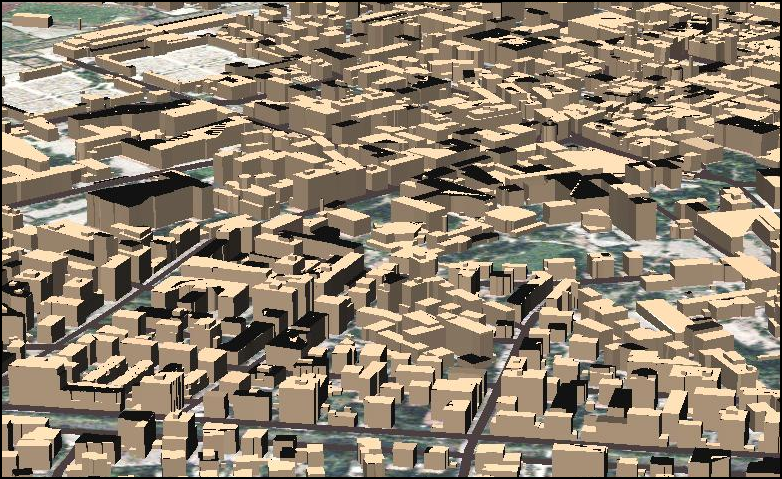
\includegraphics[width=0.75\mycolumnwidth]{Visualizacion_SIG/Extrusion.png}
\caption{\small La extrusi�n permite la creaci�n de objetos volum�tricos a partir de objetos planos. Los edificios de la imagen se han creado �nicamente a partir de la planta y un valor de altura para cada uno de ellos.}
\label{Fig:Extrusion} 
\end{figure}

	\item La dimensi�n vertical puede considerarse como otra variable visual alternativa. En relaci�n con lo comentado en el punto anterior, pueden crearse objetos volum�tricos mediante extrusi�n sin que la dimensi�n vertical de estos represente necesariamente una altura como tal, sino que est� en funci�n de un par�metro adicional. La figura \ref{Fig:Coropletas3D} muestra un ejemplo de esto. En la capa visualizada en la imagen, que representa la poblaci�n de una serie de estados, se ha empleado la elevaci�n para visualizar esta variable, adem�s de recurrir a la habitual gama de valores de colores. Se trata de un mapa de coropletas en el que, sin embargo, no se acude �nicamente a la variable visual color para simbolizar la componente tem�tica. En realidad, estamos utilizando esta junto a la variable tama�o, una variable que para el caso de pol�gonos no exist�a en la representaci�n bidimensional (existe, pero debe distorsionarse el contorno del pol�gono, algo que no resulta adecuado ya que este tiene un significado geogr�fico, o bien puede aplicarse sobre el grosor de la l�nea de contorno, lo cual no es tan f�cil de percibir e interpretar).

\begin{figure}[!hbt]
\centering
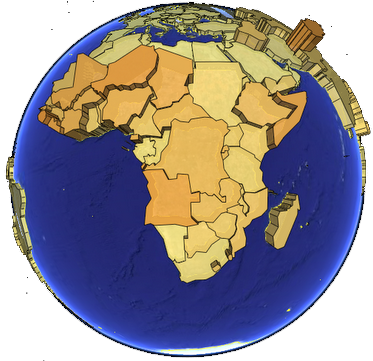
\includegraphics[width=0.55\mycolumnwidth]{Visualizacion_SIG/Coropletas3D.png}
\caption{\small La dimensi�n vertical puede emplearse como variable visual para visualizar la componente tem�tica de la informaci�n geogr�fica.}
\label{Fig:Coropletas3D} 
\end{figure}
	
	Un planteamiento similar se puede aplicar a capas r�ster, como se observa en la figura \ref{Fig:Superficie3D}. La superficie mostrada sobre el terreno no es un relieve procedente de una capa de elevaci�n, sino de una variable distinta (por ejemplo, presi�n o temperatura del aire), la cual, adem�s de simbolizarse mediante una rampa de colores, se representa en forma de relieve para hacer m�s evidente la variaci�n de esos valores. La capa no tiene componente vertical, ya que es una capa r�ster bidimensional, por lo que podemos utilizar esa tercera dimensi�n como variable visual. Hemos visto algunas visualizaciones as� en otras partes del libro, por ejemplo en la figura \ref{Fig:Coste_acumulado_3D}.
				
\begin{figure}
\centering
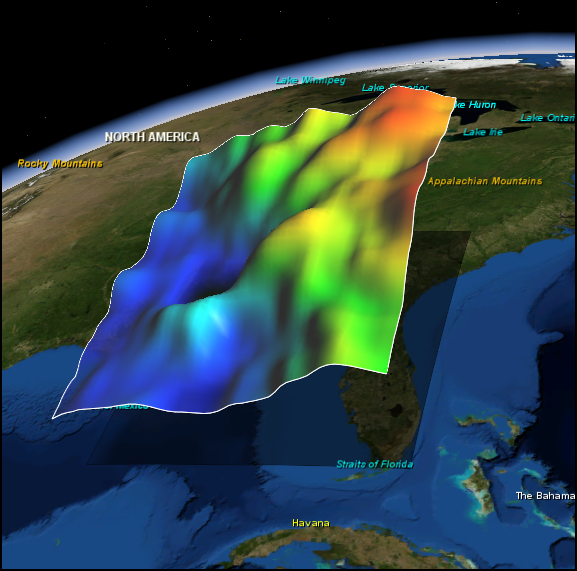
\includegraphics[width=0.5\mycolumnwidth]{Visualizacion_SIG/Superficie3D.png}
\caption{\small La dimensi�n vertical puede utilizarse tambi�n para simbolizar capas r�ster con variables distintas a la elevaci�n.}
\label{Fig:Superficie3D} 
\end{figure}

	\item Exageraci�n del relieve. Es habitual que en una visualizaci�n tridimensional exista alg�n modo de distorsionar el relieve para hacerlo m�s acusado. Mientras que las componentes $x$ e $y$ son proporcionales, la componente $z$ puede alterarse aplic�ndole un factor de escala para lograr que resulte m�s obvia la configuraci�n del relieve (Figura \ref{Fig:ExageracionRelieve}). Esto sirve para acentuar la morfolog�a del terreno, pero tambi�n puede ayudar a la comprensi�n de otras variables, especialmente si el relieve tiene influencia en ellas. Esta exageraci�n se aplica al propio relieve terrestre (es decir, al relieve de un terreno real), as� como al que puedan tener las distintas capas debido a la forma en que se representan, tal como en el ejemplo presentado en el punto anterior.\index{Exageraci�n del relieve}
	
\begin{figure}[!hbt]
\centering
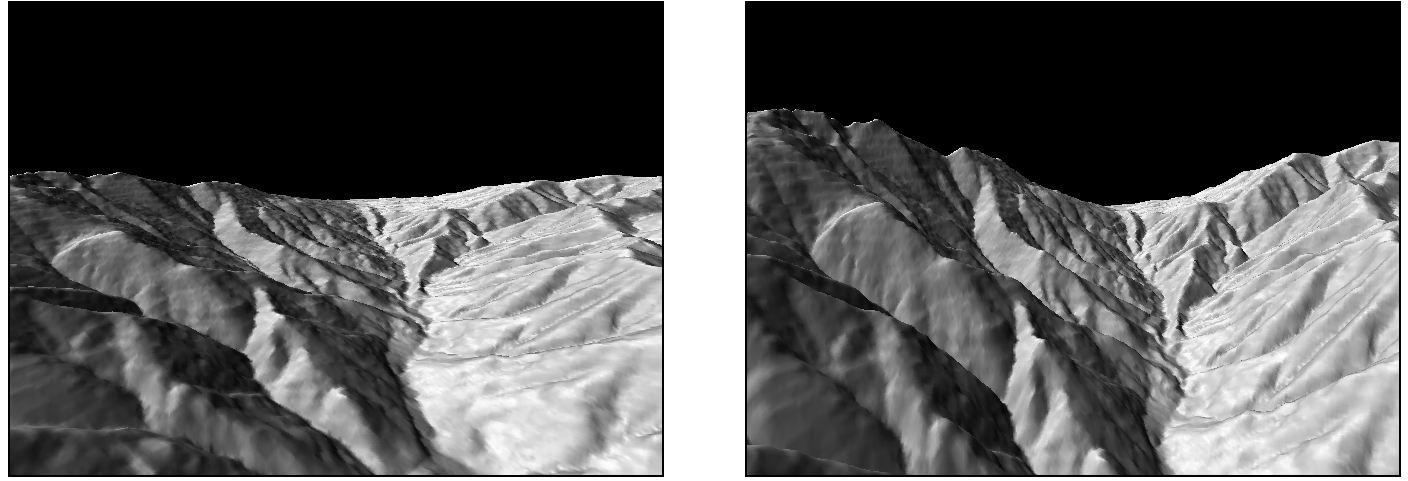
\includegraphics[width=0.95\mycolumnwidth]{Visualizacion_SIG/ExageracionRelieve.png}
\caption{\small La exageraci�n del relieve permite hacer m�s evidente la configuraci�n de este.}
\label{Fig:ExageracionRelieve} 
\end{figure}
	
\end{itemize}

Puede verse en lo anterior la necesidad de extender las ideas del dise�o cartogr�fico para considerar las peculiaridades de las vistas 3D, ya que si no se tienen estas en cuenta, los conceptos de la cartograf�a cl�sica, aunque imprescindibles igualmente en este caso, resultan no obstante insuficientes. M�s informaci�n sobre principios de dise�o cartogr�fico para vistas 3D puede encontrarse en \cite{HaeberlingDesign3D}.

\section{Visualizaci�n din�mica}

Mientras que un mapa impreso contiene una informaci�n est�tica que no var�a y que representa el estado de unas determinadas variables en un instante dado, dentro de un SIG podemos crear representaciones que vayan variando para mostrarnos la evoluci�n de esas variables. En un SIG es posible no solo visualizar una realidad, sino tambi�n el cambio que se produce en esa realidad. Esta visualizaci�n din�mica supone una herramienta de gran valor, especialmente para explorar la relaci�n entre distintas variables y c�mo el cambio de una de ellas afecta a las restantes.

La visualizaci�n din�mica se obtiene mediante una \emph{animaci�n}, la cual se compone de una serie de \emph{escenas}, del mismo modo que una pel�cula se compone de una serie de fotogramas. El mapa cl�sico representa una �nica de esas escenas, por lo que las nuevas posibilidades que una animaci�n aporta con respecto a este son notables. Aunque de manera distinta a la de una vista tridimensional, una animaci�n aporta tambi�n al mapa una dimensi�n adicional. 

El cambio que una animaci�n muestra no ha de darse necesariamente a lo largo del tiempo, sino que puede ser en el espacio o a medida que var�a cualquier otra variable. Por ejemplo, una animaci�n puede consistir en un trayecto a lo largo del cual se desplaza el observador y mostrar un <<vuelo>> entre dos puntos y c�mo var�a la realidad representada a medida que nos movemos. Este tipo de animaciones son muy comunes en los visores tridimensionales, que permiten definir el trayecto y los par�metros que establecen c�mo en los distintos puntos de este el observador mira al terreno.

Podemos, asimismo, escoger cualquier variable adicional como eje de la animaci�n. Imaginemos, por ejemplo, que disponemos de una capa con una serie de divisiones administrativas, y que para cada una de ellas conocemos el numero medio de hijos por pareja. Supongamos que esta informaci�n la tenemos adem�s divida por grupos en funci�n de sus ingresos medios anuales. Podemos crear tantos mapas de coropletas como clases haya establecidas en funci�n de esos ingresos, y simbolizar en cada una de ellas los pol�gonos correspondientes a las divisiones administrativas seg�n el n�mero de hijos. Si usamos esos mapas, cada uno de los cuales constituye una escena, para formar una animaci�n, esta mostrar� la variaci�n del n�mero de hijos en funci�n de los ingresos medios. Esa �ltima variable es el eje sobre el que se desplaza la animaci�n, y el tiempo y el espacio no han sido usados de modo alguno para crear esta.\index{Mapa!de coropletas}

Al la hora de crear una animaci�n, debemos tener en cuenta no solo las seis variables visuales que estudiamos en el cap�tulo \ref{Conceptos_basicos_visualizacion}, sino otras seis nuevas, las denominadas \emph{variables visuales din�micas}\cite{MacEachren1994Wiley}:

\index{Variables visuales!din�micas}

\begin{itemize}
	\item Momento. El equivalente a la variable visual posici�n, indica el momento en la animaci�n en que se produce un cambio de una escena a otra.
	\item Frecuencia. Indica la velocidad a la que se produce el cambio en la animaci�n. Si es demasiado lenta, puede aportar una longitud excesiva a esta, mientras que si es demasiado r�pida puede hacer dif�cil analizar e interpretar el cambio que se produce.
	\item Duraci�n. El tiempo que cada escena se encuentra visible, que no tiene que ser el mismo para todas ellas.
	\item Magnitud del cambio. Indica cu�nto cambia una escena respecto a la anterior. Si es peque�o, la animaci�n sera fluida, mientras que si es muy elevado, la animaci�n tendr� saltos bruscos. Dividido por la duraci�n nos indica la \emph{tasa de cambio}.
	\item Orden. La posici�n de cada escena dentro del conjunto, estableciendo antes o despu�s de cu�les de las restantes aparece.
	\item Sincronizaci�n. Si la animaci�n muestra la variaci�n de varias variables, establece c�mo el cambio en estas se encuentra relacionado. Una correcta sincronizaci�n ayuda a interpretar la relaci�n que puede existir entre las variables que var�an en la animaci�n.
\end{itemize}

En un entorno de visualizaci�n din�mica, el usuario pueden interactuar tambi�n con la representaci�n din�mica, alterando las caracter�sticas de la animaci�n del mismo modo que en una representaci�n est�tica dentro de un SIG puede modificar el encuadre haciendo uso de las herramientas de navegaci�n habituales.

\section{Otros elementos de visualizaci�n}

Adem�s de permitir una representaci�n distinta de los elementos cl�sicos del mapa y de las variables habituales, la visualizaci�n en un SIG puede ampliarse incorporando otros tipos de informaci�n distintos, que no tienen presencia en la cartograf�a tradicional. El ordenador es un soporte m�s potente que el mapa y soporta adem�s otros elementos no visuales, de tal modo que ofrece m�ltiples formas de enriquecer cualquier representaci�n.

En este sentido, el mapa puede comportarse no ya como un documento que trasmite un tipo particular de informaci�n (la de tipo geogr�fico), sino como un contenedor de muchas clases diferentes de informaci�n, todas ellas compartiendo el hecho de que pueden localizarse y posicionarse, y el mapa se convierte en el elemento de referencia desde el que acceder a todas ellas. Esta es una de las consecuencias del papel que los SIG han jugado haci�ndonos ver la importancia de la informaci�n espacial que la mayor�a de fen�menos tienen asociada, hasta el punto de que esa informaci�n geogr�fica, al ser puesta en un mapa, no constituye el objeto primordial de atenci�n, sino es una informaci�n com�n a otros muchos tipos de informaci�n, actuando como nexo de estos.

Algunos de los nuevos elementos que pueden a�adirse a una representaci�n en un SIG son los siguientes:


\begin{itemize}
	\item Fotograf�as. Aunque un mapa puede contener fotograf�as, est� muy limitado en temas de espacio, y la presencia de estas es anecd�tica. Por el contrario, y gracias a sus elementos interactivos, un SIG puede incorporar fotograf�as solo a una determinada escala, y solo si el usuario as� lo pide, haciendo clic por ejemplo en un s�mbolo concreto. Esto permite incorporar un n�mero ilimitado de im�genes, permitiendo que estas complementen a la informaci�n visual del propio mapa.
	
	Un caso particular son las fotograf�as de tipo inmersivo, en las que el usuario puede navegar a trav�s de fotograf�as del entorno como si se encontrara realmente en �l (Figura \ref{Fig:FotografiasInmersivas}).\index{Fotograf�as inmersivas}
	
\begin{figure}[!hbt]
\centering
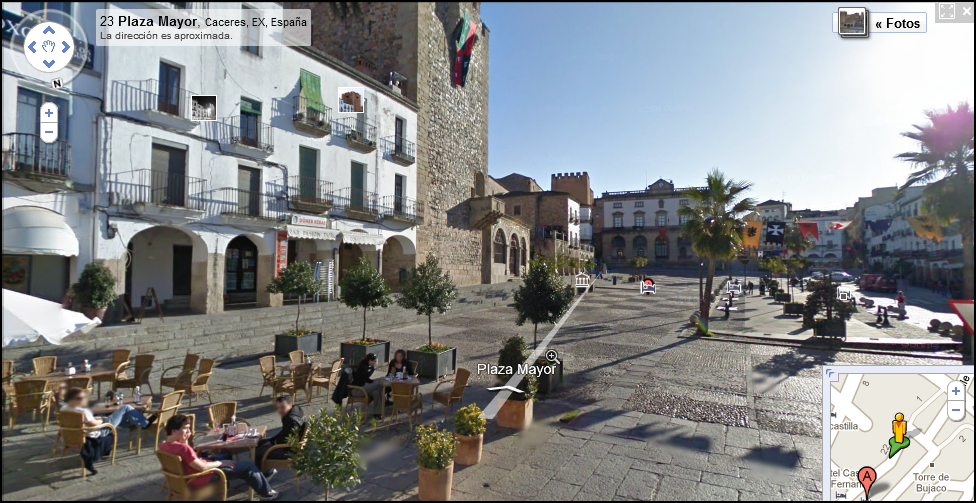
\includegraphics[width=0.85\mycolumnwidth]{Visualizacion_SIG/FotografiasInmersivas.png}
\caption{\small Las fotografias inmersivas permiten al usuario <<meterse>> en el mapa, ampliando la informaci�n que se muestra acerca de un lugar con im�genes reales tomadas sobre el terreno. Al igual que se navega por un mapa, el usuario puede navegar por el terreno haciendo uso de los controles interactivos correspondientes (imagen tomada de Google Street View).}
\label{Fig:FotografiasInmersivas} 
\end{figure}

	\item V�deos. Del mismo modo que las fotograf�as, aportan m�s informaci�n sobre la zona representada y permiten una exploraci�n mayor. Aunque son una tecnolog�a a�n muy experimental, existen tambi�n v�deos de tipo inmersivo.
	\item Sonido. Los elementos no han de ser necesariamente visuales, sino que pueden proporcionar informaci�n a trav�s de otros sentidos distintos.
	\item Documentos. Un SIG puede incorporar documentos complejos tales como p�ginas Web o textos varios.
\end{itemize}

Esta lista, no obstante, es muy susceptible de extenderse, ya que, virtualmente, un SIG puede incorporar cualquier elemento que pueda manejarse dentro de un ordenador. Cada d�a aparecen nuevas ideas sobre c�mo combinar la informaci�n geogr�fica con otros tipos de informaci�n, y el SIG se sit�a en la base de todos estos nuevos planteamientos como herramienta fundamental de trabajo.

\section{Resumen}

Hemos visto en este cap�tulo c�mo aplicar las ideas de cap�tulos previos a la representaci�n de capas en un SIG. Cada tipo de capa tiene sus particularidades, y es en funci�n de estas como hemos analizado la mejor forma de emplear las variables visuales y los conceptos de simbolog�a gr�fica que ya conocemos para simbolizar la informaci�n geogr�fica e incorporarla a un mapa.

Puesto que una parte de las representaciones que generamos en un SIG est�n destinadas a ser representadas en pantalla, hemos analizado igualmente las implicaciones que esto tiene a la hora de crear visualizaciones a partir de la informaci�n geogr�fica con la que trabajamos. Dos son los principales aspectos que han de tenerse en cuenta: la baja resoluci�n de la pantalla en comparaci�n con el papel y la interactividad propia de la representaci�n.

Adem�s de trabajar con las formas cartogr�ficas cl�sicas que un SIG es capaz de producir, existen nuevas formas que tambi�n hemos detallado, entre las que destacan las vistas tridimensionales y las animaciones. Junto a ellas, una de las tendencias actuales que aumentan las posibilidades de un SIG como herramienta de visualizaci�n es la incorporaci�n de otros elementos tales como v�deos, fotograf�as u otros documentos de diversas clases. 


